\documentclass[a4paper, 12pt]{report}

\usepackage[dvipsnames]{xcolor}

%%%%%%%%%%%%%%%%
% Set Variables %
%%%%%%%%%%%%%%%%

\def\useItalian{0}  % 1 = Italian, 0 = English

\def\courseName{Advanced Algorithms}

\def\coursePrerequisites{\begin{itemize} \item Progettazione degli Algoritmi \end{itemize}}

% \def\book{TODO}

% \def\authorName{Simone Bianco}
% \def\email{bianco.simone@outlook.it}
% \def\github{https://github.com/Exyss/university-notes}
% \def\linkedin{https://www.linkedin.com/in/simone-bianco}

\def\authorName{Alessio Bandiera}
\def\email{alessio.bandiera02@gmail.com}
\def\github{https://github.com/aflaag-notes}
\def\linkedin{https://www.linkedin.com/in/alessio-bandiera-a53767223}

%%%%%%%%%%%%
% Packages %
%%%%%%%%%%%%

\usepackage{../../packages/Nyx/nyx-packages}
\usepackage{../../packages/Nyx/nyx-styles}
\usepackage{../../packages/Nyx/nyx-frames}
\usepackage{../../packages/Nyx/nyx-macros}
\usepackage{../../packages/Nyx/nyx-title}
\usepackage{../../packages/Nyx/nyx-intro}

%%%%%%%%%%%%%%
% Title-page %
%%%%%%%%%%%%%%

\logo{../../packages/Nyx/logo.png}

\if\useItalian1
    \institute{\curlyquotes{\hspace{0.25mm}Sapienza} Università di Roma}
    \faculty{Ingegneria dell'Informazione,\\Informatica e Statistica}
    \department{Dipartimento di Informatica}
    \ifdefined\book
        \subtitle{Appunti integrati con il libro \book}
    \fi
    \author{\textit{Autore}\\\authorName}
\else
    \institute{\curlyquotes{\hspace{0.25mm}Sapienza} University of Rome}
    \faculty{Faculty of Information Engineering,\\Informatics and Statistics}
    \department{Department of Computer Science}
    \ifdefined\book
        \subtitle{Lecture notes integrated with the book \book}
    \fi
    \author{\textit{Author}\\\authorName}
\fi


\title{\courseName}
\date{\today}

% \supervisor{Linus \textsc{Torvalds}}
% \context{Well, I was bored\ldots}

\addbibresource{./references.bib}

%%%%%%%%%%%%
% Document %
%%%%%%%%%%%%

\begin{document}
    \maketitle

    % The following style changes are valid only inside this scope 
    {
        \hypersetup{allcolors=black}
        \fancypagestyle{plain}{%
        \fancyhead{}        % clear all header fields
        \fancyfoot{}        % clear all header fields
        \fancyfoot[C]{\thepage}
        \renewcommand{\headrulewidth}{0pt}
        \renewcommand{\footrulewidth}{0pt}}

        \romantableofcontents
    }

    \introduction

    %%%%%%%%%%%%%%%%%%%%%

    \chapter{Approximation algorithms}

    TODO \todo{missing introduction}

    Lastly, \underline{\tit{unless specified}} we will adopt the following convention in these notes, when talking about \tbf{approximation algorithm}. Given a problem P for which there is an optimal solution OPT, and an algorithm that solves P which outputs a solution ALG to P

    \begin{itemize}
        \item if P is a \tbf{minimization} problem, we say that $A$ yields an $\alpha$-approximation of P if $$\mathrm{ALG} \le \alpha \cdot \mathrm{OPT}$$ in which $\alpha \in \R_{> 1}$
        \item if $P$ is a \tbf{maximization} problem, we say that $A$ yields an $\alpha$-approximation of P if $$\mathrm{ALG} \ge \alpha \cdot \mathrm{OPT}$$ in which $\alpha \in (0, 1]$
    \end{itemize}

    \section{Approximation through randomness}

    \subsection{The Maximum Cut problem} \label{maxcut}

    The first problem that will be discussed is the \href{https://en.wikipedia.org/wiki/Maximum_cut}{Maximum Cut} problem. The \tbf{Maximum Cut problem} --- in the unweighted case --- is a classic combinatorial optimization problem in the branch of \href{https://en.wikipedia.org/wiki/Graph_theory}{graph theory}, in which we seek to partition the vertices of an undirected graph into two disjoint subsets, while maximizing the number of edges that have endpoints in both subsets. More formally, we will define a \tbf{cut} of a graph as follows.

    \begin{frameddefn}{Cut}
        Given an undirected graph $G = (V, E)$, and two disjoint subsets $S, T \subseteq V$, the \tbf{cut} induced by $S$ and $T$ on $G$ is defined as follows $$\mathrm{cut}(S, T) = \{e \in E : \abs{S \cap e} = \abs{T \cap e} = 1\}$$ In the case in which $T = \overline S = V - S$ we will simply write $\mathrm{cut}(S) = \mathrm{cut}(S, \overline S)$.
    \end{frameddefn}

    Note that in the definition above we are defining the cut of a graph through the intersection between a set of vertices and edges in $E$; this is because, in the undirected case, we will consider the edges of a graph $G = (V, E)$ as sets of 2 elements $$E = \{\{u, v\} \mid u, v \in V\}$$ Therefore, given two sets of vertices $S$ and $T$, the cut induced by $S$ and $T$ is simply the set of edges that have only one endpoint in $S$ and the other one in $T$.

    \begin{figure}[H]
        \centering
        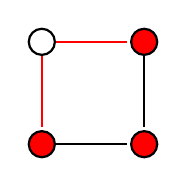
\begin{tikzpicture}[-,>=stealth,shorten >=1pt,auto,node distance=1.3cm, thick,main node/.style={scale=0.9,circle,draw,font=\sffamily\normalsize}]

            \node[circle, draw]  (1) []{};
            \node[circle, draw, fill=red]  (2) [below of = 1]{};
            \node[circle, draw, fill=red]  (3) [right of = 1]{};
            \node[circle, draw, fill=red]  (4) [below of = 3]{};

            % \path[every node/.style={font=\sffamily\small}]

            \draw[-] (1) [red] to (2);
            \draw[-] (1) [red] to (3);
            \draw[-] (2) to (4);
            \draw[-] (3) to (4);

            ;
        \end{tikzpicture}
        \caption{Given the set of red vertices $S$, the green edges represent $\mathrm{cut}(S)$.}
    \end{figure}

    With this definition, we can introduce the \tbf{Maximum Cut} problem, which is defined as follows.

    \begin{frameddefn}{Maximum Cut problem}
        The \tbf{Maximum Cut} (MC) problem is defined as follows: given an undirected graph $G = (V, E)$, determine the set $S \subseteq V$ that maximizes $\abs{\mathrm{cut}(S)}$.
    \end{frameddefn}

    Although this problem is known to be \textsf{APX}-hard \cite{maxcut}, approximation algorithms and heuristic methods like \tit{greedy algorithms} and \tit{local search} are commonly used to find near-optimal solutions.

    For now, we present the following \tbf{randomized algorithm}, which provides a straightforward $\frac{1}{2}$-approximation for MC. This algorithm runs in polynomial time and achieves the approximation guarantee with high probability.

    \begin{framedalgo}[label={max cut alg}]{Random Cut}
        Given an undirected graph $G = (V, E)$, the algorithm returns a cut of $G$. \\
        \hrule

        \quad
        \begin{algorithmic}[1]
            \Function{RandomCut}{$G$}
                \State $S := \varnothing$
                \For{$v \in V$}
                    \State Let $c_v$ be the outcome of the flip of an independent fair coin
                    \If{$c_v == \mathrm H$}
                        \State $S = S \cup \{v\}$
                    \EndIf
                \EndFor
                \State \textbf{return} $S$
            \EndFunction
        \end{algorithmic}
    \end{framedalgo}

    Note that this algorithm is powerful, because \tit{it does not care about the structure of the graph in input}, since the output is completely determined by the coin flips performed in the \texttt{for} loop. Now we will prove that this algorithm provides a correct \tbf{expected $\frac{1}{2}$-approximation} of MC.
    
    \begin{framedthm}[label={expected random cut}]{}
        Let $G= (V, E)$ be a graph, and let $S^*$ be an optimal solution to MC on $G$. Then, given $S = \textsc{RandomCut}(G)$, it holds that $$\mathbb E [\abs{\mathrm{cut}(S)}] \ge \dfrac{1}{2} \abs{\mathrm{cut}(S^*)}$$
    \end{framedthm}

    \begin{proof}
        By definition, note that $$\forall e \in E \quad e \in \mathrm{cut}(S) \iff \abs{S \cap e} = 1$$ Consider an edge $e = \{v, w\} \in E$; then, by definition $$\{v, w\} \in \mathrm{cut}(S) \iff (v \in S \land w \notin S) \lor (v \notin S \land w \in S)$$ and let $\xi_1$ and $\xi_2$ be these last two events respectively. Then $$\Pr[\xi_1] = \Pr[c_v = \mathrm{heads} \land c_w = \mathrm{tails}]$$ by definition of the algorithm, and by independence of the flips of the fair coins we have that $$\Pr[\xi_1] = \Pr[c_v = \mathrm{heads}] \cdot \Pr[c_w = \mathrm{tails}] = \dfrac{1}{2} \cdot \dfrac{1}{2} = \dfrac{1}{4}$$ Analogously, we can show that $$\Pr[\xi_2] = \dfrac{1}{4}$$ This implies that $$\Pr[e \in \mathrm{cut}(S)] = \Pr[\xi_1 \lor \xi_2] = \Pr[\xi_1] + \Pr[\xi_2] - \Pr[\xi_1 \land \xi_2] = \dfrac{1}{4} + \dfrac{1}{4} - 0 = \dfrac{1}{2}$$ Hence, we have that $$\mathbb E [\abs{\mathrm{cut}(S)}] = \sum_{e \in E}{1 \cdot \Pr[e \in \mathrm{cut}(S)]} = \dfrac{\abs E}{2} \ge \dfrac{\abs{\mathrm{cut}(S^*)}}{2}$$ where the last inequality directly follows from the definition of cut of a graph.
    \end{proof}

    As previously mentioned, this algorithm has an \tbf{expected approximation ratio} of $\frac{1}{2}$, which implies that it may return very bad solutions in some cases, depending on the outcomes of the coin flips. However, thanks to the following algorithm, we can actually transform the \tbf{guarantee of expectations} into a \tbf{guarantee of high probability} --- note that it is possible to show that the previous algorithm provides guarantee of high probability as well, but the proof is much more complex.

    \begin{framedalgo}{$t$-times Random Cut}
        Given an undirected graph $G = (V, E)$ and an integer $t > 0$, the algorithm returns a cut of $G$. \\
        \hrule

        \quad
        \begin{algorithmic}[1]
            \Function{$t$-timesRandomCut}{$G$, $t$}
                \For{$i \in [t]$}
                    \State $S_i := \textsc{RandomCut}(G)$
                \EndFor
                \State \textbf{return} $S \in \argmax_{i \in [t]}{\abs{\mathrm{cut}(S_i)}}$
            \EndFunction
        \end{algorithmic}
    \end{framedalgo}

    The algorithm above simply runs the \textsc{RandomCut} algorithm $t$ times, and returns the set $S_i$ that maximizes the cut, among all the various $S_1, \ldots, S_t$. The following theorem will show that a \tit{reasonable number} of runs of the \textsc{RandomCut} algorithm suffices in order to almost certainly obtain a $\approx \frac{1}{2}$-approximation of any optimal solution.

    \begin{framedthm}{}
        Let $G= (V, E)$ be a graph, and let $S^*$ be an optimal solution to MC on $G$. Then, given $S = \textsc{$t$-timesRandomCut}(G, t)$, it holds that $$\Pr \sbk{\abs{\mathrm{cut}(S)} > \dfrac{1 - \varepsilon}{2} \abs{\mathrm{cut}(S^*)}} > 1 - \delta$$ where $t = \frac{2}{\varepsilon} \ln {\frac{1}{\delta}}$ and $0 < \varepsilon, \delta < 1$.
    \end{framedthm}
    
    \begin{proof}
        For each $i \in [t]$, let $C_i := \abs{\mathrm{cut}(S_i)}$ for each $S_i$ defined by the algorithm, and let $N_i := \abs E - C_i$. Let $0 < \varepsilon < 1$; since $N_i$ is a non-negative random variable, by \href{https://en.wikipedia.org/wiki/Markov%27s_inequality}{Markov's inequality} we have that $$\Pr[N_i \ge (1 + \varepsilon) \mathbb E [N_i]] \le \dfrac{1}{1 + \varepsilon} = 1 - \dfrac{\varepsilon}{1 + \varepsilon} \le 1 - \dfrac{\varepsilon}{2}$$ In particular, this inequality can be rewritten as follows:
        \begin{equation*}
            \begin{split}
                1 - \dfrac{\varepsilon}{2} &\ge \Pr[N_i \ge (1 + \varepsilon) \mathbb E [N_i]] \\
                                           &= \Pr[\abs E - C_i \ge (1 + \varepsilon)(\abs E - \mathbb E [C_i])] \\
                                           &= \Pr[- \varepsilon \abs E \ge C_i - (1 + \varepsilon) \mathbb E [C_i]]
            \end{split}
        \end{equation*}
        As shown in the proof of \cref{expected random cut}, we know that $\mathbb E [C_i] = \frac{\abs E}{2}$, therefore
        \begin{equation*}
            \begin{split}
                1 - \dfrac{\varepsilon}{2} &\ge \Pr[- \varepsilon \abs E \ge C_i - (1 + \varepsilon) \mathbb E [C_i]] \\
                                           &= \Pr \sbk{- \varepsilon \abs E \ge C_i - \dfrac{1 + \varepsilon}{2} \abs E} \\
                                           &= \Pr \sbk{- \varepsilon \dfrac{\abs E}{2} \ge C_i - \dfrac{\abs E}{2}} \\
                                           &= \Pr \sbk{\dfrac{1 - \varepsilon}{2} \abs E\ge C_i} \\
                                           &= \Pr \sbk{(1 - \varepsilon) \mathbb E[C_i] \ge C_i} \\
            \end{split}
        \end{equation*}
        Note that the event in the last probability, namely $$\abs{\mathrm{cut}(S_i)}  \le (1 - \varepsilon) \mathbb E [\abs{\mathrm{cut}(S_i)}]$$ corresponds to a \curlyquotes{bad} solution, i.e. one whose cardinality is at most $(1 - \varepsilon)$-th of the expected value.

        By definition of the algorithm, each of the $t$ runs of the \textsc{RandomCut} algorithm is independent from the others, therefore the probability of \tit{all} the solutions $S_1, \ldots, S_t$ being \curlyquotes{bad} is bounded by $$\Pr[\forall i \in [t]  \quad C_i \le (1 - \varepsilon) \mathbb E [C_i]] = \prod_{i = 1}^t{\Pr[C_i \le (1 - \varepsilon)\mathbb E[C_i]]} \le \rbk{1 - \dfrac{\varepsilon}{2}}^t$$

        Using the fact that $$\forall x \in \R \quad 1 - x \le e^{-x} \implies 1 - \frac{\varepsilon}{2} \le e^{- \frac{\varepsilon}{2}}$$ we have that $$\Pr[\forall i \in [t] \quad C_i \le (1 - \varepsilon) \mathbb E[C_i]] \le \rbk{1 - \dfrac{\varepsilon}{2}}^t \le e^{- \frac{\varepsilon}{2} \cdot t} = e^{- \ln {\frac{1}{\delta}}} = \delta$$

        Therefore, the probability that at least one among $S_1, \ldots, S_t$ is a \curlyquotes{good} solution is bounded by $$\Pr[\exists i \in [t] \quad C_i > (1 - \varepsilon) \mathbb E [C_i]] = 1 - \Pr[\forall i \in [t] \quad C_i \le (1 - \varepsilon) \mathbb E [C_i]] \ge 1 - \delta$$

        Finally, since the $\argmax$ operation in the algorithm will select in the \curlyquotes{worst} case such good solution, we conclude that
        \begin{equation*}
            \begin{split}
                \Pr \sbk{\abs{\mathrm{cut}(S)} > \dfrac{1 - \varepsilon}{2} \abs{\mathrm{cut}(S^*)}} &\ge \Pr \sbk {\exists i \in [t] \quad C_i > \dfrac{1 - \varepsilon}{2} \abs{\mathrm{cut}(S^*)}} \\
                                                                                                     &\ge \Pr[\exists i \in [t] \quad C_i > (1 - \varepsilon) \Exp[C_i]] \\
                                                                                                     &\ge 1 - \delta
            \end{split}
        \end{equation*}
    \end{proof}

    Note that this result is \tit{very powerful}: for instance, if $\varepsilon = \delta = 0.1$, we get that $$\Pr[\abs{\mathrm{cut}(S)} > 0.45 \cdot \abs{\mathrm{cut}(S^*)}] \ge 0.9$$ and $t \approx 46$, meaning that we just need to run the \textsc{RandomCut} algorithm approximately 46 times in order to get a solution that is better than a $0.45$-approximation with $90\%$ probability.

    In later sections we will present a 0.878-approximation of MC, based on a \tit{very} different approach.

    \section{Approximation through reduction}

    \subsection{The Vertex Cover problem}

    Another very important problem in graph theory is the \href{https://en.wikipedia.org/wiki/Vertex_cover}{Vertex Cover} problem, which concerns the combinatorial structure of the \tbf{vertex cover}, defined as follows.

    \begin{frameddefn}{Vertex cover}
        Given an undirected graph $G = (V, E)$, a \tbf{vertex cover} of $G$ is a set of vertices $S \subseteq V$ such that $$\forall e \in E \quad \exists v \in S \quad v \in e$$
    \end{frameddefn}

    \begin{figure}[H]
        \centering
        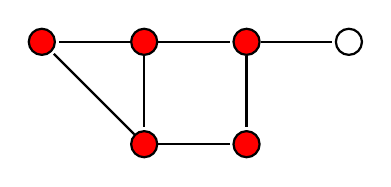
\begin{tikzpicture}[-,>=stealth,shorten >=1pt,auto,node distance=1.3cm, thick,main node/.style={scale=0.9,circle,draw,font=\sffamily\normalsize}]

            \node[circle, draw, fill=red] (1) []{};
            \node[circle, draw, fill=red] (2) [right of = 1]{};
            \node[circle, draw, fill=red] (3) [below of = 1]{};
            \node[circle, draw, fill=red] (4) [below of = 2]{};
            \node[circle, draw, fill=red] (5) [left of = 1]{};
            \node[circle, draw, ] (6) [right of = 2]{};

            \draw[-] (1) to (2);
            \draw[-] (1) to (3);
            \draw[-] (2) to (4);
            \draw[-] (1) to (5);
            \draw[-] (3) to (4);
            \draw[-] (3) to (5);
            \draw[-] (2) to (6);

            ;
        \end{tikzpicture}
        \caption{An example of a vertex cover.}
    \end{figure}

    As shown in figure, a vertex cover is simply a set of vertices that must \tit{cover} all the edges of the graph. Clearly, the trivial vertex cover is representd by $S = V$, but a more interesting solution to the problem is represented by the \tbf{minimum vertex cover}.

    \begin{frameddefn}{Vertex Cover problem}
        The \tbf{Vertex Cover} (VC) problem is defined as follows: given an undirected graph $G = (V, E)$, determine the vertex cover $S \subseteq V$ of smallest cardinality.
    \end{frameddefn}

    \begin{figure}[H]
        \centering
        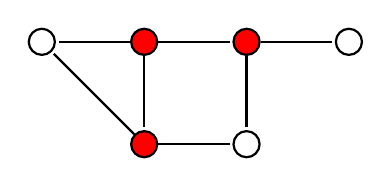
\begin{tikzpicture}[-,>=stealth,shorten >=1pt,auto,node distance=1.3cm, thick,main node/.style={scale=0.9,circle,draw,font=\sffamily\normalsize}]

            \node[circle, draw, fill=red] (1) []{};
            \node[circle, draw, fill=red] (2) [right of = 1]{};
            \node[circle, draw, fill=red] (3) [below of = 1]{};
            \node[circle, draw, ] (4) [below of = 2]{};
            \node[circle, draw, ] (5) [left of = 1]{};
            \node[circle, draw, ] (6) [right of = 2]{};

            \draw[-] (1) to (2);
            \draw[-] (1) to (3);
            \draw[-] (2) to (4);
            \draw[-] (1) to (5);
            \draw[-] (3) to (4);
            \draw[-] (3) to (5);
            \draw[-] (2) to (6);

            ;
        \end{tikzpicture}
        \caption{This is the \tit{minimum vertex cover} of the previous graph.}
    \end{figure}

    As famously proved by \textcite{karp} in 1972, this problem is \NPclass-complete, hence we are interested in finding algorithms that allow to find approximations of optimal solutions. For instance, an algorithm that is able to approximate VC concerns the \href{https://en.wikipedia.org/wiki/Matching_(graph_theory)}{matching} problem.

    \begin{frameddefn}{Matching}
        Given an undirected graph $G = (V, E)$, a \tbf{matching} of $G$ is a set of edges $A \subseteq E$ such that $$\forall e, e' \in A \quad e \cap e' = \varnothing$$
    \end{frameddefn}

    \begin{figure}[H]
        \centering
        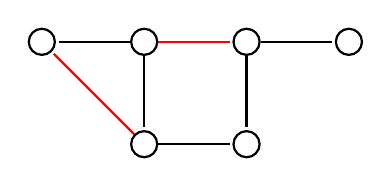
\begin{tikzpicture}[-,>=stealth,shorten >=1pt,auto,node distance=1.3cm, thick,main node/.style={scale=0.9,circle,draw,font=\sffamily\normalsize}]

            \node[circle, draw] (1) []{};
            \node[circle, draw] (2) [right of = 1]{};
            \node[circle, draw] (3) [below of = 1]{};
            \node[circle, draw] (4) [below of = 2]{};
            \node[circle, draw] (5) [left of = 1]{};
            \node[circle, draw] (6) [right of = 2]{};

            \draw[-] (1) [red] to (2);
            \draw[-] (1) to (3);
            \draw[-] (2) to (4);
            \draw[-] (1) to (5);
            \draw[-] (3) to (4);
            \draw[-] (3) [red] to (5);
            \draw[-] (2) to (6);

            ;
        \end{tikzpicture}
        \caption{A \tit{matching} of the previous graph.}
        \label{matching}
    \end{figure}

    As shown in figure, a matching is nothing more than a set of edges that must not share endpoints with each other --- for this reason, in literature it is often referred to as \tbf{independent edge set}. Differently from the vertex cover structure, in this context the trivial matching is clearly the set $A = \varnothing$, which vacuously satisfies the matching condition. However, a more interesting solution is represented by the \tbf{maximum matching}, but this time we have to distinguish two slightly different definitions, namely the concept of \tit{maximal} and \tit{maximum}.

    \begin{frameddefn}{Maximal matching}
        A \tbf{maximal matching} is a matching that cannot be extended any further.
    \end{frameddefn}
    
    For instance, the matching shown in \cref{matching} is actually a \tbf{maximal matching}, because no other edge in $E$ can be added to the current set of edges $A$ of the matching without breaking the matching condition.

    \begin{frameddefn}{Maximum matching}
        A \tbf{maximum matching} is a matching that has the largest cardinality.
    \end{frameddefn}
    
    Clearly, the previous example does not represent a \tbf{maximum matching}, because the following set of edges

    \begin{figure}[H]
        \centering
        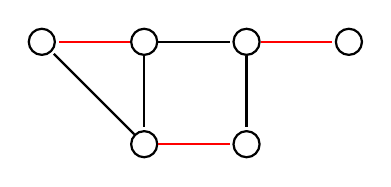
\begin{tikzpicture}[-,>=stealth,shorten >=1pt,auto,node distance=1.3cm, thick,main node/.style={scale=0.9,circle,draw,font=\sffamily\normalsize}]

            \node[circle, draw] (1) []{};
            \node[circle, draw] (2) [right of = 1]{};
            \node[circle, draw] (3) [below of = 1]{};
            \node[circle, draw] (4) [below of = 2]{};
            \node[circle, draw] (5) [left of = 1]{};
            \node[circle, draw] (6) [right of = 2]{};

            \draw[-] (1) to (2);
            \draw[-] (1) to (3);
            \draw[-] (2) to (4);
            \draw[-] (1) [red] to (5);
            \draw[-] (3) [red] to (4);
            \draw[-] (3) to (5);
            \draw[-] (2) [red] to (6);

            ;
        \end{tikzpicture}
    \end{figure}

    is still a valid matching for the graph, but has a larger cardinality than the previous set.

    Differently from VC, a \tit{maximum matching} can be found in polynomial time. Moreover, the following algorithm can be used to determine a \tit{maximal matching} of a given graph.

    \begin{framedalgo}{Maximal matching}
        Given an undirected graph $G = (V, E)$, the algorithm returns a maximal matching of $G$. \\
        \hrule

        \quad
        \begin{algorithmic}[1]
            \Function{MaximalMatching}{$G$}
                \State $S := \varnothing$
                \While{$E \neq \varnothing$}
                    \State Choose $e\in E$
                    \State $S = S \cup \{e\}$
                    \State Remove from $E$ all the edges incident on $u$ or on $v$
                    \State $E = E - \{e\}$
                \EndWhile
                \State \textbf{return} $S$
            \EndFunction
        \end{algorithmic}
    \end{framedalgo}

    \idea{
        The algorithm is very straightforward: at each iteration, a random edge $e = \{u, v\}$ is chosen from $E$, and then any edge $e' \in E$ such that $e \cap e' \neq \varnothing$ is removed from $E$.

        Clearly, line 6 ensures that the output is a \tit{matching}, and the terminating condition of the \texttt{while} loop ensures that it is \tit{maximal}, but since the output depends on the chosen edges, $S$ is not guaranteed to be \tit{maximum}.
    }

    Another major reason on why we focus on matchings is the following theorem.

    \begin{framedthm}{Matchings bound vertex covers}
        Given an undirected graph $G = (V, E)$, a matching $A \subseteq E$ of $G$, and a vertex cover $S \subseteq V$ of $G$, we have that $\abs S \ge \abs A$.
    \end{framedthm}

    \begin{proof}
        By definition, any vertex cover $S$ of $G = (V, E)$ is also a vertex cover for $G^B = (V, B)$, for any set of edges $B \subseteq E$, and in particular this is true for $G^A = (V, A)$.

        Now consider $G^A$, and a vertex cover $C$ on it: by construction we have that $\Delta \le 1$, therefore any vertex in $C$ will cover at most 1 edge of $A$. This implies that if $\abs C = k$, then $C$ will cover at most $k$ edges of $G^A$.

        Lastly, since $G^A$ has $\abs A$ edges by definition, any vertex cover defined on $G^A$ has to contain at least $\abs A$ vertices. This implies that no vertex cover $S$ of $G$ smaller than $\abs A$ can exist, because $S$ will have to cover at least the edges in $A$.
    \end{proof}
    
    Thanks to this theorem, we can easily show that the algorithm that we just presented in order to find maximal matchings is a 2-approximation of VC. 

    \begin{framedthm}{}
        Given a graph $G$, and $M = \textsc{MaximalMatching}(G)$, let $S := \bigcup_{e \in M}{e}$. Then $S$ is a 2-approximation of VC on $G$.
    \end{framedthm}

    \begin{proof}
        Consider an optimal solution $S^*$ to VC on $G$, and let $M = \{e_1, \ldots, e_t\}$. Note that at each iteration of the algorithm exactly 1 edge is added to $M \subseteq V$, hence it always holds that $$S_i \cap S_{i + 1} = e_i = \{u, v\}$$ for any iteration $i \in [t - 1]$. Moreover, since $M$ is a matching, it holds that $\forall e, e' \in M \quad e \cap e' = \varnothing$, therefore $\abs{S} = 2 \abs{M}$. Finally, by the previous theorem we have that $\abs{M} \le \abs{S^*}$, concluding that $$\abs S = 2 \abs M \le 2 \abs{S^*}$$
    \end{proof}
    
    This 2-approximation algorithm is conjectured to be optimal, but it has not been proven yet. In fact, VC is conjectured to be \NPclass-hard to $(2 - \varepsilon)$-approximate, for any $\varepsilon > 0$.

    Interestingly, the decisional version of VC is \href{https://en.wikipedia.org/wiki/Parameterized_complexity#FPT}{Fixed Parameter Tractable}. This characterization comes from the nature of the problem: for each edge $e = \{u, v\}$ of a given undirected graph $G = (V, E)$, either $u$ or $v$ has to be in the vertex cover, therefore it possible to approach VC by trying all possible choices of set of vertices $S \subseteq V$, and backtrack if necessary. The following algorithm employs this idea.

    \begin{framedalgo}{Decisional VC}
        Given an undirected graph $G = (V, E)$, and an integer $k$, the algorithm returns \texttt{True} if and only if $G$ admits a vertex cover of size $k$. \\
        \hrule

        \quad
        \begin{algorithmic}[1]
            \Function{VC}{$G$, $k$}
                \If{$E == \varnothing$}
                    \State \tbf{return} \texttt{True}
                \ElsIf{$k == 0$}
                    \State \tbf{return} \texttt{False}
                \Else
                    \State Choose $e = \{u, v\} \in E$
                    \If{$\textsc{VC}(G[V - \{u\}]), k - 1)$}
                        \State \tbf{return} \texttt{True}
                    \EndIf
                    \If{$\textsc{VC}(G[V - \{v\}]), k - 1)$}
                        \State \tbf{return} \texttt{True}
                    \EndIf
                    \State \tbf{return} \texttt{False}
                \EndIf
            \EndFunction
        \end{algorithmic}
    \end{framedalgo}

    Note that this algorithm actually solves the \tit{decisional} version of VC. Moreover, the algorithm uses the definition of \tbf{induced subgraph}, which is the following.

    \begin{frameddefn}{Induced subgraph}
        Given a graph $G = (V, E)$, and a set of vertices $S \subseteq V$, then $G[S]$ represents the \tbf{subgraph induced by $S$ on $G$}, obtained by removing from $G$ all the nodes of $V - S$ and the edges incident on them.
    \end{frameddefn}

     \begin{figure}[H]
        \centering

        \begin{tabular}{ccc}
            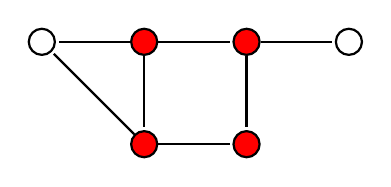
\begin{tikzpicture}[-,>=stealth,shorten >=1pt,auto,node distance=1.3cm, thick,main node/.style={scale=0.9,circle,draw,font=\sffamily\normalsize}]

                \node[circle, draw, fill=red] (1) []{};
                \node[circle, draw, fill=red] (2) [right of = 1]{};
                \node[circle, draw, fill=red] (3) [below of = 1]{};
                \node[circle, draw, fill=red] (4) [below of = 2]{};
                \node[circle, draw] (5) [left of = 1]{};
                \node[circle, draw] (6) [right of = 2]{};

                \draw[-] (1) to (2);
                \draw[-] (1) to (3);
                \draw[-] (2) to (4);
                \draw[-] (1) to (5);
                \draw[-] (3) to (4);
                \draw[-] (3) to (5);
                \draw[-] (2) to (6);

                ;
            \end{tikzpicture}

            &\qquad\qquad&

            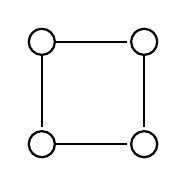
\begin{tikzpicture}[-,>=stealth,shorten >=1pt,auto,node distance=1.3cm, thick,main node/.style={scale=0.9,circle,draw,font=\sffamily\normalsize}]

                \node[circle, draw] (1) []{};
                \node[circle, draw] (2) [right of = 1]{};
                \node[circle, draw] (3) [below of = 1]{};
                \node[circle, draw] (4) [below of = 2]{};

                \draw[-] (1) to (2);
                \draw[-] (1) to (3);
                \draw[-] (2) to (4);
                \draw[-] (3) to (4);

                ;
            \end{tikzpicture}
        \end{tabular}

        \caption{On the left: a graph $G$ and a set of vertices $S$. On the right: the graph $G[S]$.}
    \end{figure}

    \idea{
        The structure of the algorithm consists of a simple backtracking algorithm:
        \begin{itemize}
            \item if the current graph has no edges, we covered every edge of the graph, therefore we return \texttt{True}
            \item if the current graph has some edges, but $k = 0$, then $G$ does not admit a vertex cover of size $k$, thus we return \texttt{False}
            \item if the current graph has some edges, and $k \neq 0$, then we choose an edge $e = \{u, v\} \in E$ arbitrarily, and we try to consider first $u$ then $v$ in a possible vertex cover --- note that $G[V - \{x\}]$ is a graph that does not contain $x$, neither any edge adjacent to it; if both attempts fail, we return \texttt{False}
        \end{itemize}
    }

    \cost{
        It is easy to see that the cost directly depends on the number of recursive calls that the algorithm performs, which is $2^k$ in the worst case, and the cost of constructing $G[V - \{x\}]$, which we can assume to be $O\rbk{n^2}$. Hence, the algorithm has a total cost of $O \rbk{2^k \cdot n^2}$.
    }

    \chapter{Mathematical Programming}

    Up to this point, we have introduced several \NPclass-complete problems and discussed approximation algorithms that provide near-optimal solutions within a certain approximation ratio. We will now explore a new technique that can be leveraged to design approximation algorithms for a broader class of problems, namely \tbf{mathematical programming}.

    \href{https://en.wikipedia.org/wiki/Mathematical_optimization}{Mathematical programming} is a powerful framework used to model and solve \tbf{optimization problems} across various fields, including operations research, computer science and engineering. It provides a structured way to \tit{maximize} or \tit{minimize} an \tbf{objective function} while satisfying a set of \tbf{constraints}. In particular, optimization problems are usually expressed as follows

    \begin{figure}[H]
        \centering
        \[\begin{array}{ccl}
            \qquad\qquad\quad
            & \max \; f(x) \\\\
            & g_i(x) \le b_i & \forall i \in [n] \\
            & x \in V
        \end{array}\]
    \end{figure}

    In this example, we see that

    \begin{itemize}
        \item $x$ is a \tit{vector} that lies inside the vector space $V$
        \item the objective function is $f(x)$, which can be either maximized or minimized
        \item $g_i(x) \le b_i$ is a constraint --- i.e. an inequality --- that $x$ must satisfy
    \end{itemize}

    Among the most widely studied forms of mathematical programming are \tbf{Linear Programming} (LP), \tbf{Integer Programming} (IP), and \tbf{Semidefinite Programming} (SDP), each with distinct properties and applications.

    Starting from linear programming, in LPs both the objective function and the constraints are \tit{linear} w.r.t. $V$, and there are no \tit{equality} constraints.

    \begin{figure}[H]
        \centering
        \[\begin{array}{ccl}
            \qquad\qquad\quad
            & \max \; x_1 + x_2 \\\\
            & 2x_1 + x_2 \le 10 \\
            & x_i \ge 0 & \forall i \in [n]\\
            & x \in \R^n
        \end{array}\]
        \caption{Example of an LP.}
    \end{figure}
   
    LPs can be solved in \tbf{polynomial time}: specifically, if an LP has $n$ variables, $m$ constraints, and each coefficient can be expressed as the ratio of two $t$-bit integers (where real numbers are approximated as rationals), then the \href{https://en.wikipedia.org/wiki/Ellipsoid_method}{Ellipsoid method} can solve it in time $O((nmt)^c)$ for some constant $c > 0$. This result extends, to some extent, to SDPs as well.

    Despite its theoretical guarantee of polynomial runtime, in practice the \href{https://en.wikipedia.org/wiki/Simplex_algorithm}{Simplex method} is often preferred, as it operates based on \tit{pivot rules}. In fact, although all known pivot rules for the Simplex method exhibit a theoretical \tit{exponential} lower bound due to specially constructed worst-case instances, its average performance is significantly better than that of the Ellipsoid method in real-world scenarios.

    \section{IPs and LP relaxation}

    Differently from LPs, in IPs the vector space of interest is $\{0, 1\}^n$. IPs can be used to solve a wide range of problems. For instance, given a graph $G =(V, E)$, the \tbf{vertex cover} problem that we discussed in the previous section can be formulated through the following IP:

    \begin{figure}[H]
        \centering
        \[\begin{array}{ccl}
            \qquad\qquad\quad
            & \min \; \displaystyle \sum_{u \in V}^n {x_v} \\\\
            & x_u + x_v \ge 1 & \forall \{u, v\} \in E \\
            & x_v \in \{0,1\} & \forall u \in V
        \end{array}\]
        \caption{IP for VC.}
    \end{figure}

    It is fairly straightforward to prove that an optimal solution to this IP yields an optimal solution to VC.

    \begin{framedlem}[label={vc ip}]{}
        Given a graph $G$, if $\{x^*_u\}_{u \in V}$ is an optimal solution to the previous IP, then $$S^* := \{v \in V \mid x^*_v = 1\}$$ is a minimum vertex cover for $G$.
    \end{framedlem}

    \begin{proof}
        Consider an optimal solution $\{x^*_u\}_{u \in V}$ to the IP for VC, and define $S^*$ as the set of vertices $v \in V$ such that $x^*_v = 1$. Note that any optimal solution is also a feasible solution, i.e. it satisfies the constraints of the IP.

        First, we provide an idea of the proof. The first constraint of the IP forces that for each $\{u, v\} \in E$ the sum between $x^*_u + x^*_v$ is at least one, and the second constraint forces each variable $x_v^*$ to be either 0 or 1. Therefore, together these two constraints imply that for any edge $\{u, v\} \in E$ at least one between $x_u^*$ and $x_v^*$ is 1, and by definition of $S^*$ this means at least one of the endpoints of $\{u, v\}$ is inside $S^*$. We conclude that $S^*$ is indeed a vertex cover for $G$, and by its definition note that $\abs{S^*} = \sum_{u \in V}{x^*_u}$.

        This is generalized in the following claim.

        \claim{
            Given a vertex cover $S$ of a graph $G = (V, E)$, there exists a feasible solution $\{x_u\}_{u \in V}$ to the IP having value $\abs S$.
        }{
            Define the solution $\{x_u\}_{u \in V}$ by setting $x_u = 1$ if and only if $u \in S$. Clearly, the value of this solution is indeed $\sum_{u \in V}{x_u} = \abs S$; moreover, by definition of vertex cover, for any edge $\{u, v\} \in E$ at least one between $u$ and $v$ must be in $S$, therefore at least one between $x_u$ and $x_v$ is set to 1, implying that $x_u + x_v \ge 1$ is always satisfied.
        }

        By way of contradiction, suppose that $S^*$ is not a minimum vertex cover. Hence, there must be another vertex cover $S'$ such that $\abs{S'} < \abs{S^*}$. By the previous claim, this implies that there exists a feasible solution $\{x'_u\}_{u \in V}$ for the IP that has value $\abs{S'}$, but then $$\sum_{u \in V}{x'_u} = \abs{S'} < \abs{S^*} = \sum_{u \in V}{x^*_u}$$ which contradicts the optimality of the solution of $\{x^*_u\}_{u \in V}$ for the IP.
    \end{proof}

    In particular, this lemma implies that VC can be reduced to Integer programming, indeed solving IPs is actually \NPclass-hard \cite{karp}, differently from LPs. This result shows that IPs cannot be used \tit{directly} to obtain perfect solutions, but they are still very useful thanks to \tbf{relaxation}.

    To \tit{relax} an IP, we simply replace the constraint $x \in \{0, 1\}^n$ with $0 \le x \le 1$, transforming the IP into an LP.

    \begin{figure}[H]
        \centering
        \[\begin{array}{ccl}
            \qquad\qquad\quad
            & \min \; \displaystyle \sum_{u \in V}^n {x_v} \\\\
            & x_u + x_v \ge 1 & \forall \{u, v\} \in E \\
            & 0 \le x_v \le 1 & \forall u \in V
        \end{array}\]
        \caption{LP relaxation for the IP of VC.}
    \end{figure}

    But solving this LP is not enough to obtain a meaningful solution: in fact, a real-valued solution for this problem does not directly yield a vertex cover for a given graph. To fix this issue, the optimal solution of the LP relaxation is usually transformed through techniques such as \tbf{rounding}. Intuitively, the simplest possible type of \tit{rounding rule} is the following: given a solution $\{\overline x_u\}_{u \in V}$ to the LP relaxation, to obtain a VC consider the following set $$S := \cbk{v \in V \mid \overline x_v \ge \tfrac{1}{2}}$$ and for VC in particular, we can prove that this rounding rule actually yields a 2-approximation of any optimal solution.

    \begin{framedthm}[label={lp 2-approx vc}]{}
        Given a graph $G = (V, E)$, if $\{\overline x_u\}_{u \in V}$ is an optimal solution to the LP relaxation of the IP for VC, then $$\overline S := \cbk{v \in V \mid \overline x_v \ge \tfrac{1}{2}}$$ is a 2-approximation for VC.
    \end{framedthm}

    \begin{proof}
        Since $\{\overline x_u\}_{u \in V}$ is an optimal solution to the LP relaxation, it must satisfy the first constraint for which $\overline x_u + \overline x_v \ge 1$ for any $\{u, v\} \in E$. Moreover, for the second constraint we have that $\overline x_u \ge 0$ for all $u \in V$, therefore $$\forall \{u, v\} \in E \quad \max(\overline x_u, \overline x_v) \ge \avg(\{\overline x_u, \overline x_v\}) = \dfrac{\overline x_u + \overline x_v}{2} \ge \dfrac{1}{2}$$ which means that at least one between $\overline x_u$ and $\overline x_v$ is at least $\frac{1}{2}$, implying that the edge $\{u, v\}$ will be covered by at least one of the two endpoints $u$ and $v$, by definition of $\overline S$. This proves that $\overline S$ is a vertex cover of $G$.

        To prove that $\overline S$ is indeed a 2-approximation, we just need to show the following: given a minimum vertex cover $S^*$ of $G$, it holds that $\abs{\overline S} \le 2 \abs{S^*}$. By the claim in \cref{vc ip}, we know that there exists a feasible solution $\{x^*_u\}_{u \in V}$ for the IP having value $\abs{S^*}$, which must be optimal for the IP since $S^*$ is a minimum vertex cover for $G$. Therefore, we have that
            \begin{equation*}
                \begin{alignedat}{2}
                    \abs{\overline S} &= \sum_{v \in \overline S}{1} && \\
                                      &\le \sum_{v \in \overline S}{2 \overline x_v} && \quad \quad \rbk{v \in \overline S \implies \overline x_v \ge \tfrac{1}{2} \iff 2 \overline x_v \ge 1}\\
                                      &= 2 \sum_{v \in \overline S}{\overline x_v} && \\
                                      &\le 2 \sum_{v \in V}{\overline x_v} && \quad \quad \rbk{\overline S \subseteq V \land \overline x_v \ge 0} \\
                                      &\le 2 \sum_{v \in V}{x^*_v} && \\
                                      &= 2 \abs{S^*} &&\\
                \end{alignedat}
            \end{equation*}
            where the last inequality comes from the fact that the constraints of the LP are \tit{weaker} than the ones of the IP.
    \end{proof}

    However, note that this result should not come a surprise. In fact, consider a graph $G$, an optimal solution to the LP relaxation $\{\overline x_u\}_{u \in V}$ and $\overline S$ defined as previously shown; given an edge $\{u, v\} \in E(G)$, in the worst case we have that $$\overline x_u = \overline x_v = \dfrac{1}{2}$$ which still satisfies both constraints of the LP relaxation, since $\tfrac{1}{2} + \tfrac{1}{2} = 1 \ge 1$. This means that, in the worst case, both $u$ and $v$ end up inside $\overline S$, which gives an intuitive reason to why this LP relaxation indeed yields a 2-approximation solution.

    \section{Approximation through Linear Programming}

    \subsection{Integrality gap}

    In this section, we are going to use a different definition for the approximation ratio $\alpha$: in particular, given a problem P

    \begin{itemize}
        \item if P is a \tbf{minimization} problem, we say that $A$ yields an $\alpha$-approximation of $P$ if $$\mathrm{ALG} \le \alpha \cdot \mathrm{OPT}$$ in which $\alpha \in \R_{\ge 1}$
        \item if P is a \tbf{maximization} problem, we say that $A$ yields an $\alpha$-approximation of $P$ if $$\mathrm{ALG} \ge \dfrac{\mathrm{OPT}}{\alpha}$$ 
    \end{itemize}

    xuch that, in both cases, it holds that in which $\alpha \in \R_{\ge 1}$. This convention is typically employed for approximation algorithms using LP relaxation.

    Consider a problem P, its equivalent IP, and the relative LP relaxation. Given an instance $I \in \mathrm P$ of the problem, we will denote with $\mathrm{IP^*_P}(I)$ and $\mathrm{LP^*_P}(I)$ the optimal values for the IP and the LP of the problem P on the instance $I$ --- we will omit P and $I$ if the context is clear enough. Note that, in general, for minimization problems it holds that $\mathrm{LP^*} \le \mathrm{IP^*}$ since the constraints of the LP relaxation are \tit{weaker} than the ones of the IP.

    \begin{framedprop}[label={ig bounds}]{}
        If P is a problem, then

        \begin{itemize}
            \item if it is a \tbf{minimization} problem, it holds that $\mathrm{LP}^* \le \mathrm{IP}^*$
            \item if it is a \tbf{maximization} problem, it holds that $\mathrm{LP}^* \ge \mathrm{IP}^*$
        \end{itemize}
    \end{framedprop}

    For example, the inequalities discussed in the proof of \cref{vc ip} could be rewritten as follows
    \begin{equation*}
        \begin{split}
            \abs{\overline S} &= \ldots \\
                              &\le 2 \sum_{v \in V}{\overline x_v} = 2 \mathrm{LP^*} \\
                              &\le 2 \sum_{v \in V}{x^*_v} = 2 \mathrm{IP^*} = 2 \abs{S^*}\\
        \end{split}
    \end{equation*}
    and in particular $\abs{\overline S} \le 2 \mathrm{LP^*} \le 2 \mathrm{IP^*}$. Can we improve this approximation ratio of 2 through LP relaxation? We observe that for any $\alpha$ possible approximation ratio it must hold that $$\alpha \ge \dfrac{\mathrm{IP^*}}{\mathrm{LP^*}}$$ because otherwise $$\alpha < \mathrm{\dfrac{IP^*}{LP^*}} \implies \abs{\overline S} \le \alpha \mathrm{LP^*} < \mathrm{\dfrac{IP^*}{LP^*}} \cdot \mathrm{LP^*} = \mathrm{IP^*}$$ meaning that $\overline S$ would be a solution better than the optimal solution of the IP, which is impossible --- be careful that it is impossible because $\overline S$ is a solution \underline{to the IP}, not the LP. We can generalize this concept as follows.

    \begin{frameddefn}{Integrality gap}
        Given a \tbf{minimization} problem P and an instance $I \in \mathrm P$, the \tbf{integrality gap} between $\mathrm{IP^*_P}(I)$ and $\mathrm{LP^*_P}(I)$ is defined as follows $$\mathrm{IG_P}(I) = \dfrac{\mathrm{IP^*_P}(I)}{\mathrm{LP^*_P}(I)}$$ The integrality gap for the problem P is defined as follows $$\mathrm{IG_P} = \sup_{I \in \mathrm P}{\mathrm{IG_P}(I)} = \sup_{I \in \mathrm P}{\dfrac{\mathrm{IP^*_P}(I)}{\mathrm{LP^*_P}(I)}}$$

        Vice versa, if P is a \tbf{maximization} problem, we \tit{invert} the ratio in the definition, as follows $$\mathrm{IG_P} = \sup_{I \in \mathrm P}{\mathrm{IG_P}(I)} = \sup_{I \in \mathrm P}{\dfrac{\mathrm{LP^*_P}(I)}{\mathrm{IP^*_P}(I)}}$$
    \end{frameddefn}

    \begin{framedprop}{}
        For both minimization and maximization problems P, it holds that $\mathrm{IG_P} \ge 1$.
    \end{framedprop}

    \begin{proof}
        Follows trivially from \cref{ig bounds} and the definition of integrality gap.
    \end{proof}

    In fact, through the previous argument, we can derive the following property that \tit{must} hold for any approximation ratio.

    \begin{framedprop}{Limits of LP relaxation}
        Given a problem P for which there is an $\alpha$-approximation algorithm which uses LP relaxation, and consider an optimal \tit{rounded} solution $\mbox{ALG}_{\mathrm{P}}$. Then, it holds that:

        \begin{itemize}
            \item if P is a \tbf{minimization problem} and $\mbox{ALG}_{\mathrm P} \le \alpha \mbox{LP}^*$, then $\alpha \ge \mathrm{IG_P}$
            \item if P is a \tbf{maximixation problem} and $\mathrm{ALG_P} \ge \dfrac{\mathrm{LP}^*}{\alpha}$, then $\alpha \ge \mathrm{IG_P}$
        \end{itemize}
    \end{framedprop}

    \begin{proof}
        Assume that P is a \tit{minimization} problem for which it holds that $\mathrm{ALG_P} \le \alpha \mathrm{LP}^*$, and by way of contradiction suppose that $\alpha < \mathrm{IG_P}$. Then, for any instance $I \in \mathrm P$ it holds that $$\mathrm{ALG_P}(I) \le \alpha \mathrm{LP_P^*}(I) < \mathrm{IG_P}(I) \cdot \mathrm{LP_P^*}(I) = \dfrac{\mathrm{IP^*_P}(I)}{\mathrm{LP_P^*}(I)} \cdot \mathrm{LP_P^*}(I) = \mathrm{IP_P^*}(I)$$ meaning that $\mathrm{ALG_P} < \mathrm{IP_P^*}(I)$ which is a contradiction because $\mathrm{ALG_P}$ solves the IP.

        Now, assume that P is a \tit{maximization} problem for which it holds that $\mathrm{ALG_P} \ge \dfrac{\mathrm{LP_P}^*}{\alpha}$, and by way of contradiction suppose that $\alpha < \mathrm{IG_P} = \dfrac{\mathrm{LP_P^*}}{\mathrm{IP_P^*}} \iff \dfrac{1}{\alpha} > \dfrac{\mbox{IP}^*}{\mbox{LP}^*}$. Then, for any instance $I \in \mbox P$ it holds that $$\mathrm{ALG_P}(I) \ge \dfrac{\mathrm{LP_P^*}(I)}{\alpha} > \dfrac{\mathrm{IP_P^*}(I)}{\mathrm{LP_P^*}(I)} \cdot \mathrm{LP_P^*}(I) = \mathrm{IP}^*(I)$$ meaning that $\mathrm{ALG_P}(I) > \mathrm{IP_P^*}(I)$ which is a contradiction, as before.
    \end{proof}

    % This means that to improve this approximation ratio of 2, we would need to find a value $\varepsilon$ for which $$\abs{\overline S} \le (2 - \varepsilon) \mathrm{LP^*} \le (2 - \varepsilon) \mathrm{IP^*}$$

    Now, let us analyze again VC and try to bound $\mathrm{IG_{VC}}$. Consider the following \tit{clique} graph:
    
    \begin{figure}[H]
        \centering
        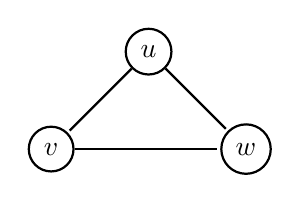
\begin{tikzpicture}[-,>=stealth,shorten >=1pt,auto,node distance=1.75cm, thick,main node/.style={scale=0.9,circle,draw,font=\sffamily\normalsize}]

            \node[circle, draw] (1) []{$u$};
            \node[circle, draw] (2) [below left of = 1]{$v$};
            \node[circle, draw] (3) [below right of = 1]{$w$};

            \draw[-] (1) to (2);
            \draw[-] (1) to (3);
            \draw[-] (2) to (3);

            ;
        \end{tikzpicture}
        \caption{The graph $K_3$.}
    \end{figure}

    it is easy to see that $$\mathrm{IP^*}(K_3) = 1 + 1 = 2$$ because 1 single node is not sufficient to cover all 3 edges in $E(K_3)$. However, since the values in the solution of the LP can be \tit{real-valued}, the value of an optimal solution for the LP relaxation is actually achieved by setting $$\overline x_u = \overline x_v = \overline x_w = \dfrac{1}{2} \implies \mathrm{LP}^*(K_3) = 3 \cdot \dfrac{1}{2} = \dfrac{3}{2}$$ therefore, by definition of IG we have that $$\exists I \in \mathrm P \quad \mathrm{IG_{VC}}(I) := \dfrac{\mathrm{IP^*_{VC}}(K_3)}{\mathrm{LP^*_{VC}}(K_3)} = \dfrac{2}{\tfrac{3}{2}} = \dfrac{4}{3} \implies \mathrm{IG_{VC}} := \sup_{I \in \mathrm P}{\dfrac{\mathrm{IP^*_{VC}}(I)}{\mathrm{LP^*_{VC}}(I)}} \ge \dfrac{4}{3}$$ 

    Moreover, \cref{lp 2-approx vc} shows that we already know an algorithm that employs LP relaxation which yields a 2-approximation of VC; therefore, this lower bound on $\mathrm{IG_{VC}}$ --- together with the previous proposition --- implies that any possible approximation ratio $\alpha$ on VC must satisfy $$2 \ge \alpha \ge \mathrm{IG_{VC}} \ge \dfrac{4}{3}$$ The following theorem proves that we can actually bound $\mathrm{IG_{VC}}$ tightly.

    \begin{framedthm}{Integrality gap for VC}
        $\mathrm{IG_{VC}} = 2$
    \end{framedthm}

    \begin{proof}
        We already proved that the upper bound is 2, so we just need to prove that the lower bound is 2 as well.

        Consider a clique $K_n$; by the same reasoning presented for the case of $K_3$, a feasible solution for the LP relaxation over this graph would be $$x_1 = \ldots = x_n = \dfrac{1}{2} \implies \mathrm{LP^*}(K_n) \le n \cdot \dfrac{1}{2} = \dfrac{n}{2}$$

        \claim{
            Any minimum vertex cover of $K_n$ has exactly $n - 1$ vertices.
        }{
            Consider a $K_n$ with vertices $V(K_n) = \{v_1, \ldots, v_n\}$, and let $S = \{v_1, \ldots, v_{n - 1}\}$ be a set of its vertices. We observe that

            \begin{itemize}
                \item for each edge $\{v_i, v_j\} \in E(K_n)$ such that $i, j \in [n - 1]$, clearly $S$ covers the edge
                \item for each edge $\{v_i, v_n\} \in E(K_n)$, we observe that $v_I \in S$, therefore $S$ still covers the edge
            \end{itemize}

            This concludes that $n - 1$ vertices are \tit{suffice} to cover $V(K_n)$.

            Now, by way of contradiction suppose that there is a vertex cover $S'$ of $K_n$ such that $\abs{S'} \le n - 2$. This implies that there are two vertices $u, v \in V(K_n) - S'$. However, this implies that the edge $\{u, v\} \in E(K_n)$ is not covered --- and such always exists since $K_n$ is a complete graph $\lightning$. This proves that $n - 1$ vertices are \tit{needed}.
        }

        This claim shows that for any $n$ it holds that $\mathrm{IP^*}(K_n) = n - 1$, therefore we have that $$\mathrm{IG}(K_n) = \dfrac{\mathrm{IP^*}(K_n)}{\mathrm{LP^*}(K_n)} \ge \dfrac{n - 1}{\tfrac{n}{2}}$$ which means that $$\mathrm{IG_{VC}} = \sup_{I \in \mathrm{VC}}{\mathrm{IG_{VC}}(I)} \ge \lim_{n \to +\infty}{\dfrac{n - 1}{\tfrac{n}{2}}} = 2$$
    \end{proof}

    \subsection{The Set Cover problem}

    The next problem that we will study can be seen as a \tit{generalization} of the VC problem, which is the \href{https://en.wikipedia.org/wiki/Set_cover_problem}{Set Cover} problem, defined as follows.

    \begin{frameddefn}{Set Cover problem}
        The \tbf{Set Cover} (SC) problem is defined as follows: given a \tit{universe} (or \tit{ground}) set $\mathcal U = [n]$, and a collection of sets $C = \{S_1, \ldots, S_m\}$ such that $S_i \subseteq \mathcal U$, determine the smallest sub-collection $S \subseteq C$ such that $\bigcup_{S_j \in S}{S_j} = \mathcal U$.
    \end{frameddefn}

    In other words, we are asked to determine the smallest sub-collection of the given $C$ such that we can still cover the whole universe set $\mathcal U$. For instance, given $\mathcal U = [3]$ and $S_1 = \{1, 2\}$, $S_2 = \{2, 3\}$, $S_3 = \{1, 3\}$, we can cover $\mathcal U$ with just $S = \{S_1, S_2\}$.

    As for VC, in 1972 \cite{karp} proved that SC is \NPclass-complete as well. Moreover, similarly to what we did for VC, we can convert SC into an IP, as follows.

    \begin{figure}[H]
        \centering
        \[\begin{array}{ccl}
            \qquad\qquad\quad
            & \min \; \displaystyle \sum_{j = 1}^m {x_j} \\\\
            & \sum\limits_{\substack{j \in [m] : \\ i \in S_j}}{x_j} \ge 1 & \forall i \in [n] \\
            & x_j \in \{0, 1\} & \forall j \in [m]
        \end{array}\]
        \caption{IP for SC.}
    \end{figure}

    The first constraint of the IP states that, given an element $i$ in the universe set, at least one of the variables $x_j$ --- representing the sets $S_j$ --- which contain $i$, must be set to 1. In other words, we are guaranteeing that all the elements $i \in \mathcal U$ are covered by at least one set of $C$. Lastly, we want to minimize over the size of the sub-collection of $C$, hence the objective function.

    The LP relaxation that we will consider is the same that we defined for VC. However, differently from VC, the \tit{rounding rule} that we applied to obtain an integral solution --- namely by defining $$S = \{v \in V \mid x_v \ge \tfrac{1}{2}\}$$ cannot be applied for this problem. For instance, say that some element $i \in \mathcal U$ is contained in 3 sets $S_1$, $S_2$ and $S_3$; hence, the second constraint forces the solution of the LP to satisfy $$x_1 + x_2 + x_3 \ge 1$$ Nevertheless, by setting $$x_1 = x_2 = x_3 = \dfrac{1}{3}$$ we would get a feasible solution for the LP relaxation, but then our rounding rule would return an empty set $S = \varnothing$, which is not a feasible solution for our instance of SC since $i$ would not be covered.

    To fix this issue, we are going to present a \tbf{randomized rounding algorithm}, which surprisingly seem to be the \tit{best} approach to perform rounding on LP relaxation solutions that we have at our disposal.

    \begin{framedalgo}{Randomized rounding for SC}
        Given an instance $(\mathcal U, C)$ of SC, the algorithm returns a set cover $A$ for $\mathcal U$. \\
        \hrule

        \quad
        \begin{algorithmic}[1]
            \Function{RandomizedRoundingSC}{$\mathcal U$, $C$}
                \State $A := \varnothing$
                \State $\{\overline x_j\}_{j \in [m]} := \mathrm{LP_{SC}}(\mathcal U, C)$ \Comment{an optimal soluion on the LP relaxation}
                \For{$k \in \sbk{\ceil{2 \ln n}}$}
                    \For{$j \in [m]$}
                        \State Let $c_{k, j}$ be the outcome of the flip of an ind. coin with H prob. set to $\overline x_j$
                        \If{$c_{k, j} == \mathrm H$}
                            \State $A = A \cup \{S_j\}$
                        \EndIf
                    \EndFor
                \EndFor
            \EndFunction
        \end{algorithmic}
    \end{framedalgo}

    First, we are going to prove that the output $A$ of this algorithm is indeed a set cover, with enough probability.

    \begin{framedlem}{}
        Let $(\mathcal U, C)$ be a SC instance, and let $A = \textsc{RandomizedRoundingSC}(\mathcal U, C)$. Then, it holds that $$\Pr[A \ \mathrm{is \ a \ set \ cover}] \ge 1 - \dfrac{1}{n}$$
    \end{framedlem}

    \begin{proof}
        Each iteration of the outermost \ttt{for} loop will be referred to as \tit{phase}.

        \claim[Claim 1]{
            The element $i$ is covered by $A$ in \tit{phase} $k$ with probability at least $1 - \frac{1}{e}$.
        }{
            \begin{equation*}
                \begin{alignedat}{2}
                    \Pr[i \ \mathrm{is \ not \ covered \ in \ \mathit{phase}} \ k] &= \prod_{\substack{j \in [m]: \\ i \in S_j}}{(1 - \overline x_j)} && \quad \quad (\mathrm{the \ prob. \ of \ T}) \\
                                                                                   &\le \prod_{\substack{j \in [m] : \\ i \in S_j}}{e^{-\overline x_j}} && \quad \quad (1 - x \le e^{-x})  \\
                                                                                   &= e^{\displaystyle - \sum\limits_{\substack{j \in [m]: \\ i \in S_j}}{\overline x_j}} && \\
                                                                                   &\le e^{-1} && \quad \quad (\mathrm{second \ constraint \ of \ the \ LP}) \\
                                                                                   &=\dfrac{1}{e} && \\
                \end{alignedat}
            \end{equation*}
        }

        \claim[Claim 2]{
            The element $i$ is not covered by any set of $A$ with probability at most $\frac{1}{n^2}$.
        }{
            \begin{equation*}
                \begin{alignedat}{2}
                    \Pr[i \ \mathrm{is \ not \ covered \ by \ any \ set \ of} \ A] &= \prod_{k = 1}^{\ceil{2 \ln n}}{\Pr[i \ \mathrm{is \ not \ covered \ in \ \mathit{phase}} \ k]} && \\
                                                                                   &\le \prod_{k = 1}^{\ceil{2 \ln n}}{\dfrac{1}{e}} && \quad \quad (\mathrm{by \ Claim \ 1}) \\
                                                                                   &= e^{- \ceil {2 \ln n }} && \\
                                                                                   &\le e^{- 2 \ln n} && \\
                                                                                   &= \dfrac{1}{n^2} && \\
                \end{alignedat}
            \end{equation*}
        }

        \claim[Claim 3]{
            $A$ is a set cover with probability at least $1 - \frac{1}{n}$.
        }{
            \begin{equation*}
                \begin{alignedat}{2}
                    \Pr[A \ \mathrm{is \ not \ a \ set \ cover}] &= \Pr[\exists i \quad i \ \mathrm{is \ not \ covered \ by \ any \ set \ of} \ A] && \\
                                                                 &\le \sum_{i = 1}^n{\Pr[i \ \mathrm{is \ not \ covered \ by \ any \ set \ of} \ A]} && \\
                                                                 &\le \sum_{i = 1}^n{\dfrac{1}{n^2}} && \quad \quad (\mathrm{by \ Claim \ 2}) \\
                                                                 &= \dfrac{n}{n^2} && \\
                                                                 &= \dfrac{1}{n} && \\
                \end{alignedat}
            \end{equation*}
        }

        The statement follows directly from Claim 3.
    \end{proof}

    Next, we will show that this algorithm yields \tit{on average} a $\ceil{2 \ln n}$-approximation of SC.

    \begin{framedlem}{}
        Let $(\mathcal U, C)$ be a SC instance, and let $A = \textsc{RandomizedRoundingSC}(\mathcal U, C)$. Then, it holds that $$\mathbb E \sbk{\abs A} \le \ceil{2 \ln n} \mathrm{IP}^*$$
    \end{framedlem}

    \begin{proof}
        Fix a \tit{phase} $k$, and let $A_k$ be the collection of sets added to $A$ at \tit{phase} $k$; then it holds that $$\mathbb E \sbk{\abs{A_k}} = \sum_{j = 1}^m {1 \cdot \Pr[S_j \in A_k]} = \sum_{j = 1}^m{\overline x_j} = \mathrm{LP^*}$$ Moreover, since $\displaystyle A = \bigcup_{k \in \ceil{2 \ln n}}{A_k}$, we have that $$\mathbb E \sbk{\abs A} \le \mathbb E \sbk{\sum_{k \in \ceil{2 \ln n}}{\abs{A_k}}} = \sum_{k \in \ceil {2 \ln n}}{\mathbb E \sbk{\abs{A_k}}} = \sum_{k \in \ceil{2 \ln n}}{\mathrm{LP^*}} = \ceil{2 \ln n} \mathrm{LP^*} \le \ceil{2 \ln n} \mathrm{IP^*}$$
    \end{proof}

    By the law of large numbers, we know that if for each pair $(\mathcal U, C)$ we repeatedly compute the previous algorithm we will, eventually, get an output $A'$ such that $\abs{A'} \le \ceil{2 \ln n} \mathrm{IP}^*$. This implies that such procedure yield an approximation ratio $\alpha \le \ceil{2 \ln n}$, implying that $$\ceil{2 \ln n } \ge \alpha \ge \mathrm{IG}_{\mathrm{SC}}$$ directly providing an upper bound for SC.

    Additionally, we observe that the algorithm can be modified to get a better bound, by simply replacing $\ceil{2 \ln n}$ with $\ceil{(1 + \varepsilon) \ln n}$, for any $\varepsilon > 0$. In fact, with this modification we would get that $\mathbb E \sbk{\abs A} \le \ceil{(1 + \varepsilon) \ln n} \mathrm{LP^*}$, even though we would also have that $\Pr[\mbox{$\mathcal U$ covered by $A$}] = 1 - n^{- \varepsilon}$ which is worse for small values of $\varepsilon$ --- this probability can still be \tit{boosted} by repeatedly computing the output. Hence, we actually get that $$\mathrm{IG}_{\mathrm{SC}} \le \ceil{\ln n}$$

    With VC we were able to provide a tight bound on $\mathrm{IG_{VC}}$; for SC instead, even though the value of $\mathrm{IG_{SC}}$ is known \cite{ig_sc}, the proof is very complex and we will only show a lower bound.

    \begin{framedthm}{Integrality gap of SC}
        For any $n \in \N$, it holds that $$\dfrac{1}{4 \ln 2} \le \mathrm{IG_{SC}} \le \ceil{\ln n}$$
    \end{framedthm}
    
    \begin{proof}
        We already proved the upper bound, so we just need to prove the lower bound. Furthermore, as shown with VC in the previous section, to provide a lower bound on $\mathrm{IG_{SC}}$ it suffices to show an instance of SC for which the bound holds.

        Let $m \ge 2$ be an even integer, and define the following instance of SC: set $$\mathcal U_m := \{e_A \mid A \subseteq [m] \land \abs A  = \tfrac{m}{2}\} \implies n = \abs{\mathcal U_m}= \binom{m}{\tfrac{m}{2}}$$ and define the collection of sets as follows $$\forall j \in [m] \quad S_j := \{e_A \mid e_A \in \mathcal U_m \land j \in A\}$$ and set $C_m := \{S_1, \ldots, S_m\}$ For example, if $m = 4$ we have that $$\mathcal U_4 := \{e_A \mid A \subseteq \{1, 2, 3, 4\} \land \abs A = \tfrac{4}{2} = 2\} = \{e_{\{1, 2\}}, e_{\{1, 3\}}, e_{\{1, 4\}}, e_{\{2, 3\}}, e_{\{2, 4\}}, e_{\{3, 4\}}\}$$ $$S_1 := \{e_{\{1,2\}}, e_{\{1, 3\}}, e_{\{1,4\}}\}$$ $$S_2 := \{e_{\{1, 2\}}, e_{\{2, 3\}}, e_{\{2,4\}}\}$$ $$S_3 := \{e_{\{1, 3\}}, e_{\{2, 3\}}, e_{\{3, 4\}}\}$$ $$S_4 := \{e_{\{1, 4\}}, e_{\{2, 4\}}, e_{\{3, 4\}}\}$$

        Note that, thanks to \href{https://en.wikipedia.org/wiki/Stirling%27s_approximation}{Stirling's approximation} we know that $$n = \binom{m}{\tfrac{m}{2}} = \Theta \rbk{\dfrac{2^m}{\sqrt m}} \implies m = \log n - \Theta(\log \log n)$$

        \claim{
            $\forall m \ge 2 \ \mathrm{even} \quad \mathrm{LP^*_{SC}}(\mathcal U_m, C_m) \le 2$.
        }{
            Consider the solution $$x_1 = \ldots = x_m = \dfrac{2}{m}$$ for the LP relaxation; clearly, $m \ge 2$ therefore $\forall j \in [m] \quad 0 \le x_j \le 1$, and $$\forall e_A \in \mathcal U \quad \sum_{\substack{j \in [m]: \\ e_A \in S_j}}{x_j} = \sum_{\substack{j \in [m]: \\ e_A \in S_j}}{\dfrac{2}{m}} = \abs A \cdot \dfrac{2}{m} = \dfrac{m}{2} \cdot \dfrac{2}{m} = 1 \ge 1$$ hence this is a feasible solution to the LP, and its value is simply given by $m \cdot \frac{2}{m} = 2$.
        }

        \claim{
            $\forall m \ge 2 \ \mathrm{even} \quad \mathrm{IP^*}(\mathcal U_m, C_m) \ge \tfrac{1}{2} \log n - O(\log \log n)$.
        }{
            By way of contradiction, assume that there exists a sub-collection $S = \{S_{i_1}, \ldots, S_{i_k}\} \subseteq C_m$ with $k \le \tfrac{m}{2}$ that covers $\mathcal U_m$. Consider the following set $$T := [m]- \{i_1, \ldots, i_k\}$$ thus, we have that $$\abs T \ge m - \dfrac{m}{2} = \dfrac{m}{2}$$ hence, we can always define a subset $A \subseteq T$ such that $\abs A = \tfrac{m}{2}$. However, we observe that $$A \subseteq T \implies i_1, \ldots, i_k \notin A \implies e_A \notin S_{i_1} \cup \ldots \cup S_{i_k}$$ hence $e_A$ is not covered by $S$ $\lightning$.

            This means that for any set cover $S$ of $(\mathcal U_m, C_m)$ it must hold that $$\abs S > \dfrac{m}{2} = \dfrac{1}{2} \log n - \Theta(\log \log n) \implies \mathrm{IP^*}(\mathcal U_m, C_m) \ge \dfrac{m}{2} = \dfrac{1}{2} \log n - O(\log \log n)$$
        }

        Finally, from these two claims, it follows that $$\mathrm{IG_{SC}}(\mathcal U_m, C_m) = \dfrac{\mathrm{IP^*}(\mathcal U_m, C_m)}{\mathrm{LP^*}(\mathcal U_m, C_m)} \ge \dfrac{\tfrac{1}{2} \log n - O(\log \log n)}{2} = \dfrac{1}{4} \log n - O(\log \log n)$$ which means that $$\mathrm{IG_{SC}} = \sup_{I \in \mathrm{SC}}{\mathrm{IG_{SC}}(I)} \ge \mathrm{IG_{SC}}(\mathcal U_m, C_m) \ge \dfrac{1}{4} \log n = \dfrac{1}{4 \ln 2} \ln n$$
    \end{proof}

    \subsection{The Densest Subgraph problem}
    
    Up to this point, we only discussed \NPclass-complete problems, and various techniques used to obtain approximate solutions. The next problem that we are going to introduce, instead, can be solved in \tbf{polynomial} time, thanks to linear programming. First, consider the following definition.

    \begin{frameddefn}{Graph density}
        Given a graph $G = (V, E)$ such that $V \neq \varnothing$, its \tbf{density} is defined as follows $$\rho(G) := \dfrac{\abs E}{\abs V}$$
    \end{frameddefn}

    Note that we require $V \neq \varnothing$, but we will omit this detail in the following sections.

    For instance, the density of the graph $G = (V, E)$ below

    \begin{figure}[H]
        \centering
        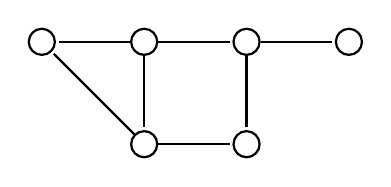
\begin{tikzpicture}[-,>=stealth,shorten >=1pt,auto,node distance=1.3cm, thick,main node/.style={scale=0.9,circle,draw,font=\sffamily\normalsize}]

            \node[circle, draw] (1) []{};
            \node[circle, draw] (2) [right of = 1]{};
            \node[circle, draw] (3) [below of = 1]{};
            \node[circle, draw] (4) [below of = 2]{};
            \node[circle, draw] (5) [left of = 1]{};
            \node[circle, draw] (6) [right of = 2]{};

            \draw[-] (1) to (2);
            \draw[-] (1) to (3);
            \draw[-] (2) to (4);
            \draw[-] (1) to (5);
            \draw[-] (3) to (4);
            \draw[-] (3) to (5);
            \draw[-] (2) to (6);

            ;
        \end{tikzpicture}
        % \caption{An example of a vertex cover.}
    \end{figure}

    is evaluated through the following ratio $$\rho(G) := \dfrac{\abs E}{\abs V} = \dfrac{7}{6} = 1.1 \overline 6$$ The problem that we are going to introduce is the following.

    \begin{frameddefn}{Densest Subgraph problem}
        The \tbf{Densest Subgraph} (DS) problem is defined as follows: given an undirected graph $G = (V, E)$, determine the induced subgraph of $G$ that maximizes its density. In other words, the problem asks to find a set of vertices $S^*$ in $$S^* \in \argmax_{S \subseteq V}{\rho(G[S])}$$
    \end{frameddefn}

    \begin{figure}[H]
        \centering
        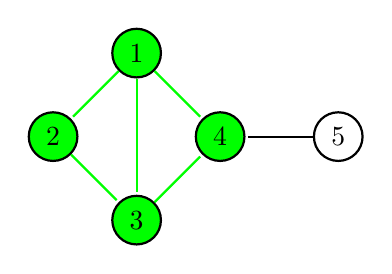
\begin{tikzpicture}[-,>=stealth,shorten >=1pt,auto,node distance=1.5cm, thick,main node/.style={scale=0.9,circle,draw,font=\sffamily\normalsize}]

            \node[circle, draw, fill=green] (1) []{1};
            \node[circle, draw, fill=green] (2) [below left of = 1]{2};
            \node[circle, draw, fill=green] (3) [below right of = 2]{3};
            \node[circle, draw, fill=green] (4) [below right of = 1]{4};
            \node[circle, draw] (5) [right of = 4]{5};

            \draw[-] (1) [green] to (2);
            \draw[-] (2) [green] to (3);
            \draw[-] (3) [green] to (4);
            \draw[-] (1) [green] to (4);
            \draw[-] (1) [green] to (3);
            \draw[-] (5) to (4);

            ;
        \end{tikzpicture}
        \caption{For instance, in this graph the set $S$ that maximizes $\rho(G[S])$ is given by $S = \{1, 2, 3, 4\}$, which yields a density of $\tfrac{5}{4} = 1.25$.}
    \end{figure}

    The densest subgraph is relevant because it actually \tit{maximizes} the average degree of its vertices. In fact, thanks to the handshaking lemma we have that $$\rho(G[S]) := \dfrac{\abs{E(G[S])}}{\abs S} = \dfrac{1}{2} \cdot \dfrac{2 \cdot \abs{E(G[S])}}{\abs s} = \dfrac{1}{2} \cdot \dfrac{\sum_{v \in S}{\deg (v)}}{\abs S} = \dfrac{1}{2} \avg_{v \in S}{\deg(v)}$$

    The LP that we will present for this problem is the following. However, to show that this LP actually yields a solution for DS is not trivial, and it will be proven through the following theorems.

    \begin{figure}[H]
        \centering
        \[\begin{array}{ccl}
            \qquad\qquad\quad
            & \max \; \displaystyle \sum_{e \in E} {x_e} \\\\
            & x_{ij} \le y_i & \forall i j \in E \\
            & x_{ij} \le y_j & \forall i j \in E \\
            & \sum\limits_{i \in V}{y_i} \le 1 \\
            & x_{ij} \ge 0 & \forall i j \in E \\
            & y_i \ge 0 & \forall i \in V \\
        \end{array}\]
        \caption{LP for DS.}
        \label{ds lp}
    \end{figure}

    \begin{framedlem}{}
        Given a graph $G = (V, E)$, for any $S \subseteq V$ there exists a feasible solution $\{x_e, y_i\}_{e \in E, i \in V}$ to the LP having value at least $\rho(G[S])$.
    \end{framedlem}

    \begin{proof}
        Given a set $S \subseteq V$, construct the following solution:

        \begin{itemize}
            \item $\forall ij \in E \quad x_{ij} := \soe{ll}{\dfrac{1}{\abs S} & i, j \in S \\ 0 & i \notin S \lor j \notin S}$
            \item $\forall i \in V \quad y_i := \soe{ll}{\dfrac{1}{\abs S} & i \in S \\ 0 & i \in V - S}$
        \end{itemize}

        We observe that

        \begin{itemize}
            \item $ij \in E(G[S]) \implies i, j \in S \implies \soe{l}{x_{ij} = \dfrac{1}{\abs S} \\ y_i = y_j = \dfrac{1}{\abs S}} \implies x_ij \le y_i, y_j$
            \item $ij \notin E(G[S]) \implies i \notin S \lor j \notin S \implies x_{ij} = 0$, but since $y_i, y_j \ge 0$ for any $i, j \in V$ by definition, it holds that $x_{ij} \le y_i, y_j$
        \end{itemize}

        Additionally, notice that $$\sum_{i \in V}{y_i} = \sum_{i \in S}{y_i} + \sum_{i \in V - S}{y_i} = \abs S \cdot \dfrac{1}{\abs S} + \abs {V - S} \cdot 0 = 1 \le 1$$

        This proves that this is a feasible solution to the LP. Lastly, the value of this solution is simply given by $$\sum_{e \in E}{x_e} = \sum_{e \in E(G[S])}{e} + \sum_{e \notin E(G[S])}{x_e} = \abs{E(G[S])} \cdot \dfrac{1}{\abs S} + \abs{E - E(G [S])} \cdot 0 = \dfrac{\abs{E(G[S])}}{\abs S} =: \rho(G[S])$$
    \end{proof}

    In particular, this lemma proves that if $S^*$ is an optimal solution for DS on a graph $G$, then there is a solution to this LP such that $\mathrm{LP^*} \ge \rho(G[S^*])$. The next theorem will prove that $\mathrm{LP^*} \le \rho(G[S^*])$ holds as well, which implies that our LP does in fact produce an optimal solution to DS, and that $\mathrm{IG_{DS}} = 1$.

    \begin{framedthm}{}
        Given a graph $G = (V, E)$, for any $\{x_e, y_i\}_{e \in E, i \in V}$ feasible solution to the LP that has value $v$, there exists a set $S \subseteq V$ such that $\rho(G[S]) \ge v$.
    \end{framedthm}

    \begin{proof}
        Consider a feasible solution $\{x_e', y_i'\}_{e \in E, i \in V}$ of the LP, having value $v$. We will construct another solution to the LP $\{x_e, y_i\}_{e \in E, i \in V}$ starting from the previous solution, as follows:

        \begin{itemize}
            \item $\forall i \in V \quad y_i := y_i'$
            \item $\forall ij \in E \quad x_{ij} := \min(y_i, y_j)$
        \end{itemize}

        It is easy to see that this is a feasible solution to the LP, in fact $$\forall ij \in E \quad x_{ij} := \min(y_i, y_j) \le y_i, y_j$$ and additionally, by feasibility of $\{x_e', y_i'\}_{e \in E, i \in V}$, we have that $$\sum_{i \in V}{y_i} = \sum_{i \in V}{y_i'} \le 1$$ Furthermore, note that $$v = \sum_{e \in E}{x_e'} \le \sum_{e \in E}{\min(y_i', y_j')} = \sum_{e \in E}{\min(y_i, y_j)} = \sum_{e \in E}{x_e}$$ meaning that the value of this solution is at least $v$, but it may be better --- this happens if $x_{ij} < y_i$ or $x_{ij} < y_j$ for some $ij \in E$, and if this is the case we say that there is some \tit{slack}.

        Next, we will construct a series of sets of vertices starting from this new LP solution we just defined. In particular, given a value $r \ge 0$, let $$S(r) := \{i \mid y_i \ge r\}$$ $$E(r) := \{e \mid x_e \ge r\}$$ Notice that $ij \in E(r) \iff i, j \in S(r)$, because $$ij \in E(r) \iff x_{ij} \ge r \iff \min(y_i, y_j) \ge r \iff y_i, y_j \ge r \iff i,j \in S(r)$$ which means that $S(r)$ and $E(r)$ are well-defined --- note that $E(G[S(r)]) = E(r)$.

        \claim{
            There exists a value $r^* \ge 0$ such that $\rho(G[S(r^*)]) \ge v$.
        }{
            Consider the solution $\{x_e, y_i\}_{e \in E, i \in V}$ to the LP that we constructed previously, and let $\pi$ be the permutation of the $y_i$'s such that $$0 \le y_{\pi (1)} \le y_{\pi (2)} \le \ldots \le y_{\pi(n - 1)} \le y_{\pi (n)}$$ which means that $\pi$ defines a sorting of the $y_i$'s. Now, consider the possible values of $r \ge 0$, and what happens inside $S(r)$:

            \begin{itemize}
                \item for $r = 0$, by feasibility of our solution we have that $$S(r) = S(0) := \{i \mid y_i \ge 0\} \implies \abs{S(r)} = n$$
                \item notice that for any value $0 \le r \le y_{\pi (1)} \le \ldots \le y_{\pi (n)}$, the value of $\abs{S(r)}$ will still be $n$, by its definition
                \item however, if $0 \le y_{\pi (1)} < r \le \ldots \le y_{\pi (n)}$, then the vertex $\pi(1)$ will be the only verterx not contained in $S(r)$, therefore $\abs{S(r)} = n - 1$
            \end{itemize}

            Repeating the same argument for all the possible values of $r$, we obtain the following graph for $\abs{S(r)}$.

            \begin{figure}[H]
                \centering
                \begin{tikzpicture}[scale=0.7]
                    \draw[-stealth] (-0.5,0) -- (2,0) node[below]{$y_{\pi(1)}$} -- (4,0) node[below]{$y_{\pi(2)}$} -- (7,0) node[below]{$\cdots$} -- (10,0) node[below]{$y_{\pi(n - 2)}$} -- (12,0) node[below]{$y_{\pi(n - 1)}$} -- (14,0) node[below]{$y_{\pi(n)}$} -- (15,0) node[right]{$r$};
                    \draw[-stealth] (0,-0.5) -- (0,0) node[below left]{0} -- (0,1) node[left]{1} -- (0,2) node[left]{2} -- (0,3.5) node[left]{$\cdots$} -- (0,5) node[left]{$n - 1$} -- (0,6) node[left]{$n$} -- (0,7.5) node[above]{$\abs{S(r)}$};
                    \draw[thick, orange] (0,6) -- (2,6) -- (2,5) -- (4,5) -- (4, 4) -- (5,4);
                    \draw[dashed, orange] (5,4) -- (6,4);
                    \draw[dashed, orange] (9,3) -- (8,3);
                    \draw[thick, orange] (14,0) -- (14,1) -- (12,1) -- (12,2) -- (10,2) -- (10,3) -- (9,3);
                \end{tikzpicture}
            \end{figure}

            From this graph, it is easy to see that computing the integral of $\abs{S(r)}$ is trivial, because
            \begin{equation*}
                \begin{split}
                    \int_{0}^{y_{\pi(n)}}{\abs{S(r)} \, d r} &= \int_{0}^{y_{\pi(1)}}{\abs{S(r)} \, dr} + \int_{y_{\pi(1)}}^{y_{\pi(2)}}{\abs{S(r)} \, dr} + \ldots + \int_{y_{\pi(n -1)}}^{y_{\pi(n)}}{\abs{S(r)} \, dr} \\
                                                             &= \int_{0}^{y_{\pi(1)}}{n \, dr} + \int_{y_{\pi(1)}}^{y_{\pi(2)}}{(n - 1) \, dr} + \ldots + \int_{y_{\pi(n - 1)}}^{y_{\pi(n)}}{1 \, dr} \\
                                                             &= n \cdot (y_{\pi(1)} - 0) + (n - 1) \cdot(y_{\pi(2)} - y_{\pi(1)}) + \ldots + 1 \cdot (y_{\pi(n)} - y_{\pi(n - 1)}) \\
                                                             &= y_{\pi(1)} \cdot\sbk{n - (n - 1)} + y_{\pi(2)}\cdot \sbk{(n - 1) - (n - 2)} + \ldots + y_{\pi(n)}\cdot (1 - 0) \\
                                                             &= y_{\pi(1)} \cdot 1 + y_{\pi(2)} \cdot 1 + \ldots + y_{\pi(n)} \cdot 1 \\
                                                             &= \sum_{i = 1}^n{y_{\pi(i)}} \\
                                                             &= \sum_{i \in V}{y_i} \\
                                                             &\le 1 \quad\quad (\mathrm{by \ feasibility \ of \ the \ solution})
                \end{split}
            \end{equation*}

            By the same argument, we can derive that $$\int_0^{y_{\pi(n)}}{\abs{E(r)} \, dr} = \sum_{e \in E}{x_e} \ge v$$ Note that the last inequality was proved before the claim.

            Lastly, we will prove the statement of the claim by way of contradiction. In particular, suppose that for all $r \ge 0$ it holds that $\rho(G[S(r)]) < v$. We can rewrite this inequality as follows $$\rho(G[S(r)]) := \dfrac{\abs{E(r)}}{\abs{S(r)}} < v \iff \abs{E(r)} < v \cdot \abs{S(r)}$$ This inequality can be used to upper bound the integral of $\abs{E(r)}$ \tit{point-by-point}, i.e. $$v \le \int_0^{y_{\pi(n - 1)}}{\abs{E(r)} \, dr} < \int_0^{y_{\pi(n - 1)}}{v \cdot \abs{S(r)} \, dr} = v \cdot \int_0^{y_{\pi(n - 1)}}{\abs{S(r)} \, dr} \le v \cdot 1 = v$$ meaning that $v < v$ $\lightning$.
        }

        Finally, since we proved that $G[S(r)]$ is well-defined, and this claim proves that there exists an $r^*$ such that $\rho(G[S(r^*)]) \ge v$, the statement holds.
    \end{proof}

    \subsection{Approximation through duality}

    As we discussed at the beginning of this section, the cost of solving an LP generally depends on the number of \tit{variables} and \tit{constraints} it has. In particular, the LP we presented for solving DS has a \tit{large} number of both, which means that while the cost remains \tit{polynomial}, the degree of the polynomial is too high, making this approach \tbf{impractical} for large graphs.

    Now, we are going to present a \tbf{greedy algorithm}, developed by \textcite{charikar} in 2000, and we will prove that this algorithm yields a $\tfrac{1}{2}$-approximation of DS.

    \begin{framedalgo}[label={charikar's algo}]{Charikar's algorithm}
        Given an undirected graph $G = (V, E)$, the algorithm returns a $\tfrac{1}{2}$-approximation solution of DS on $G$. \\
        \hrule

        \quad
        \begin{algorithmic}[1]
            \Function{Charikar}{$G$}
                \State $S_0 := V(G)$
                \For{$i \in [n - 1]$}
                    \State $\displaystyle v_i \in \argmin_{v \in S_{i - 1}}{\deg_{G[S_{i - 1}]}(v)}$
                    \State $S_i := S_{i - 1} - \{v_i\}$
                \EndFor
                \State \textbf{return} $\displaystyle S^* \in \argmax_{i \in [0, n - 1]}{\rho(G[S_i])}$
            \EndFunction
        \end{algorithmic}
    \end{framedalgo}

    \idea{
        The algorithm constructs a series $S_0, \ldots, S_n$ of sets of vertices, such that $\abs{S_i} = n - i$, and at each iteration the $i$-th vertex that gets removed from $G[S_{i - 1}]$ is the one having minimum degree. At the end, the algorithm returns the set $S^*$ that maximizes the density of $G[S^*]$.
    }

    We observe that this algorithm does not return an optimal solution in general; in particular, problems can arise if there are vertices of equal degree. For instance, consider the following disconnected graph

    \begin{figure}[H]
        \centering
        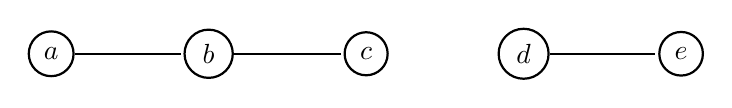
\begin{tikzpicture}[-,>=stealth,shorten >=1pt,auto,node distance=2cm, thick,main node/.style={scale=0.9,circle,draw,font=\sffamily\normalsize}]

            \node[circle, draw] (1) []{$a$};
            \node[circle, draw] (2) [right of = 1]{$b$};
            \node[circle, draw] (3) [right of = 2]{$c$};
            \node[circle, draw] (4) [right of = 3]{$d$};
            \node[circle, draw] (5) [right of = 4]{$e$};

            % \path[every node/.style={font=\sffamily\small}]

            \draw[-] (1) to (2);
            \draw[-] (2) to (3);
            \draw[-] (4) to (5);

            ;
        \end{tikzpicture}
    \end{figure}

    In this graph, the densest subgraph is induced by the set $S^* = \{a, b, c\}$, because $$\rho(G[S^*]) = \dfrac{2}{3}$$ However, since $\deg(a) = \deg(c) = \deg(d) = \deg(e) = 1$, the algorithm may choose $v_1 := a$, meaning that $G[S_1]$ would be 

    \begin{figure}[H]
        \centering
        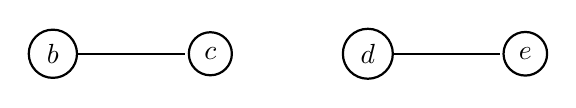
\begin{tikzpicture}[-,>=stealth,shorten >=1pt,auto,node distance=2cm, thick,main node/.style={scale=0.9,circle,draw,font=\sffamily\normalsize}]

            \node[circle, draw] (2) []{$b$};
            \node[circle, draw] (3) [right of = 2]{$c$};
            \node[circle, draw] (4) [right of = 3]{$d$};
            \node[circle, draw] (5) [right of = 4]{$e$};

            % \path[every node/.style={font=\sffamily\small}]

            \draw[-] (2) to (3);
            \draw[-] (4) to (5);

            ;
        \end{tikzpicture}
    \end{figure}

    and it is easy to see that $G[S_0] = G$, and any other subgraph of this graph, have lower density than $G[S^*]$.

    To prove that this algorithm yields a $\tfrac{1}{2}$-approximation, we are going to introduce some definitions first.

    \begin{frameddefn}{Orientation}
        Given an undirected graph $G = (V, E)$, an \tbf{orientation} of $G$ is a function $\func{\phi}{E}{V}$ that assigns to each edge $\{u, v\} \in E$ either $u$ or $v$.
    \end{frameddefn}

    Note that, by definition for any $e \in E$ it holds that $\phi(e) \in e$. For instance, given the following graph

    \begin{figure}[H]
        \centering
        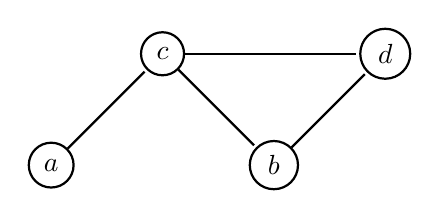
\begin{tikzpicture}[-,>=stealth,shorten >=1pt,auto,node distance=2cm, thick,main node/.style={scale=0.9,circle,draw,font=\sffamily\normalsize}]

            \node[circle, draw]  (1) []{$a$};
            \node[circle, draw]  (2) [above right of = 1]{$c$};
            \node[circle, draw]  (3) [below right of = 2]{$b$};
            \node[circle, draw]  (4) [above right of = 3]{$d$};

            % \path[every node/.style={font=\sffamily\small}]

            \draw[-] (1) to (2);
            \draw[-] (2) to (3);
            \draw[-] (2) to (4);
            \draw[-] (3) to (4);

            ;
        \end{tikzpicture}
        % \caption{Given the set of red vertices $S$, the green edges represent $\mathrm{cut}(S)$.}
    \end{figure}

    and the following function $\phi$

    \begin{center}
        \begin{tabular}{c|c c} 
             \hline
             $e$ & $\phi(e)$ \\
             \hline\hline
             $ac$ & $c$ \\ 
             \hline
             $bc$ & $c$ \\
             \hline
             $bd$ & $b$ \\
             \hline
             $cd$ & $d$ \\
             \hline
        \end{tabular}
    \end{center}

    we would get the following orientation on $G$

    \begin{figure}[H]
        \centering
        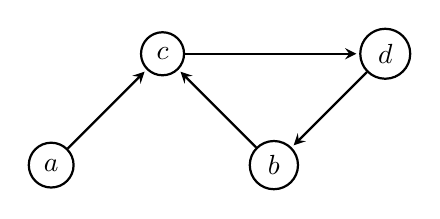
\begin{tikzpicture}[-,>=stealth,shorten >=1pt,auto,node distance=2cm, thick,main node/.style={scale=0.9,circle,draw,font=\sffamily\normalsize}]

            \node[circle, draw]  (1) []{$a$};
            \node[circle, draw]  (2) [above right of = 1]{$c$};
            \node[circle, draw]  (3) [below right of = 2]{$b$};
            \node[circle, draw]  (4) [above right of = 3]{$d$};

            % \path[every node/.style={font=\sffamily\small}]

            \draw[->] (1) to (2);
            \draw[->] (3) to (2);
            \draw[->] (2) to (4);
            \draw[->] (4) to (3);

            ;
        \end{tikzpicture}
        \caption{The previous graph, oriented through $\phi$.}
        \label{oriented graph}
    \end{figure}

    Given an orientation $\phi$ of $G$, and a vertex $v \in V(G)$ we will indicate with $\deg_\phi(v)$ the in-degree of $v$ w.r.t. $\phi$, i.e. $$\deg_\phi(v) := \abs{\{e \in E \mid \phi(e) = v\}}$$ For example, in the previous graph we have that $\deg_\phi(c) = 2$, $\deg_\phi(a) = 0$ and $\deg_\phi(b) = \deg_\phi(d) = 1$. By the same argument that proves the handshaking lemma, we observe that $$\sum_{v \in V(G)}{\deg_\phi(v)} = \abs E$$ Lastly, the maximum in-degree w.r.t. $\phi$ will be denoted as $$\Delta_\phi := \max_{v \in V} {\deg_\phi(v)}$$ We are now ready to prove the approximation ratio of Charikar's algorithm.

    \begin{framedthm}[label={charikar approx}]{}
        Given a graph $G$, and an optimal solution $\rho(G[S^*])$ for DS on $G$, let $M := \textsc{Charikar}(G)$; then, it holds that $\tfrac{1}{2} \rho(G[S^*]) \le M$.
    \end{framedthm}

    \begin{proof}
        We are going to prove this approximation ratio through two claims.

        \claim[Claim 1]{
            Given an undirected graph $G$, and an optimal solution $\rho(G[S^*])$ for DS on $G$, for any orientation $\phi$ of $G$ it holds that $\rho(G[S^*]) \le \Delta_\phi$.
        }{
            By definition of $\phi$, each $uv \in E$ is going to be oriented towards either $u$ or $v$, therefore if $uv \in E(G[S^*])$ then $uv$ is going to be oriented towards a node of $S$. Hence, we have that \centeredeq{0.99}{$\displaystyle \abs{E(G[S^*])} \le \sum_{v \in V(G[S^*])}{\deg_\phi(v)} \le \sum_{v \in V(G[S^*])}{\Delta_\phi} = \abs {V[G(S^*)]} \cdot \Delta_\phi \iff \rho(G[S^*]) := \dfrac{\abs{E(G[S^*]})}{\abs{V(G[S^*])}} \le \Delta_\phi$}
        }

        Consider Charikar's algorithm; before proving the second claim, we need to introduce an orientation $\phi_\mathrm{GR}$ --- where GR stands for \tit{greedy} --- of $G$ defined as follows: if $v_i$ is the $i$-th vertex --- removed from $G[S_{i - 1}]$ --- picked by the algorithm, orient any edge $\{u, v_i\} \in E(G)$ towards $v_i$, for any $u \in V(G)$. For instance, Charikar's algorithm applied on the graph shown in \cref{oriented graph} would set $v_1 := a$, therefore $\phi(ca) = a$, and so on. This implies that $$\forall i \in [n] \quad \deg_{G[S_{i - 1}]}(v_i) = \deg_{\phi_\mathrm{GR}}(v_i)$$

        \claim[Claim 2]{
            Given an undirected graph $G$, and $M := \textsc{Charikar}(G)$, it holds that $\Delta_{\phi_\mathrm{GR}} \le 2M$.
        }{
            Observe that for any $i \in [n]$ it holds that $$v_i \in \argmin_{v \in S_{i - 1}}{\deg_{G[S_{i - 1}]}(v)} \iff \deg_{G[S_{i - 1}]}(v_i) = \min_{v \in S_{i - 1}}{\deg_{G[S_{i - 1}]}(v)}$$ therefore, we have that 
            \begin{equation*}
                \begin{split}
                    \deg_{\phi_\mathrm{GR}}(v_i) &= \deg_{G[S_{i - 1}]}(v_i) \\
                                                 &= \min_{v \in S_{i - 1}}{\deg_{G[S_{i - 1}]}(v)} \\
                                                 &\le \avg_{v \in S_{i - 1}}{\deg_{G[S_{i - 1}]}(v)} \\
                                                 &= \dfrac{\displaystyle \sum_{v \in S_{i - 1}}{\deg_{G[S_{i - 1}]}(v)}}{\abs{S_{i - 1}}} \\
                                                 &= \dfrac{2 \abs{E(G[S_{i - 1}])}}{\abs{V(G[S_{i - 1}])}} \\
                                                 &=: 2\rho(G[S_{i - 1}])
                \end{split}
            \end{equation*}
            Finally, we get that
            \begin{equation*}
                \begin{split}
                    \Delta_{\phi_\mathrm{GR}} &:= \max_{v \in V(G)}{\deg_{\phi_\mathrm{GR}}(v)} \\
                                              &= \max_{i \in [n]}{\deg_{\phi_\mathrm{GR}}(v_i)} \\
                                              &\le \max_{i \in [n]}{2 \rho (G[S_{i - 1}])} \quad \quad (\mathrm{for \ the \ previous \ inequality}) \\
                                              &= 2 \max_{i \in [n]}{\rho(G[S_{i - 1}])} \\
                                              &\le 2 \max_{i \in [0, n - 1]}{\rho(G[S_i])} \\
                                              &=: 2M
                \end{split}
            \end{equation*}
        }

        Lastly, putting the two claims together, we get that for any optimal solution $\rho(G[S^*])$ of a given undirected graph $G$, if $M := \textsc{Charikar}(G)$ then $$\rho(G[S^*]) \le \Delta_{\phi_\mathrm{GR}} \le 2M \iff \tfrac{1}{2} \rho(G[S^*]) \le M$$
    \end{proof}

    \section{Approximation through duality}

    In the last proof of the previous section, we defined $\phi_\mathrm{GR}$, which helped us determine the approximation ratio of the algorithm. But how did Charikar come up with such an orientation of the graph? To answer this question, we need to introduce the concept of the \tbf{duality} of linear programs.

    Consider the following \tit{maximization} generic linear program:

    \begin{figure}[H]
        \centering
        \[\begin{array}{cc}
            % \qquad\qquad\quad
            & \max \; c_1x_1 + \ldots + c_n x_n \\\\
            & a_{11}x_1 + \ldots + a_{1n}x_n \le b_1 \\
            & \vdots \\
            & a_{m1}x_1 + \ldots + a_{mn}x_n \le b_m \\
            & x_1, \ldots, x_n \ge 0
        \end{array}\]
        \caption{A \tit{primal} LP.}
    \end{figure}

    As a convention, we will call the \tbf{primal} LP the one that \tit{maximizes} its objective function. Hence, given a primal LP, its \tbf{dual} linear program is defined as follows:

    \begin{figure}[H]
        \centering
        \[\begin{array}{cc}
            % \qquad\qquad\quad
            & \min \; b_1y_1 + \ldots + b_m y_m \\\\
            & a_{11}y_1 + \ldots + a_{m1}y_m \ge c_1 \\
            & \vdots \\
            & a_{1n}y_1 + \ldots + a_{mn}y_m \ge c_n \\
            & y_1, \ldots, y_m \ge 0
        \end{array}\]
        \caption{The \tit{dual} of a primal LP.}
    \end{figure}

    In other words, given a matrix $A \in \R^{m \times n}$, two vectors $c, x \in \R^n$, and two vectors $b, y \in \R^m$, these two programs can be rewritten as follows:
     \begin{figure}[H]
        \centering

        \begin{tabular}{ccccc}
            $\begin{array}{cc}
                % \qquad\qquad\quad
                & \mathrm{\underline{Primal \ LP}} \\\\
                & \max \; c^Tx \\\\
                & Ax \le b \\
                & x \ge 0
            \end{array}
            $

            &\qquad& $\iff$ &\qquad&

            $
            \begin{array}{cc}
                % \qquad\qquad\quad
                & \mathrm{\underline{Dual \ LP}} \\\\
                & \min \; b^Ty \\\\
                & A^Ty \ge c \\
                & y \ge 0
            \end{array}
            $
        \end{tabular}
        % \caption{On the left: a \tit{primal} LP. On the right: its \tit{dual} LP.}
    \end{figure}

    Observe that, by definition, the dual of the dual of a primal LP is the primal LP itself. Moreover, we can relate the solutions of primal LPs and their duals through the following two theorems.

    \begin{framedthm}{Weak duality theorem}
        Given a feasible solution $x$ for a primal LP, and a feasible solution $y$ for its dual LP, such that both $x$ and $y$ exist and are finite, it holds that $$c^T x \le b^T y$$
    \end{framedthm}

    \begin{proof}
        Given any two matrices $N \in \R^{m \times n}$, $M \in \R^{n \times l}$ it holds that $$(NM)^T = M^TN^T$$ therefore, we have that
        \begin{equation*}
            \begin{alignedat}{2}
                c^Tx &= x^Tc && \\
                     &\le x^TA^Ty && \quad \quad (\mathrm{by \ feasibility \ of} \ y) \\
                     &= (Ax)^Ty && \quad \quad (\mathrm{by \ the \ previous \ observation}) \\
                     &\le b^Ty && \quad \quad \quad (\mathrm{by \ feasibility \ of} \ x)
            \end{alignedat}
        \end{equation*}
    \end{proof}

    \begin{framedthm}{Strong duality theorem}
        Given an optimal solution $x$ for a primal LP, and an optimal solution $y$ for its dual LP, such that both $x$ and $y$ exist and are finite, it holds that $$c^Tx = b^Ty$$
    \end{framedthm}

    Going back to our problem, consider again the LP for DS presented in \cref{ds lp}. We observe that its dual LP is the following linear program:

    \begin{figure}[H]
        \centering
        \[\begin{array}{ccl}
            \qquad\qquad\quad
            & \min \; \delta \\\\
            & \gamma_{ij} + \gamma_{ji} \ge 1 & \forall i j \in E \\
            & \delta - \sum\limits_{\substack{j \in V : \\ ij \in E}}{\gamma_{ij}} \ge 0 & \forall i \in V \\
            & \delta \ge 0 \\
            & \gamma_{ij} \ge 0 & \forall i j \in E \\
            & \gamma_{ji} \ge 0 & \forall i j \in E \\
        \end{array}\]
        \caption{The dual of the LP for DS.}
    \end{figure}
    
    Notice that this is the LP that corresponds to the \tbf{Minimum Max-Degree Orientation} problem, which asks to find the edge orientation with the lowest possible maximum degree. In fact, observe that $$\forall i \in V \quad \delta - \sum_{\substack{j \in V : \\ ij \in E}}{\gamma_{ij}} \ge 0 \iff \delta \ge \deg(i)$$

    Even though this approach yields a $\tfrac{1}{2}$-approximation algorithm that runs in only $n$ iterations, it may still be too slow for very large graphs. Can we improve the algorithm further? Consider how \textsc{Charikar} algorithm works: at each iteration, it removes the vertex with the minimum degree from the current graph. What if, instead of removing just one such vertex per iteration, we remove all vertices of minimum degree \tit{at once}?

    \begin{framedalgo}{Charikar's algorithm (improved version)}
        Given an undirected graph $G = (V, E)$, the algorithm returns a $\tfrac{1}{2}$-approximation solution of DS on $G$. \\
        \hrule

        \quad
        \begin{algorithmic}[1]
            \Function{CharikarImproved}{$G$}
                \State $S_0 := V(G)$
                \State $i := 0$
                \While{$S_i \neq \varnothing$}
                    \State $\displaystyle A_i := \argmin_{u \in S_i}{\deg_{G[S_i]}(u)}$
                    \State $S_{i + 1} := S_i - A_i$
                \EndWhile
                \State \textbf{return} $\displaystyle S^* \in \argmax_{i \in \N}{\rho(G[S_i])}$
            \EndFunction
        \end{algorithmic}
    \end{framedalgo}

    This algorithm is able to reduce significantly the number of iterations, by removing the vertices of minimum degree from $S_i$ all at once. However, in the worst case the number of iterations is still $n$. For instance, consider the following graph 

    \begin{figure}[H]
        \centering
        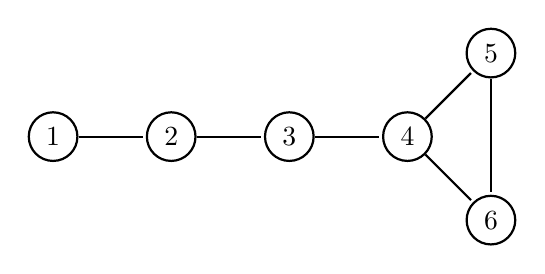
\begin{tikzpicture}[-,>=stealth,shorten >=1pt,auto,node distance=1.5cm, thick,main node/.style={scale=0.9,circle,draw,font=\sffamily\normalsize}]

            \node[circle, draw] (1) []{1};
            \node[circle, draw] (2) [right of = 1]{2};
            \node[circle, draw] (3) [right of = 2]{3};
            \node[circle, draw] (4) [right of = 3]{4};
            \node[circle, draw] (5) [above right of = 4]{5};
            \node[circle, draw] (6) [below right of = 4]{6};

            % \path[every node/.style={font=\sffamily\small}]

            \draw[-] (1) to (2);
            \draw[-] (2) to (3);
            \draw[-] (3) to (4);
            \draw[-] (4) to (5);
            \draw[-] (4) to (6);
            \draw[-] (5) to (6);

            ;
        \end{tikzpicture}
        % \caption{Given the set of red vertices $S$, the green edges represent $\mathrm{cut}(S)$.}
    \end{figure}

    In this graph, our improved version of Charikar would still need $n$ iterations to remove all the vertices --- in the figure, the node labeled with the number $i$ is the only node present in $A_i$ at the $i$-th iteration of the algorithm. Can we do better?

    Consider the proof of \cref{charikar approx}; the second claim of the theorem uses the fact that the vertex $v_i$ has minimum degree in $G[S_{i - 1}]$. However, note that the only reason why we need this fact is to bound $$\deg_{G[S_{i - 1}]}(v_i) \le \avg_{v \in S_{i - 1}}{\deg_{G[S_{i - 1}]}(v_i)}$$ Hence, we may try to use the \tit{average degree} instead of the \tit{minimum degree}, in the definition of $A_i$.

    Consider a path $P_n$; observe that $\textsc{CharikarImproved}(P_n)$ would require $\ceil{\tfrac{n}{2}}$ iteration to remove all the vertices from the initial graph, because it would remove at most (for the case when $n$ is odd) 2 vertices per iteration --- i.e. the endpoints. What happens if we replace the definition of $A_i$ as follows? $$A_i := \cbk{v \in S_i \mid \deg_{G[S_i]}(v) \le \avg_{u \in S_i}{\deg_{G[S_i]}(u)}}$$ In the case of $P_n$, \textsc{CharikarImproved} would still fail at processing the graph all at once, because the average degree is \tit{less than} 2. Nonetheless, this problem suggests the following approach.

    \begin{framedalgo}{Charikar's algorithm ($\varepsilon$ version)}
        Given an undirected graph $G = (V, E)$, the algorithm returns a $\tfrac{1}{2(1 + \varepsilon)}$-approximation solution of DS on $G$. \\
        \hrule

        \quad
        \begin{algorithmic}[1]
            \Function{$\textsc{Charikar}_\varepsilon$}{$G$}
                \State $S_0 := V(G)$
                \State $i := 0$
                \While{$S_i \neq \varnothing$}
                    \State $\displaystyle A_i := \cbk{v \in S_i \mid \deg_{G[S_i]}(v) \le (1 + \varepsilon)\avg_{u \in S_i}{\deg_{G[S_i]}(u)}}$
                    \State $S_{i + 1} := S_i - A_i$
                \EndWhile
                \State \textbf{return} $\displaystyle S^* \in \argmax_{i \in \N}{\rho(G[S_i])}$
            \EndFunction
        \end{algorithmic}
    \end{framedalgo}

    \begin{framedthm}{}
        Given a graph $G$, and $S := \textsc{Charikar}_\varepsilon$(G), let $S^*$ be an optimal solution to DS on $G$. Then, for all $\varepsilon > 0$ it holds that $\abs S \ge \tfrac{1}{2(1 + \varepsilon)} \abs{S^*}$. Moreover, the algorithm runs in at most $O(\log_{1 + \varepsilon}(n))$ iterations.
    \end{framedthm}

    \begin{proof}
        Consider the optimal solution $S^*$; note that $S^* \neq \varnothing$ because $\rho(G[\varnothing])$ is not defined, and if $\abs{S^*} = 1$, then $\abs{E(G[S^*])} = 0 \implies \rho(G[S^*]) = 0$ meaning that any solution is optimal. Hence, we may assume that $\abs{S^*} \ge 2$.
        
        \claim{
            $\forall v \in S^* \quad \deg_{G[S^*]}(v) \ge \rho(G[S^*])$.
        }{
            Fix a vertex $v \in S^*$. By optimality of $S$, we know that $\rho(G[S^*]) \ge \rho(G[S^* - \{v\}])$. Moreover, note that $$\rho(G[S^* - \{v\}]) = \dfrac{\abs{E(G[S^* - \{v\}])}}{\abs{S^* - \{v\}}} = \dfrac{\abs{E(G[S^*])} - \deg_{G[S^*]}(v)}{\abs{S^*} - 1}$$ Therefore, we have that $$\rho(G[S^*]) \ge \rho(G[S^* - \{v\}]) \iff \dfrac{\abs{E(G[S^*])}}{\abs{S^*}} \ge \dfrac{\abs{E(G[S^*])} - \deg_{G[S^*]}(v)}{\abs{S^*} - 1}$$ and the claim follows by solving the inequality.
        }

        Now, we observe that by construction of the algorithm, at least one node is removed in each iteration, since at least the vertex with minimum degree will be selected, hence $$\min_{v \in S_i}{\deg_{G[S_i]}(v)} \le \avg_{v \in S_i}{\deg_{G[S_i]}(v)} \le (1 + \varepsilon) \avg_{v \in S_i}{\deg_{G[S_i]}(v)}$$ Thus, the alogrithm will eventualy select a verex of $S^*$. Let $i$ be the first iteration such that $A_i \cap S^* \neq \varnothing$. Since $i$ is the smallest iteration with such property, it must hold that $S^* \subseteq S_i$. Hence, for any vertex $v_i \in A_i \cap S^*$ it holds that $$\rho(G[S^*]) \le \deg_{G[S^*]}(v) \le \deg_{G[S_i]}(v) \le (1 + \varepsilon) \avg_{v \in S_i}{\deg_{G[S_i]}(v)} = 2 (1 + \varepsilon) \rho(G[S_{i + 1}])$$ concluding that $$\rho(G[S_i]) \ge \dfrac{1}{2(1 + \varepsilon)}\rho(G[S^*])$$ which means that the solution $S$ returned by the algorithm will be at least as good as a $\tfrac{1}{2 (1 + \varepsilon)}$-approximation $$S \in \argmax_{j \in [n]}{\rho(G[S_j])} \ge \rho(G[S_i]) \ge \dfrac{1}{2(1 + \varepsilon)} \rho(G[S^*])$$

        Now, fix an iteration $k \in [n]$; we observe that
        \begin{equation*}
            \begin{split}
                2 \abs{E(G[S_k])} &= \sum_{v \in S_k}{\deg_{G[S_k]}(v)} \\
                                  &= \sum_{v \in A_k}{\deg_{G[S_k]}(v)} + \sum_{v \in S_k - A_k}{\deg_{G[S_k]}(v)} \\
                                  &\ge \sum_{v \in S_k - A_k}{\deg_{G[S_k]}(v)} \\
                                  &> \sum_{v \in S_k - A_k}{(1 + \varepsilon) \avg_{ u \in S_k}{\deg_{G[S_k]}(v)}} \\
                                  &= (\abs {S_k} - \abs{A_k})(1 + \varepsilon) \avg_{u \in S_k}{\deg_{G[S_k]}(u)} \\
                                  &= \abs{S_{k + 1}}(1 + \varepsilon) \dfrac{2 \abs{E(G[S_k])}}{\abs{S_k}}
            \end{split}
        \end{equation*}
        Thus, we get that $$2 \abs{E(G[S_k])} > \abs{S_{k + 1}} (1 + \varepsilon)\dfrac{2 \abs{E(G[S_k])}}{\abs{S_k}} \implies 1 > \dfrac{\abs{S_{k + 1}}}{S_k}(1 + \varepsilon) \implies \abs{S_{k + 1}} < \dfrac{\abs{S_k}}{1 + \varepsilon}$$

        Finally, let $i^*$ be the last iteration of the algorithm; since $\abs{S_0} = n$ and $i^*$ is reached when $\abs{S_{i^*}} = 1$, we conclude that $$\abs{S^*} < \dfrac{n}{(1 + \varepsilon)^{i^*}} \implies 1 < \dfrac{n}{(1 + \varepsilon)^{i^*}} \implies i^* \le \log_{1 + \varepsilon}{n}$$
    \end{proof}

    \section{Approximation through semidefinite programming}

    In \cref{maxcut} we mentioned that the best known approximation ratio for the Max-Cut problem is around 0.878. We are now ready to discuss this ratio.

    First, let's look at the approaches that we used for the approximation we presented: we provided a $\tfrac{1}{2}$-approximation for Max-Cut that does not even look at the structure of the graph itself, and simply flips coins in order to decide if the corresponding vertex has to be added to the output.

    Now, let us build an IP that models the Max-Cut problem: for each edge $\{i, j\}$ define a variable $y_{ij}$, and for each vertex define a variable $x_v$.

    \begin{figure}[H]
        \centering
        \[\begin{array}{ccl}
            \qquad\qquad\quad
            & \max \; \displaystyle \sum_{ij \in E(G)}{y_{ij}} \\\\
            & y_{ij} \le x_i + x_j & \forall \{i, j\} \in E(G) \\
            & y_{ij} \le 2 - (x_i + x_j) & \forall \{i, j\} \in E(G) \\
            & x_v \in \{0,1\} & \forall u \in V(G) \\
            & y_{ij} \in \{0,1\} & \forall \{i, j\} \in E(G) \\
        \end{array}\]
        \caption{IP for MC.}
    \end{figure}

    We observe that the constraints on $y_{ij}$ ensure that $y_{ij} = 1$ if and only if $x_i \neq x_j$. Moreover, we don't need to force $y_{ij} = 1$ when $i$ is in the set and $j$ is not (or vice versa) because the \tit{maximization} will enforce this in the solution automatically.

    Now, let us consider the LP relaxation of this IP: the optimal solution of such relaxation will always set every single vertex variable $x_v$ to $\tfrac{1}{2}$, and every edge variable $y_{ij}$ to 1. In other words, the optimal solution to the LP relaxation gives \tit{no information}. Indeed, this is exactly the reason why the $\tfrac{1}{2}$-approximation we presented can just flip coints for every vertex without even looking at the structure of the input.

    Then, how good can this relaxation get? Since our algorithm is a $\tfrac{1}{2}$-approximation, we already know that $\mbox{IG}_\mathrm{MC} \le 2$. Moreover, it can be proven that for any $n \in \N$ the gap of $K_n$ is at least $2 - \varepsilon$ for $\varepsilon > 0$, concluding that $\mbox{IG}_{\mathrm{MC}} = 2$.

    Despite many efforts, for a very long time researchers believed that no improvement over this result could be achieved. However, in a groundbreaking paper published in 1995 \textcite{goemans} proved everyone wrong, by completely changing the approach: instead of using an IP, they modeled the Max-Cut problem through a \tbf{Quadratic Program} (QP). The following is an example of a generic QP.

    \begin{figure}[H]
        \centering
        \[\begin{array}{ccl}
            \qquad\qquad\quad
            & \max \; \dfrac{1}{2} x^TQx + c^Tx \\\\
            & Ax \le b \\
            & x \in V \\
        \end{array}\]
        \caption{Standard form of a QP.}
    \end{figure}

    The QP that exactly models the Max-Cut is very similar to the IP we previously discussed, with the exception of edge constraints being \curlyquotes{implicit} in the objective function.

    \begin{figure}[H]
        \centering
        \[\begin{array}{ccl}
            \qquad\qquad\quad
            & \max \; \displaystyle \sum_{ij \in E(G)}{\dfrac{1 - x_i x_j}{2}} \\\\
            & x_v \in \{-1, 1\} & \forall v \in V(G) \\
        \end{array}\]
        \caption{QP for MC.}
    \end{figure}

    In fact, we observe that for any edge $\{i, j\} \in E(G)$ we have that $$\dfrac{1 - x_ix_j}{2} = \soe{ll}{0 & x_i = x_j \\ 1 & x_i \neq x_j}$$

    Nonetheless, solving quadratic programs is also \NPclass-hard. However, the \tit{ingenious} idea of Goemans and Williamson was to \tit{cast} this QP into a \tbf{Semidefinite Prorgam} (SDP).

    \begin{figure}[H]
        \centering
        \[\begin{array}{ccl}
            \qquad\qquad\quad
            & \max \; \displaystyle \sum_{i,j \in [n]}{c_{i, j } \abk{v_i, v_j}} \\\\
            & \max \; \sum\limits_{i, j \in [n]}{a_{i, j , k} \abk{v_i, v_j}} \le b_k & \forall k \in [n] \\
            & v_i \in \R^n & \forall i \in [n]\\
        \end{array}\]
        \caption{Standard form of an SDP.}
    \end{figure}

    Differently from IPs and QPs, SDPs work on \tit{vector variables}, where $\abk{v_i, v_j}$ denotes the dot product between the two vectors. However, SDPs can also be solved in polynomial time --- like LPs --- through an extension of the Ellipsoid method.

    The following is Goemans and Williamson's SDP relaxation for the Max-Cut problem:

    \begin{figure}[H]
        \centering
        \[\begin{array}{ccl}
            \qquad\qquad\quad
            & \max \; \displaystyle \sum_{ij \in E(G)}{\dfrac{1 - \abk{v_i, v_j}}{2}} \\\\
            & \abk{v_i, v_i} = 1 & \forall i \in [n] \\
            & v_i \in \R^n & \forall i \in [n] \\
        \end{array}\]
        \caption{SPD for MC.}
    \end{figure}

    Let $\overline x$ be a feasible solution to the QP. If we map each component $\overline x_i$ with the vector $v_i = [\overline x_i \ 0 \ \cdots \ 0]^T$, we see that $$\abk{v_i, v_j} = \sum_{k \in [n]}{v_{k}(i) \cdot v_k(j)} = \overline x_i \overline x_j$$ Moreover, we observe that  the constraint $\abk{v_i, v_i} = 1$ is always satisfied $$\abk{v_i, v_i} = \sum_{k \in [n]}{v_k(i)^2} = {\overline x_i}^2 = 2$$ This concludes that $$\mathrm{SDP}^*_\mathrm{MC} \ge \mathrm{QP}^*$$

    However, the algorithm proposed by the two authors is \tit{very} surprising.

    \begin{framedalgo}[label={gw algo}]{GW approximation for Max-Cut}
        Given a graph $G$, the algorithm returns a cut of $G$. \\
        \hrule

        \quad
        \begin{algorithmic}[1]
            \Function{GWapprox}{$G$}
                \State $\{v_1, \ldots, v_n\} := \mathrm{SDP}_\mathrm{MC}(G)$
                \State $S_n := \{x \in \R^n \mid \norm{x} = 1\}$ \Comment{$S_n$ is the $n$-dimensional hypersphere of radius 1}
                \State Sample a vector $y$ from $S_n$ UAR
                \State $S := \{i \mid \abk{v_i, y} \ge 0\}$
                \State \tbf{return} $S$
            \EndFunction
        \end{algorithmic}
    \end{framedalgo}

    \begin{framedthm}{}
        Given a graph $G$, let $S^*$ be an optimal solution to MC of $G$; then, if $S = \textsc{GWapprox}(G)$, it holds that $$\Exp \sbk{\abs{\mathrm{cut}(S)}} \ge \alpha_{\mathrm{GW}} \cdot \abs{\mathrm{cut}(S^*)}$$ where $$\alpha_{\mathrm{GW}} = \dfrac{2}{\pi} \min_{x \in (-1, 1)}{\dfrac{\arccos(x)}{\pi}} = 0.878  \ldots$$
    \end{framedthm}

    \begin{proof}
        Omitted.
    \end{proof}

    We observe that the approximation ratio $\alpha_{\mathrm{GW}}$ is actually \tit{tight}. In fact, it can be proven that $\mathrm{IG}_{\mathrm{MC}}^{\mathrm{SDP}} = \alpha_{\mathrm{GW}}$, where the upper bound is given by the graph $C_n$ --- details omitted.

    \begin{framedthm}{}
        $\mathrm{IG}_{\mathrm{MC}}^{\mathrm{SDP}} = \alpha_{\mathrm{GW}}$
    \end{framedthm}

    This concludes that Goemans and Williamson's algorithm is \tit{the best} rounding algorithm that can be achieved through SDPs. Moreover, researchers believe that this approximation is the best that can be achieved \tit{in general} for MC. In particular, the main reasong behind such hypothesis is the \tbf{Unique Games Conjecture}, which will be discussed in the following section.

    \section{The Unique Games Conjecture}

    Before discussing the conjecture itself, consider the following definition.

    \begin{frameddefn}{Unique label cover}
        Let $G$ be a bipartite graph, bipartitioned through $(A, B)$; given a value $k \in \N$, for each edge $e \in E(G)$ let $\func{\pi_e}{[k]}{[k]}$ be a permutation. A \tbf{unique label cover} (ULC) of $G$ is an assignment $\func{\phi}{A \cup B}{[k]}$ defining the set $S_\phi$ of satisfied edges: $$S_\phi := \{ab \in E(G) \mid a \in A, b \in B, \pi_{ab}(\phi(a)) = \phi(b)\}$$
    \end{frameddefn}

    In other words, an edge $ab \in E(G)$ of $G$ is sait to be \tit{satisfied} by $\phi$ if the color $\phi(a)$ gets permuted into the color $\phi(b)$ by the permutation $\pi_{ab}$.

    \centeredimage[In this figure, (a) and (b) are two instances of the UCL problem with 2 colors; (b) is a solution to (a) that satisfies all the edges, while (d) is a solution to (c) with an unsatisfied edge.]{0.8}{../assets/ucl.png}

    Note that UCL instances are \tit{strongly constrainted}, i.e. the color of a vertex uniquely defines the colors of its neighbors, and therefore its entire connected component. Thus, if the input instance admits a valid assignment, such assignment can be found \tit{efficiently} by iterating over all the possible colors of a single node. In particular, this implies that the problem of deciding if a given instance admits a satisfying assignment can be solved in polynomial time.

    The \tbf{value} of a UCL instance is the ratio of the edges that are satisfiable by any assignment. Hence, for satisfiable instances the ratio is 1, and we can find a satisfiying assignment as described. In contrast, determining the value of an unsatisfiable game --- even approximately --- appears to be very hard. This difficulty was formalized by \textcite{khot} in terms of \NPclass-hardness, as follows.

    \begin{framedconj}{Unique Games Conjecture (UGC)}
        It is conjectured that for each $\varepsilon > 0$ there is a value $k_\varepsilon$ for which it is $\NPclass-hard$ to determine if for a UCL instance with $k_\varepsilon$ labels one of the following holds:

        \begin{itemize}
            \item at most an $\varepsilon$-fraction of the edges are satisfied
            \item at least a $(1 - \varepsilon)$-fraction of the edges are satisfied
        \end{itemize}
    \end{framedconj}

    Furthermore, Khot's conjecture has been shown to be linked with \href{https://en.wikipedia.org/wiki/Constraint_satisfaction_problem}{Constraint Satisfaction Problems}, a particular type of optimization problems defined as follows.

    \begin{frameddefn}{Constraint Satisfaction Problem}
        Let $\mathcal P$ be a set of $k$-ary predicates defined on $[q]$, for $q, k \in \N$. An instance of a \tbf{Constraint Satisfaction Problem} (CSP) is a set of variables $X = \{x_1, \ldots, x_n\}$ and a set of constraints $C_1, \ldots, C_m$ such that $C_j = \abk{I_j, P_j}$ where $I_j \subseteq [n]$ and $P_j \in \mathcal P$.

        A constraint $C_j = \abk{I_j, P_j}$ is said to be \tit{satisfied} by an assignment $\func{\alpha}{I_j}{\{0, 1\}}$ if $P_j \smat{x_{i_1} & \ldots & x_{i_k} \\ \alpha(x_{i_1}) & \ldots & \alpha(x_{i_k})}$ evaluates to true.
    \end{frameddefn}

    The goal of a CSP is to find an assignment maximizing the number of satisfied constraints. Many optimization problems can be described in terms of CSP, and in particular the Max-Cut problem --- which we mentioned at the end of the previous section. In fact, MC can be described through a CSP with value $q = 2$, and predicate set $\mathcal P = \{p(a, b)\}$ with arity 2, where $p(a, b) = \mbox{\curlyquotes{$a \neq b$}}$. Then, given a graph $G$, for each node $x \in V(G)$ we define the variable $x_v$, and for each edge $uv \in E(G)$ we define the constraint $p(x_u, x_v)$.
    
    Given a problem that can be described through a CSP $\mathcal C$, let $\alpha(\mathcal C)$ be the best possible approximation ratio for $\mathcal C$, i.e. the minimum ratio such that the problem does not become \NPclass-hard to approximate. The following theorem, proved by \textcite{raghavendra}, shows that the relationship between approximation algorithms, SDPs, and the UGC is as strong as it can be.

    \begin{framedthm}{Raghavendra's theorem}
        For every CSP $\mathcal C$ with values in $[q]$ and arity $k$, the following hold.

        \begin{itemize}
            \item There is an SDP with IG of $\alpha(\mathcal C)$ and a rounding algorithm that is an $\alpha(\mathcal C)$-approximation of $\mathcal C$.
            \item If the UGC is true, it is \NPclass-hard to approximate $\mathcal C$ with a ratio $\alpha(\mathcal C) - \varepsilon$ for any $\varepsilon > 0$.
        \end{itemize}
    \end{framedthm}

    In particular, if the UGC holds true, Raghavendra's theorem implies that the SDP integrality gap for any problem that can be described through a CSP is the best possible approximation ratio that can be achieved. Although many researchers believe in the validity of the conjecture, it remains unproven.

    As a direct corollary of Raghavendra's theorem, we get that the approximation ratios that we previously found for MC and VC are the best possible ones, if the UGC is true.

    \begin{framedcor}{}
        If the UGC is true, then $\mathrm{IG}_{\mathrm{MC}}^{\mathrm{SDP}} = \alpha_\mathrm{MC}$ and $\mathrm{IG}_\mathrm{VC} = \alpha_\mathrm{VC}$.
    \end{framedcor}

    \chapter{Metric geometry}

    TODO \todo{missing introduction}

    First, consider the following definition.

    \begin{frameddefn}{Set spartity}
        Given a graph $G = (V, E)$, and a set $\varnothing \subset S \subseteq V$, the \tbf{sparsity} of $S$ is defined as follows: $$\psi (S) := \dfrac{\abs{\mathrm{cut}(S)}}{\abs{S \times \overline S}} = \dfrac{\abs{\mathrm{cut}(S)}}{\abs S \cdot \abs{\overline S}}$$
    \end{frameddefn}

    As for the case of \tit{graph density}, we require $S \neq \varnothing$, but we will omit this detail in the following sections. Moreover, note that by definition of \tit{cut}, we have that for any $S \subseteq V(G)$ it holds that $$0 \le \abs{\mathrm{cut}(S)} \le \abs {S \times \overline S} = \abs S \cdot \abs{\overline S}$$ since an edge $e$ is in $\mathrm{cut}(S)$ if and only if $\abs {S \cap e} = 1$, hence the cartesian product $S \times \overline S$ represents the edges that have exactly one endpoint in $S$. Therefore, we have that $0 \le \psi(S) \le 1$, and in particular

    \begin{itemize}
        \item $\psi(S) = 0 \implies \abs{\mathrm{cut}(S)} = 0$ which happens if $S$ is \tit{disconnected} from $\overline S$
        \item $\psi(S) = 1 \implies \abs{\mathrm{cut}(S)} = \abs{S \times \overline S}$ which happens if $S$ is \curlyquotes{\tit{fully connected}} to $\overline S$, i.e. every edge of $S$ is connected to every edge of $\overline S$.
    \end{itemize}

    Given this metric, we are interested in finding the subset of vertices of a given graph that \tit{minimizes} its sparsity.

    \begin{frameddefn}{Sparsest Cut problem}
        The \tbf{Sparsest Cut} (SC) problem is defined as follows: given a graph $G = (V, E)$, determine the subset of vertices that minimizes its sparsity. In other words, the problems asks to finde a set $S^*$ in $$S^* \in \argmin_{S \subseteq V}{\psi(S)}$$
    \end{frameddefn}

    In order to reason about SC, we are going to introduce the following type of graphs, invented by \textcite{erdos} in 1959.

    \begin{frameddefn}{Erdős-Rényi random graph}
        Given two values $n \in \N$ and $\mu \in [0, 1]$, the \href{https://en.wikipedia.org/wiki/Erd%C5%91s%E2%80%93R%C3%A9nyi_model}{Erdős-Rényi random graph} $G(n, \mu)$ is a graph that has a fixed vertex set $V(G) = [n]$, and a \tit{probabilistic} edge set $E(G)$ such that $$\forall e \in \binom{V(G)}{2} \quad \Pr[e \in E(G)] = \mu$$
    \end{frameddefn}

    By definition, this model represents an \tit{evenly sparse graph}, because for each $S \subseteq V(G)$ it holds that $$ \mathbb E[\psi(S)] = \dfrac{\mathbb E\sbk{\abs{\mathrm{cut}(S)}}}{\abs S \cdot \abs{\overline S}} = \dfrac{\sum_{ij \in S \times \overline S}{\Pr \sbk{ij \in \mathrm{cut}(S)}}}{\abs S \cdot  \abs{\overline S}}= \dfrac{\mu \cdot \abs S \cdot \abs{\overline S}}{\abs S \cdot \abs{\overline S}} = \mu$$

    The Maximum Cut problem --- which we discussed in \cref{maxcut} --- can be reduced to SC, implying that the latter is \NPclass-hard as well. Nevertheless, the problem can be approximated through the \tbf{Leighton-Rao algorithm} \cite{leightonrao}, which relies on LP relaxation and a series of reduction steps. In particular, its integrality gap is bounded using \tit{geometric arguments}, therefore in the following sections we will focus on \tbf{metric geometry} in order to establish this result.

    \section{Metrics}

    \subsection{Cut metrics}

    A \tbf{metric} (or \tit{distance function}) provides a way to quantify how far apart objects are within a given space, formalizing the concept of \tit{distance}. In particular, in geometry we have the following definition.

    \begin{frameddefn}{Metric}
        Given a set $S$, a \tbf{metric} on $S$ is a function $\func{d}{S \times S}{\R}$ that satisfies

        \begin{enumerate}
            \item \tit{non-negativity}: $\forall x, y \in S \quad d(x,y) \ge 0$
            \item \tit{symmetry}: $\forall x, y \in S \quad d(x, y) = d(y, x)$
            \item \tit{self-distance}: $\forall x \in S \quad d(x, x) = 0$
            \item \tit{triangle inequality}: $\forall x, y, z \in S \quad d(x,y) \le d(x,z) + d(z, y)$
        \end{enumerate}
    \end{frameddefn}

    The typical example of metric is the \href{https://en.wikipedia.org/wiki/Euclidean_distance}{Euclidean distance}, which defines $d$ as follows $$d(x, y) := \norm{x - y}$$ In particular, for our discussion we are interested in \tit{cut metrics}, defined as follows.

    \begin{frameddefn}{Elementary cut metric}
        Given a graph $G = (V, E)$, and a set $T \subseteq V$, the \tbf{elementary cut metric of $T$} is a function $\func{d_T}{V \times V}{\R}$ such that $$d_T(x, y) := \soe{ll}{1 & \abs{T \cap \{x, y\}} = 1 \\ 0 & \mathrm{otherwise}}$$
    \end{frameddefn}

    In other words, for a given set of vertices $T$, the elementary cut metric $d_T(x, y)$ is equal to 1 if and only if the edge $xy$ is in $\mathrm{cut}(T)$.

    \begin{framedprop}{}
        Any elementary cut metric is a metric.
    \end{framedprop}

    \begin{proof}
        Given a graph $G$, and a susbset $T \subseteq V(G)$, consider the elementary cut metric $d_T$; we observe that, by definition

        \begin{itemize}
            \item \tit{non-negativity} is satisfied, because $$\forall x, y \in V(G) \quad d_T(x, y) = 0 \lor d_T(x, y) = 1 \implies d_T(x, y) \ge 0$$
            \item \tit{symmetry} is satisfied, because $$\forall x, y \in V(G) \quad \abs{T \cap \{x, y\}} = \abs{T \cap \{y, x\}} \implies d_T(x, y) = d_T(y, x)$$
            \item \tit{self-distance} is satisfied, because $$\forall x \in V(G) \quad \nexists \{x, x\} \in E(G) \implies d_T(x, x) =0$$
        \end{itemize}
        
        hence, we just need to prove that the \tit{triangle inequality} is also satisfied by $d_T$. Therefore, fix three vertices $x, y, z \in V(G)$; we have three cases:

        \begin{itemize}
            \item if $x, y, z \in T$ then $$0 = d_T(x, y) \le d_T(x, z) + d_T(z, y) = 0 + 0 = 0$$
            \item if $x, y, z \notin T$ then $$0 = d_T(x, y) \le d_T(x, z) + d_T(z, y) = 0 + 0 = 0$$
            \item if $\exists A \in \{T, \overline T\}$ such that \tit{exactly one} of $x, y, z$ lies in $A$, we have three sub-cases:
                \begin{itemize}
                    \item if $x \in A$ then $$1 = d_T(x, y) \le d_T(x, z) + d_T(z, y) = 1 + 0 = 1$$
                    \item if $y \in A$ then $$1 = d_T(x, y) \le d_T(x, z) + d_T(z, y) = 0 + 1 = 1$$
                    \item if $z \in A$ then $$0 = d_T(x, y) \le d_T(x, z) + d_T(z, y) = 1 + 1 = 2$$
                \end{itemize}
        \end{itemize}
    \end{proof}

    We observe that, by definition, for any $T$ it holds that $d_T(x, y) = d_{\overline T}(x, y)$. In fact, if $\{x, y\} \in \mathrm{cut}(T)$ then $\abs{T \cap \{x, y\}} = 1$, meaning that exactly one endpoint of $\{x, y\}$ lies in $T$, which must imply that the other endpont lies in $\overline T$.

    But why are we discussing cut metrics in the first place? We are going to show that the concept of elementary cut metric is \tit{deeply} related to the concept of \tit{sparsity} previously introduced. First, consider the following definition.

    \begin{frameddefn}{Cut-ratio}
        Given a graph $G$, and a subset $T \subseteq V(G)$, the \tbf{cut-ratio} induced by the elementary cut metric $d_T$ is defined as $$\phi(d_T) := \dfrac{\sum_{xy \in E(G)}{d_T(x, y)}}{\sum_{xy \in \binom{V(G)}{2}}{d_T(x, y)}}$$
    \end{frameddefn}

    Unsurprisingly, the following proposition shows that the cut-ratio of $d_T$ is precisely the sparsity of $T$.

    \begin{framedprop}[label={sparse prop}]{}
        Given a graph $G$, and a subset $T \subseteq V(G)$, it holds that $\phi(d_T) = \psi(T)$.
    \end{framedprop}
    
    \begin{proof}
        We observe that $$\phi(d_T) := \dfrac{\sum_{ij \in E(G)}{d_T(x, y)}}{\sum_{ij \in \binom{V(G)}{2}}{d_T(x, y)}} = \dfrac{\sum_{xy \in E(G)}{\1[x \in T \oplus y \in T]}}{\sum_{xy \in \binom{V(G)}{2}}{\1[x \in T \oplus y \in T]}} = \dfrac{\mathrm{cut}(S)}{\abs S \cdot \abs{\overline S}} = \psi(T)$$
    \end{proof}

    We can generalize the concept of elementary cut metric through \tbf{cut metrics}, i.e. linear combinations over a given set of elementary cut metrics, as defined below.

    \begin{frameddefn}{Cut metric}
        Given a graph $G$, a sequence $d_{T_1}, \ldots, d_{T_k}$ of elementary cut metrics on $G$, and $k$ positive real values $\lambda_1, \ldots, \lambda_k > 0$, a \tbf{cut metric} is a function defined as follows $$\funcmap{d}{V(G) \times V(G)}{\R}{(x, y)}{\sum_{i \in [k]}{\lambda_i d_{T_i}(x, y)}}$$
    \end{frameddefn}

    As for elementary cut metrics, it can be easily proven that cut metrics are indeed metrics --- we will omit the proof. Moreover, the following proposition shows that the cut-ratio of a cut metric $d$ is lower bounded by the smallest cut-ratio among the elementary cut metrics that define $d$ itself.

    \begin{framedprop}[label={cut metric prop}]{}
        Given a graph $G$, and a cut metric $d$ defined through $d_{T_1}, \ldots, d_{T_k}$, it holds that $$\phi(d) \ge \min_{j \in [k]}{\phi(d_{T_j})}$$
    \end{framedprop}

    \begin{proof}
        First, consider the following property of sums.

        \claim{
            For any $a_1, \ldots, a_k, b_1, \ldots, b_k > 0$, it holds that $$\dfrac{\sum_{i \in [k]}{a_i}}{\sum_{i \in [k]}{b_i}} \ge \min_{j \in [k]}{\dfrac{a_j}{b_j}}$$
        }{
            We observe that $$\dfrac{\sum_{i \in [k]}{a_i}}{\sum_{i \in [k]}{b_i}} = \dfrac{\sum_{i \in [k]}{\tfrac{b_i}{b_i} \cdot a_i}}{\sum_{i \in [k]}{b_i}} \ge \dfrac{\sum_{i \in [k]}{b_i \cdot \min_{j \in [k]}{\tfrac{a_j}{b_j}}}}{\sum_{i \in [k]}{b_i}} = \min_{j \in [k]}{\dfrac{a_j}{b_j}}$$
        }

        Let $\lambda_1, \ldots, \lambda_k > 0$ be the coefficients that define $d$; then, thanks to the claim, we get
        \begin{equation*}
            \begin{split}
                \phi(d) &= \dfrac{\sum_{xy \in E(G)}{d(x, y)}}{\sum_{xy \in \binom{V(G)}{2}}{d(x, y)}} \\
                        &= \dfrac{\sum_{xy \in E(G)}{\sum_{i \in [k]}{\lambda_i d_{T_i}(x, y)}}}{\sum_{xy \in \binom{V(G)}{2}}{\sum_{i \in [k]}{\lambda_i d_{T_i}(x, y)}}} \\
                        &= \dfrac{\sum_{i \in [k]}{\sum_{xy \in E(G)}{\lambda_i d_{T_i}(x, y)}}}{\sum_{i \in [k]}{\sum_{xy \in \binom{V(G)}{2}}{\lambda_i d_{T_i}(x, y)}}} \\
                        &\ge \min_{j \in [k]}{\dfrac{\sum_{xy \in E(G)}{\lambda_j d_{T_j}(x,y)}}{\sum_{xy \in \binom{V(G)}{2}}{\lambda_j d_{T_j}(x, y)}}} \\
                        &= \min_{j \in [k]}{\dfrac{\sum_{xy \in E(G)}{d_{T_j}(x, y)}}{\sum_{xy \in \binom{V(G)}{2}}{d_{T_j}(x,y)}}} \\
                        &= \min_{j \in [k]}{\phi(d_{T_j})}
            \end{split}
        \end{equation*}
    \end{proof}

    An important consequence of \cref{sparse prop} and \cref{cut metric prop} is the following corollary, which implies that optimizing over \tbf{the sparsest cut} is equivalent to both optimizing over all \tbf{elementary cut metrics} and \tbf{cut metrics} in general.

    \begin{framedcor}{}
        Given a graph $G$, it holds that $$\min_{T \subseteq V(G)}{\psi(T)} = \min_{T \subseteq V(G)}{\phi(d_T)} = \min_{d \ \mathrm{cut \ metric}}{\phi(d)}$$
    \end{framedcor}

    We observe that the last equality derives from the fact that elementary cut metrics are \tit{trivial} cut metrics.

    \subsection{The $\ell_1$ metric}

    Up until this point, we have explored cut metrics in great detail. In the following section, we are going to shift our focus towards other types of metrics, in patricular the $\ell_\mu$ type of metrics, which are defined as shown below.

    \begin{frameddefn}{$\ell_\mu$ metrics}
        Given $\mu \in \R_{\ge 1}$, and a set $S \subseteq \R^d$ for some $d$, the \tbf{$\ell_\mu$ metric} is a function defined as follows $$\ell_\mu(x, y) = \sqrt[\mu]{\sum_{i = 1}^d{\abs{x_i - y_i}^\mu}}$$ We will denote $\ell_\mu(x, y)$ also as $\abs{x - y}_{\ell_\mu}$.
    \end{frameddefn}

    In particular, we are interested in the $\ell_1$ metric. In fact, consider the following definition.

    \begin{frameddefn}{Isometrical embedding}
        Consider two metrics $\func{d_1}{A \times A}{B}$ and $\func{d_2}{X \times X}{Y}$; we say that $d_1$ is \tbf{isometrically embedded} into $d_2$ if there is a function $\func{f}{A}{X}$ such that $$d_1(x, y) = d_2(f(x), f(y))$$
    \end{frameddefn}

    \begin{framedlem}{}
        Any cut metric defined over $k$ cuts is isometrically embedded into $\ell_1$ over $\R^k$.
    \end{framedlem}

    \begin{proof}
        Let $d$ be a cut metric defined over $T_1, \ldots, T_k$, i.e. $d(x, y) = \sum_{i \in [k]}{\lambda_i d_{T_i}(x, y)}$ for some $\lambda_1, \ldots, \lambda_k > 0$. For each $u \in V(G)$, let $\overline{x_u} \in \R^k$ be a vector defined as follows: $$\overline{x_u}(i) := \soe{ll}{\lambda_i & u \in T_i \\ 0 & u \notin T_i}$$ where $\overline{x_u}(i)$ is the $i$-th component of $\overline{x_u}$.

        Now, consider the function $$\funcmap{f}{V(G)}{\R^k}{u}{\overline{x_u}}$$ Now, fix $i \in [k]$, and two vertices $u, v \in V(G)$; we observe that
        
        \begin{itemize}
            \item $\abs{\{u,v\} \cap T_i} = 1 \implies (u \in T_i \land v \notin T_i) \lor (u \notin T_i \land v \in T_i)$; hence, we have that $$u \in T_i \land v \notin T_i \implies \overline{x_u}(i) = \lambda_i \land \overline{x_v}(i)= 0 \implies \abs{\overline{x_u}(i) - \overline{x_v}(i)} = 1$$ and also that $$u \notin T_i \land v \in T_i \implies \overline{x_u}(i) = 0 \land \overline{x_v} (i) = \lambda_i \implies \abs{\overline{x_u}(i) - \overline{x_v}(i)} = 1$$
            \item $\abs{\{u, v\} \cap T_i} = 0 \implies u, v \in T_i \lor u, v \notin T_i$; hence, we have that $$u, v \in T_i \implies \overline{x_u}(i) = \overline{x_v}(i) = \lambda_i \implies \abs{\overline{x_u}(i) - \overline{x_v}(i)} = 0$$ and also that $$u, v \notin T_i \implies \overline{x_u}(i) = \overline{x_v}(i) = 0 \implies \abs{\overline{x_u}(i) - \overline{x_v}(i)} = 0$$
        \end{itemize}

        This means that for any $i \in [k]$ and $u, v \in V(G)$, it holds that $$\1 \sbk{\abs{\{u, v\} \cap T_i} = 1} = \abs{\overline{x_u}(i)- \overline{x_v}(i)}$$ Therefore, we obtain the following
        \begin{equation*}
            \begin{split}
                d(u, v) &= \sum_{i \in [k]}{\lambda_i d_{T_i}(u, v)} \\
                        &= \sum_{i \in [k]}{\lambda_i \cdot \1 \sbk{\abs{\{u, v\} \cap T_i} = 1}} \\
                        &= \sum_{i \in [k]}{\abs{\overline{x_u}(i) - \overline{x_v}(i)}} \\
                        &= \abs{\overline{x_u} - \overline{x_v}}_{\ell_1} \\
            \end{split}
        \end{equation*}
        meaning that $d$ is indeed isometrically embedded into $\ell_1$ over $\R^k$.
    \end{proof}

    \begin{framedlem}[label={metric lemma}]{}
        For any $d$, and any set $X \underset{fin}{\subseteq} \R^d$, the $\ell_1$ metric over $X$ is isometrically embedded into a cut metric defined over $d \cdot(\abs X - 1)$ cuts.
    \end{framedlem}

    \begin{proof}
        We prove the statement for $d =1$, and then extend the proof to all other values of $d$.

        Let $X \underset{fin}{\subseteq} \R^d$, i.e. $X = \{x_1, \ldots, x_n\}$ for some $n \in \N$; moreover, let $\func{\pi}{[n]}{[n]}$ be a permutation of the indices ordering the $n$ elements of $X$ such that they are ordered in \tit{ascending order} $$x_{\pi(1)} \le \ldots \le x_{\pi(n)}$$ For each $j \in [n - 1]$, let $S_j := \{\pi(1), \ldots, \pi(j)\}$; by construction, we have that $$\forall j \in [n - 1] \quad S_1 \subseteq \ldots \subseteq S_j$$ Moreover, for each $j \in [n - 1]$ set $\lambda_j := x_{\pi(j + 1)} - x_{\pi(j)}$; since the indices order the elements of $X$ in ascending order, we know that $\lambda_j \ge 0$ for all $j \in [n - 1]$.

        Define $d$ to be the cut metric over the cuts $S_1, \ldots, S_{n - 1}$ with coefficients $\lambda_1, \ldots, \lambda_{n - 1}$; hence, for each $i$ and $j$ such that $i < j$ we get that
        \begin{equation*}
            \begin{split}
                d(x_{\pi(i)}, x_{\pi(j)}) &= \sum_{t \in [j]}{\lambda_t d_{S_t}(x_{\pi(i)}, x_{\pi(j)})} \\
                                          &= \sum_{t \in [j]}{\lambda_t \cdot \1 \sbk{\abs{\{x_{\pi(i)}, x_{\pi(j)}\} \cap S_t} = 1}} \\
                                          &= \sum_{i \le t < j}{\lambda_t} \\
                                          &= (x_{\pi(j)} - x_{\pi(j - 1)}) + (x_{\pi(j - 1)} - x_{\pi(j - 2)}) + \ldots + (x_{\pi(i + 1)} - x_{\pi(i)}) \\
                                          &= x_{\pi(j)} - x_{\pi(i)} \\
                                          &= \abs{x_{\pi(j)} - x_{\pi(i)}}_{\ell_1}
            \end{split}
        \end{equation*}
        Lastly, since metrics are symmetric, we conclude that $$\forall i,j \quad d(x_{\pi(i)}, x_{\pi(j)}) = \ell_1(x_{\pi(1)}, x_{\pi(j)})$$ which means that for $d=1$ finite $\ell_1$ metrics can be embedded into a cut metric with $\abs X - 1$ cuts. Now, for any dimension $d > 0$, finite $\ell_1$ metrics can be embedded into a cut metric that is the sum of each 1-dimensional embedding, meaning that $\ell_1$ can be embedded into a cut metric with $d \cdot(\abs X - 1)$ cuts.
    \end{proof}

    These two lemmas further improve our optimization equalities: optimizing over a cut metric is equal to optimizing over an \tbf{$\ell_1$ metric}.

    \begin{framedcor}[label={metric cor}]{}
        Given a graph $G$, it holds that $$\min_{T \subseteq V(G)}{\psi(T)} = \min_{T \subseteq V(G)}{\phi(d_T)} = \min_{d \ \mathrm{cut \ metric}}{\phi(d)} = \min_{d \ \ell_1 \ \mathrm{metric}}{\phi(d)}$$
    \end{framedcor}

    \section{Metric relaxations and distortions}

    \subsection{Metric relaxations}

    Consider the following program:

    \begin{figure}[H]
        \centering
        \[\begin{array}{ccl}
            \qquad\qquad\quad
            & \max \; \dfrac{\sum_{ij \in E(G)}{d_{ij}}}{\sum_{ij \in \binom{V(G)}{2}}{d_{ij}}} \\\\
            & \sum\limits_{S \subseteq V(G)}{\lambda_Sd_S(i, j)}  = d_{ij} & \forall ij \in \binom{V(G)}{2} \\
            & \lambda \in \R^{2^n} \\
            & d \in \R^{\abs{\binom{n}{2}}} \\
        \end{array}\]
        \caption{Non-linear program for SC.}
    \end{figure}

    In this \tit{non}-linear program, the variables $d_{ij}$ and $\lambda_S$ --- as their names suggest --- represent the cut values for the optimal cut metric $d^*$ described by the optimal solution, which corresponds to $\phi(d^*)$. Note that the values $d_S(i,j)$ are elementary cut metrics, hence they act as nothing more than a constant coefficient, while we optimize over the values $\lambda_S$ defining the \tit{actual} coefficients of the cut.

    Additionally, the main constraint of the program optimizes over cut metrics, which we proved to be \curlyquotes{isometrically equivalent} to $\ell_1$ metrics in the previous lemmas. Therefore, this program can be viewed as optimizing both over cut metrics and $\ell_1$ metrics. However, the objective function is clearly \tit{non}-linear, hence the program is \tit{non}-linear as well. To fix this, we can normalize the denominator of the objective function since it is shared among all feasible solutions, obtaining the following LP

    \begin{figure}[H]
        \centering
        \[\begin{array}{ccl}
            \qquad\qquad\quad
            & \max \; \displaystyle \sum_{ij \in E(G)}{d_{ij}} \\\\
            & \sum\limits_{S \subseteq V(G)}{\lambda_Sd_S(i, j)}  = d_{ij} & \forall ij \in \binom{V(G)}{2} \\
            & \sum\limits_{ij \in \binom{V(G)}{2}}{d_ij} = 1 \\
            & \lambda \in \R^{2^n} \\
            & d \in \R^{\abs{\binom{n}{2}}} \\
        \end{array}\]
        \caption{LP for SC.}
    \end{figure}

    By construction, the solution to this LP corresponds to the optimal cut metric $d^*$, and the optimal solution to SC is given by the minimal elementary cut describing $d^*$; therefore, this LP could be used to get an \tit{exact} solution to SC. However, we cannot employ this LP because it requires an \tit{exponential} number of variables. To solve this issue, consider the following definition.

    \begin{frameddefn}{Metric distortion}
        Given two metrics $d_1$ and $d_2$ over the same vector space $V$, we say that $d_2$ has a \tbf{distortion} from $d_1$ of at most $\alpha \beta$ if $$\forall x, y \in V \quad \dfrac{d_1(x, y)}{\alpha} \le d_2(x, y) \le \beta d_1(x, y)$$
    \end{frameddefn}

    Metric distortion describes the concept of \tit{similarity} between measures. In 1985 \textcite{bourgain} proved that any finite metric can be isometrically embedded into an $\ell_1$ metric, up to some distortion factor.

    \begin{framedthm}[label={bourgain}]{Bourgain's theorem (computational version)}
        Any metric $d$ on $n$ points can be isometrically embedded in time $n^O(1)$ into an $\ell_1$ metric on $\R^d$, where $d = O(\log^3 n)$ and distortion factor $O(\log n)$.
    \end{framedthm}

    Thanks to this result, \textcite{leightonrao} were able to provide an algorithm that yields an $O(\log n)$-approximation to SC by using the following \tbf{metric LP relaxation}: instead of optimizing over $\ell_1$ metrics, they constructed a relaxation that optimizes over \tit{all} metrics --- introducing the approximation factor of $O(\log n)$, which is precisely the distortion factor.

    \begin{figure}[H]
        \centering
        \[\begin{array}{ccl}
            \qquad\qquad\quad
            & \max \; \displaystyle \sum_{ij \in E(G)}{d_{ij}} \\\\
            & x_{ij} + x_{jk} \ge x_{ik} & \forall i, j ,k \in V(G) \\
            & \sum\limits_{ij \in \binom{V(G)}{2}}{d_{ij}} = 1 \\
            & \lambda \in \R^{2^n} \\
            & d \in \R^{\abs{\binom{V(G)}{2}}} \\
        \end{array}\]
        \caption{Metric LP relaxation for SC.}
    \end{figure}

    \begin{framedalgo}{Leighton-Rao algorithm}
        Given a graph $G$, the algorithm returns a cut of $G$. \\
        \hrule

        \quad
        \begin{algorithmic}[1]
            \Function{LeightonRao}{$G$}
                \State $d := \mathrm{LP}_\mathrm{metric}(G)$
                \State $d' := \textsc{to-}\ell_1\textsc{-metric}(d)$ \Comment{apply \cref{bourgain}}
                \State $d'' := \textsc{to-cut-metric}(d')$ \Comment{apply \cref{metric lemma}}
                \State Let $T_1, \ldots, T_k$ be the $k$ cuts of $d''$
                \State \tbf{return} $\displaystyle S \in \argmin_{i \in [k]}{\phi(T_i)}$
            \EndFunction
        \end{algorithmic}
    \end{framedalgo}
    
    Thanks to \cref{metric cor} and \cref{bourgain}, we obtain the following result.

    \begin{framedthm}{}
        Given a graph $G$, and an optimal solution $S^*$ to SC on $G$, let $S := \textsc{LeightonRao}(G)$. Then, it holds that $$\psi(S) \le O(\log n) \cdot \psi(S^*)$$
    \end{framedthm}
    
    In recent years \textcite{arora} were able to improve the approximation ratio up to $O(\sqrt{\log n})$ through the following SDP.

    \begin{figure}[H]
        \centering
        \[\begin{array}{ccl}
            \qquad\qquad\quad
            & \max \; \displaystyle \sum_{ij \in E(G)}{\abk{x_i,x_i} - 2 \abk{x_i,x_j} + \abk{x_j,x_j}} \\\\
            & \abk{x_i, x_j} - \abk{x_j, x_j} + \abk{x_j, x_k} \le \abk{x_i, x_k} & \forall i, j ,k \in V(G) \\
            & \sum\limits_{ij \in \binom{V(G)}{2}}{\abk{x_i,x_i} - 2 \abk{x_i,x_j} + \abk{x_j,x_j}} = 1 \\
            & \lambda \in \R^{2^n} \\
            & d \in \R^{\abs{\binom{V(G)}{2}}} \\
        \end{array}\]
        \caption{$\ell_2^2$ metric SDP relaxation for SC.}
    \end{figure}

    The idea is similar to that of the Leighton-Rao algorithm: instead of relaxing to every metric, they relax the problem to \tbf{squared $\ell_2$ metrics}. In particular, they observed that
    \begin{equation*}
        \begin{split}
            \ell_2^2(x, y) &= \sum_{i \in [n]}{\abs{x_i - y_i}^2} \\
                           &= \sum_{i \in [n]}{\rbk{x_i^2 - 2x_iy_i + y_i^2}} \\
                           &= \sum_{i \in [n]}{x_i^2 - 2\sum_{i \in [n]}{x_iy_i} + \sum_{i \in [n]}{y_i^2}} \\
                           &= \abk{x,x} - 2 \abk{x,y} + \abk{y,y}
        \end{split}
    \end{equation*}
    Note that $\ell_2^2$ does not always respect the \tit{triangle inequality}. For instance, in $\R$ we have that $\ell_2^2(-1, 0) = \ell_2(0, 1) = 1$, but $\ell_2^2(-1, 1) = 4 > 1$. In fact, the triangle inequality is forced by the second constraint of the SDP itself, in fact: $$\ell_2^2(x, z) + \ell_2^2(z, y) \le \ell_2^2(x, y) \implies$$ $$(\abk{x_i, x_i} - 2\abk{x_i, x_j} + \abk{x_j, x_j}) + (\abk{x_j, x_j} - 2\abk{x_j , x_k} + \abk{x_k, x_k}) \ge \abk{x_i, x_i} - 2 \abk{x_i, x_k} + \abk{x_k, x_k}$$ $$\implies -2 \abk{x_i, x_j} + 2\abk{x_j , x_j} - 2 \abk{x_j , x_k } \ge -2 \abk{x_i , x_k}$$ $$\abk{x_i, x_j} - \abk{x_j , x_j} + \abk{x_j , x_k} \le \abk{x_i, x_k}$$

    \begin{framedprop}{}
        Any $\ell_2^2$ metric on $n$ points can be isometrically embedded in time $n^O(1)$ into an $\ell_1$ metric on $\R^d$ with distortion factor $O(\sqrt{\log n})$.
    \end{framedprop}

    \begin{proof}
        Omitted.
    \end{proof}

    This $O(\sqrt{\log n})$ is the current best known approximation for SC. Moreover, SC cannot be expressed in terms of CSP --- recall that the above SDP is a \tit{relaxation} for the minimal $\ell_2^2$ problem. Furthermore, even if this approximation ratio is believed to be the best possible one, the UGC only implies that there are no constant factor approximations for SC, meaning that the non-constant ratio could be proved to be lower.

    \subsection{Shortest path metric}

    Metric distortion has showed to be a useful tool for various approximation algorithms. However, in some instances there is a \tit{lower bound} on the distortion required in order to embed a metric into another. For instance, consider the following metric.

    \begin{frameddefn}{Shortest path metric}
        Given a graph $G$, the \tbf{shortest path metric} is a function $\func{d}{V(G) \times V(G)}{\R}$ defined as follows

        $$d_G(x, y) = \abs{\{e \in E(P) \mid P \ \mathrm{shortest} \ u \to v \ \mathrm{path}\}}$$
    \end{frameddefn}

    It can be easily proven that this is indeed a metric --- we will omit the proof.

    We are going to show that the shortest path metric cannot be embedded into $\ell_2$ over $\R^d$ without distortion. In particular, we will show the case for the cycle graph $C_4$. Consider the embedding $\func{f}{V(C_4)}{\R^2}$ such that $$f(1) = \rbk{-\dfrac{1}{2}; \dfrac{1}{2}} \quad f(2) = \rbk{\dfrac{1}{2}; \dfrac{1}{2}} \quad f(3) =\rbk{\dfrac{1}{2}; -\dfrac{1}{2}} \quad f(4) = \rbk{-\dfrac{1}{2}; -\dfrac{1}{2}}$$ It is easy to see that this embedding is isometrical from $d_{C_4}$ to $\ell_1$, since all distances are preserved. However, for the $\ell_2$ metric the diagonals are \tit{not} isometric, in fact $$2 = d_{C_4}(1, 3) \neq \ell_2(f(1), f(3)) = \ell_2 \rbk{\rbk{-\dfrac{1}{2}; \dfrac{1}{2}},\rbk{\dfrac{1}{2}; -\dfrac{1}{2}}} = \sqrt 2$$ In particular, this embedding induces a distortion factor of at most $\sqrt 2$. Furthermore, thanks to the following lemma we prove that this distortion factor is actually the \tit{best} that we can achieve.

    \begin{framedlem}{Shortest Diagonal lemma}
        For any $y_1, y_2, y_3, y_4 \in \R^4$ it holds that $$\ell_2^2(y_1, y_3) + \ell_2^2(y_2, y_4) \le \ell_2^2(y_1, y_2) + \ell_2^2(y_2, y_3) + \ell_2^2(y_3, y_4) + \ell_2^2(y_4, y_1)$$
    \end{framedlem}

    \begin{proof}
        We will employ a technique called \tit{sum of squares proof}: the idea is to show that one equation made of sums of squares is equivalent to the square of an other equation, implying that the first one must be always non-negative. We observe that finding the second equation to use as \curlyquotes{comparison} is \tit{very} hard.

        We will prove the lemma coordinate-by-coordinate: fix $t \in [d]$, and for each $i \in [4]$ let $z_i := y_i(t)$ be the $t$-th coordinate of $y_i$.

        \claim{
            For all $t \in [d]$ it holds that \centeredeq{0.9}{$(z_1 - z_4) ^2 + (z_2 - z_3) ^2 + (z_3 - z_4) ^2 + (z_4 - z_1) ^ 2 - (z_1 - z_3) ^2 - (z_2 - z_4)^2 = (z_1 - z_2 + z_3 - z_4)^2$}
        }{
            It can be proven by expanding both the left and right hand side of the quation.
        }

        Because of the claim, we get that $$(z_1 - z_4) ^2 + (z_2 - z_3) ^2 + (z_3 - z_4) ^2 + (z_4 - z_1) ^ 2 - (z_1 - z_3) ^2 - (z_2 - z_4)^2 = (z_1 - z_2 + z_3 - z_4)^2 \ge 0$$ since the LHS is a square. Now, recalling that $\ell_2^2(y_i, y_j) := \sum_{t \in [d]}{(y_t(i) - y_t(j))^2}$, we get that $$\ell_2^2(y_1, y_2) + \ell_2^2(y_2, y_3) + \ell_2^2(y_3, y_4) + \ell_2^2(y_4, y_1) - \ell_2^2(y_1, y_3) - \ell_2^2(y_2, y_4) \ge 0$$
    \end{proof}

    \begin{framedprop}{}
        Any embedding of the shortest path metric $d_{C_4}$ into $\ell_2$ over $\R^d$, for any $d \in \N_{\ge 1}$, has a distortion factor of at least $\sqrt 2$.
    \end{framedprop}

    \begin{proof}
        Fix $d \in \N_{\ge 1}$, and consider an embedding $\func{f}{V(C_4)}{\R^d}$. Without loss of generality, we may assume that $f(i) = x_i$ for each $i \in [4]$. Let $M$ be the maximum $\ell_2$ edge length over all the points embedded into $\R^d$, in other words $$M_{\ell_2} := \max(\ell_2(x_1, x_2), \ell_2(x_2, x_3), \ell_2(x_3, x_4), \ell_2(x_4, x_1))$$ and let $m$ be the minimum $\ell_2$ diagonal length over all the points embedded into $\R^d$, in other words $$m_{\ell_2} := \min(\ell_2(x_1, x_3), \ell_2(x_2, x_4))$$ Thanks to the Shortest Diagonal lemma, we have that
        \begin{equation*}
            \begin{split}
                2m_{\ell_2}^2 &\le \ell_2^2(y_1, y_3) + \ell_2^2(y_2, y_4) \\
                     &\le \ell_2^2(y_1, y_2) + \ell_2^2(y_2, y_3) + \ell_2^2(y_3, y_4) + \ell_2^2(y_4, y_1) \\
                     &\le 4M_{\ell_2}^2
            \end{split}
        \end{equation*}
        implying that $2m_{\ell_2}^2 \le 4M_{\ell_2}^2 \iff m_{\ell_2} \le \sqrt 2 M_{\ell_2}$. Now, note that the maximum edge length $M_{C_4}$ w.r.t. $d_{C_4}$ is 1, and the minimum diagonal length $m_{C_4}$ w.r.t. $d_{C_4}$ is 2, which means that $m_{C_4} = 2 M_{C_4}$. Therefore, the embedding must have applied a distortion factor of at least $\sqrt 2$.
    \end{proof}

    \section{Exercises}
    
    \chapter{Submodular optimization}

    \tbf{Submodular optimization} plays a central role in \href{https://en.wikipedia.org/wiki/Discrete_optimization}{discrete optimization}, particularly in algorithmic settings where efficiency and approximation guarantees are critical. Submodular functions model a \tit{diminishing returns} property that arises naturally in many computational problems, such as influence maximization, data summarization, and sensor placement. But before introducing submodular optimization in detail, we will discuss the following problem.

    \begin{frameddefn}{Max Cover problem}
        The \tbf{Max Cover} (MC) problem is defined as follows: given a \tit{universe} (or \tit{ground}) set $\mathcal U = [n]$, a collection of sets $C = \{S_1, \ldots, S_m \}$ such that $S_i \subseteq \mathcal U$, and an integer $k \ge 1$, determine the sub-collection $S \subseteq C$ such that $\abs S = k$ that maximizes $\abs{\bigcup_{S_j \in S}{S_j}}$.
    \end{frameddefn}

    In other words, we are asked to determine the sub-collection of the given $C$ of $k$ sets that covers as many elements of $\mathcal U$ as possible. For instance, given $\mathcal U = [7]$, $S_1 = \{1, 2\}$, $S_2 = \{2, 3\}$, $S_3 = \{3, 4, 5\}$, $S_4 = \{5, 6, 7\}$, and $k = 2$, an optimal solution would be $S = \{S_1, S_3\}$ because $\abs{S_1 \cup S_3} = \abs{\{1, 2, 3, 4, 5\}} = 5$.

    The approximation of MC is \tit{solved}, meaning that the best known approximation ratio of $1 - \tfrac{1}{e}$ has been proven to be tight under \NPclass-hardness. Such approximation ratio can be achieved through the following greedy algorithm.

    \begin{framedalgo}{$\rbk{1 - \frac{1}{e}}$-approximation for MC}
        Given an instance of MC $(\mathcal U, C, k)$, the algorithm returns a $\rbk{1 - \tfrac{1}{e}}$-approximation for the instance. \\
        \hrule

        \quad
        \begin{algorithmic}[1]
            \Function{ApproxMaxCover}{$\mathcal U$, $C$, $k$}
                \State $S := \varnothing$
                \State $T_0 := \varnothing$
                \For{$i \in [k]$}
                    \State $\displaystyle S_i \in \argmax_{S_j \in C - S}{\abs{S_j - T_{i - 1}}}$ \Comment{$S_i$ maximizes the number of \curlyquotes{new} elements}
                    \State $S = S \cup \{S_i\}$
                    \State $T_i = T_{i - 1} \cup S_i$
                \EndFor
                \State \tbf{return} $S$
            \EndFunction
        \end{algorithmic}
    \end{framedalgo}

    \begin{framedthm}[label={mc approx ratio}]{}
        Given an instance $(U, C, k)$ of MC, and an optimal solution $S^*$ to MC on $(\mathcal U, C, k)$, let $S := \textsc{ApproxMaxCover}(\mathcal U, C, k)$. Then, it holds that $$\abs{\bigcup_{S_j \in S}{S_j}} \ge \rbk{1 - \dfrac{1}{e}}\abs{\bigcup_{S_j \in S^*}{S_j}}$$
    \end{framedthm}

    \begin{proof}
        Consider an instance $(\mathcal U, C, k)$ of MC, and an optimal solution $S^*$ to it; moreover, let $\displaystyle X^* := \bigcup_{S_j^* \in S^*}{S_j^*}$ be the set of elements of $\mathcal U$ covered by $S^*$.

        Let $S := \textsc{ApproxMaxCover}(\mathcal U, C, k)$; hence, we have that $T_i = \bigcup_{j = 1}^i{S_j}$. Additionally, let $t_i := \abs{T_i}$ and $\mu_i := \abs{X^*} - t_i$. Hence, we have that
        
        \begin{itemize}
            \item $t_0 = \abs{T_0} = \abs{\varnothing} = 0$
            \item $t_k = \abs{T_k} = \abs{\bigcup_{S_j \in S}{S_j}}$ is the value of $S$
            \item $\mu_0 = \abs{X^*} - t_0 = \abs{X^*} - 0 = \abs{X^*}$ is the value of the optimal solution $S^*$
        \end{itemize}

        Therefore, to prove the approximation ratio of the statement it suffices to show that $t_k \ge \rbk{1 - \tfrac{1}{e}} \mu_0$.

        \claim[Claim 1]{
            $\forall i \in [k] \quad \abs{S_i - T_{i - 1}} \ge \dfrac{\mu_{i - 1}}{k}$
        }{
            Since $S^*$ is an optimal solution that covers $\abs{X^*}$ elements of $\mathcal U$, there must be at least one set $S_j^* \in S^*$ such that $$\abs{S_j^* - T_{i - 1}} \ge \dfrac{\abs{X^*} - \abs{T_{i - 1}}}{k} = \dfrac{\mu_{i - 1}}{k}$$ since otherwise it would be impossible for $S^*$ to cover all of $X^* - T_{i - 1}$.

            Hence, the set $S_i$ selected at the $i$-th iteration is at least \tit{as large as} $S_j^*$, since it is the one maximizing the number of \curlyquotes{new} elements added: $$\abs{S_i - T_{i - 1}} \ge \abs{S^*_j - T_{i - 1}} \ge \dfrac{\mu_{i - 1}}{k}$$
        }

        \claim[Claim 2]{
            $\forall i \in [0, k] \quad \mu_i \le \rbk{1 - \dfrac{1}{k}}^i\abs{X^*}$
        }{
            We will prove the claim by induction on $i$. In particular, if $i = 0$, we have that $$\mu_0 = \abs{X^*} \rbk{1 - \dfrac{1}{k}}^0 \abs{X^*} = 1 \cdot \abs{X^*}$$ hence the base case trivially holds. Then, assuming the inductive hypothesis, we can prove the inductive step as follows
            \begin{equation*}
                \begin{alignedat}{2}
                    \mu_{i + 1} &= \abs{X^*} - t_{i + 1} && \\
                                &= \abs{X^*} - \abs{T_{i + 1}} && \\
                                &= \abs{X^*} - \abs{\bigcup_{j \in [i + 1]}{S_i}} && \\
                                &= \abs{X^*} - \rbk{\abs{\bigcup_{j \in [i]}{S_i}} + \abs{S_{i + 1} - \bigcup_{j \in [i]}{S_i}}} && \\
                                &= \abs{X^*} - (\abs{T_i} + \abs{S_{i + 1} - T_i}) && \\
                                &= \abs{X^*} - \abs{T_i} - \abs{S_{i + 1} - T_i} && \\
                                &\le \mu_i - \dfrac{\mu_i}{k} && \quad \quad (\mbox{by Claim 1}) \\
                                &= \rbk{1 - \dfrac{1}{k}}\mu_i && \\
                                &\le \rbk{1 - \dfrac{1}{k}} \rbk{1 - \dfrac{1}{k}}^i \abs{X^*} && \quad \quad (\mathrm{by \ inductive \ hypothesis \ on} \ \mu_i) \\
                                &= \rbk{1 - \dfrac{1}{k}}^{i + 1}\abs{X^*} && \\
                \end{alignedat}
            \end{equation*}
        }

        By Claim 2, recalling that for any $k \ge 1$ it holds that $\rbk{1 - \tfrac{1}{k}}^k \le e^{-1}$, we get $$\mu_k \le \rbk{1 - \dfrac{1}{k}}^k \abs{X^*} \le \dfrac{1}{e} \abs{X^*}$$ Lastly, since $\mu_k = \abs{X^*} - \abs{T_k}$, we get that $$\abs{X^*} - \abs{T_k} = \mu_k \le \dfrac{1}{e} \abs{X^*} \iff \abs{T_k} \ge \rbk{1 - \dfrac{1}{e}} \abs{X^*} \iff t_k \ge \rbk{1 - \dfrac{1}{e}} \mu_0$$
    \end{proof}

    \section{Submodular functions}

    We are now ready to discuss \tbf{submodular functions}, which play a central role in \tit{submodular optimization} that we introduced at the beginning of the chapter.

    \begin{frameddefn}{Modular functions}
        Given $n \in \N$, let $\func{f}{\powerset([n])}{\R}$ be a function; given two sets $S, T \subseteq [n]$, we say that $f$ is

        \begin{itemize}
            \item a \tbf{submodular function} if $f(S) + f(T) \ge f(S \cup T) + f(S \cap T)$
            \item a \tbf{modular function} if $f(S) + f(T) = f(S \cup T) + f(S \cap T)$
            \item a \tbf{supermodular function} if $f(S) + f(T) \le f(S \cup T) + f(S \cap T)$
        \end{itemize}
    \end{frameddefn}

    For instance, for any $n \in \N$ the \tit{cardinality} function, i.e. $f(S) = \abs S$ is modular, because $\forall S, T \subseteq [n] \quad f(S \cup T) = f(S) + f(T) - f(S \cap T)$ by the \href{https://en.wikipedia.org/wiki/Inclusion%E2%80%93exclusion_principle}{inclusion-exclusion principle}. We observe that submodular and supermodular functions are modular, therefore any property that holds for modular functions is true for the other two types as well.
    
    The main property of modular functions is the property to \curlyquotes{know the full description of the function} through at most $n + 1$ values. For example, if $f$ is modular, then the value of $f(\{1, 2, 3\})$ can be computed through $f(\varnothing)$, $f(\{1\})$, $f(\{2\})$ and $f(\{3\})$ as follows $$f(\{1, 2, 3\}) = f(\{1, 2\}) + f(\{3\})- f(\varnothing) = (f(\{1\}) + f(\{2\}) - f(\varnothing)) + f(\{3\}) - f(\varnothing)$$

    \begin{framedprop}{}
        For any $n \in \N$, the function $\func{f}{\powerset([n])}{\R}$ is modular if and only if there exist $z, w_1, \ldots, w_n$ such that for all $S \subseteq [n]$ it holds that $f(S) = z + \sum_{i \in S}{w_i}$.
    \end{framedprop}

    \begin{proof}
        Let $f$ be a modular function defined on $n \in \N$, and fix a set $S \subseteq [n]$; in particular, let $S = \{1, \ldots, k\}$. By modularity of $f$, we have that
        \begin{equation*}
            \begin{split}
                f(S) &= f(\{1, \ldots, k\}) \\
                     &= f(\{2, \ldots, k\}) + f(\{1\}) - f(\varnothing) \\
                     &= (f(\{3, \ldots, k\}) + f(\{2\}) - f(\varnothing)) + f(\{1\}) - f(\varnothing) \\
                     &= f(\{k\}) + \sum_{i \in S - \{k\}}{(f(\{i\}) - f(\varnothing))} \\
                     &= f(\varnothing) + \sum_{i \in S}{f(\{i\}) - f(\varnothing)} \\
                     &= z + \sum_{i \in S}{w_i}
            \end{split}
        \end{equation*}
        where $z := f(\varnothing)$ and $w_i := f(\{i\}) - f(\varnothing)$ for all $i \in S$.

        Vice versa, suppose that there are values $z', w_1', \ldots, w_n'$ such that for all $S \subseteq [n]$ it holds that $f(S) = z' + \sum_{i \in S}{w_i'}$. Fix two sets $S, T \subseteq [n]$; then, we have that
        \begin{equation*}
            \begin{split}
                f(S) + f(T) &= \rbk{z' + \sum_{i \in S}{w_i'}} + \rbk{z' + \sum_{i \in T}{w_i'}} \\
                            &= \rbk{z' + \sum_{i \in S \cap T}{w_i'} + \sum_{i \in S - T}{w_i'}} + \rbk{z' + \sum_{i \in S \cap T}{w_i'} + \sum_{i \in T - S}{w_i'}} \\
                            &= \rbk{z' + \sum_{i \in S \cap T}{w_i'}} + \rbk{z' + \sum_{i \in S - T}{w_i'} + \sum_{i \in S \cap T}{w_i'} + \sum_{i \in T - S}{w_i'}} \\
                            &= f(S \cap T) + f(S \cup T)
            \end{split}
        \end{equation*}
        hence $f$ is modular.
    \end{proof}

    The importance of submodularity in optimization stems from its inherent \tbf{diminishing returns} property. In economics, diminishing returns describe the phenomenon where the incremental output of a production process decreases as the quantity of a single input increases, while all other inputs are held constant.

    \begin{frameddefn}{Diminishing returns}
        Given $n \in \N$, let $\func{f}{\powerset([n])}{\R}$; given $S \subseteq [n]$ and $x \in [n] - S$, the \tbf{return} of $x$ on $S$ for $f$ is defined as $$\Delta_f(x \mid S) = f(S \cup \{x\}) - f(S)$$ We say that $f$ has \tbf{diminishing returns} when it holds that $$\forall A \subseteq B \subseteq [n], x \in [n] - B \quad \Delta_f(x \mid A) \ge \Delta_f(x \mid B)$$
    \end{frameddefn}

    \begin{framedthm}[label={submodular returns}]{}
        For any $n \in \N$, the function $\func{f}{\powerset([n])}{\R}$ is submodular if and only if it has diminishing returns.
    \end{framedthm}

    \proofiff{
        Let $\func{f}{\powerset([n])}{\R}$ be a submodular function for some $n \in \N$, and fix $A \subseteq B \subseteq [n]$ and $x \in [n] - B$; by submodularity of $f$, we have that $$f(A \cup \{x\}) + f(B) \ge f(A \cup \{x\} \cup B) + f((A \cup \{x\}) \cap B)$$ Now, since $A \subseteq B$, and $x \notin B$, we have that $$f(A \cup \{x\}) + f(B) \ge f(B \cup \{x\}) + f(A)$$ Lastly, rearranging the terms, we get that $$\Delta_f(x \mid A) := f(A \cup \{x\}) - f(A) \ge f(B \cup \{x\}) - f(B) =: \Delta_f(x \mid B)$$
    }{
        Proved in \cref{submod ex}.
    }

    Why did we present the Max Cover problem at the beginning of the chapter? MC is a \tbf{submodular optimization} problem, i.e. the problem can be described in terms of the following function, which we will prove is actually \tit{submodular}.

    \begin{frameddefn}{Covering function}
        Given $t \in \N$, let $\mathcal U = [t]$ be the universe set, and let $C = \{A_1, \ldots, A_n\}$ be a collection of subsets $A_i \subseteq \mathcal U$; the \tbf{covering function} $\func{f}{\powerset([n])}{\R}$ is defined as follows: $$\forall S \subseteq [n] \quad f(S) := \abs{\bigcup_{j \in S}{A_j}}$$
    \end{frameddefn}

    For example, given $t = 4$ and $A_1 = \{1, 2, 4\}$, $A_2 = \{2, 3\}$, $A_3 = \{1, 4\}$ --- hence $n = 3$ and $C = \{A_1, A_2, A_3\}$ --- we have that $$f(\{1, 3\}) = \abs{\bigcup_{j \in \{1, 3\}}{A_j}} = \abs{A_1 \cup A_3} = \abs{\{1, 2, 4\}} = 3$$ and so on. In other words, the set $S$ is used to \tit{index} the sets $A_j \in C$.

    \begin{framedprop}[label={covering proof}]{}
        The covering function is non-negative, monotone increasing and submodular.
    \end{framedprop}

    \begin{proof}
        Given a set $X \subseteq [n]$, note that $$f(X) = \sum_{i \in [t]}{\1\sbk{\exists j \in X \quad i \in A_j}} = \sum_{i \in [t]}{f_i(X)}$$ where for each $i \in [t]$ the subfunction $\func{f_i}{\powerset([n])}{\R}$ is defined precisely as $$f_i(X) := \soe{ll}{1 & \exists j \in X \quad i \in A_j \\ 0 & \mathrm{otherwise}}$$

        \claim{
            For all $i \in [t]$, the subfunction $f_i$ is non-negative, monotone increasing and submodular.
        }{
            Fix $i \in [t]$, and $S, T \subseteq [n]$; by definition, we trivially have that $f_i$ is non-negaitve, therefore $f_i(S) + f_i(T) \ge 0$. Moreover, by definition $f_i$ is also monotone increasing, i.e. $S \subseteq T \implies f_i(S) \le f_i(T)$ --- if $f_i(S) = 0$ then the inequality is always satisfied, and $f_i(S) = 1 \iff \exists j \in S \quad i \in A_j$ but $S \subseteq T \implies j \in T$ hence $f_i(T) = 1$.

            To prove submodularity, we observe that since $S \cap T \subseteq S \cup T$ and $f_i \in \{0, 1\}$, we only have two cases:

            \begin{enumerate}
                \item $f_i(S \cup T) = f_i(S \cap T) = 1$. By definition, we have that \centeredeq{0.9}{$f_i(S \cap T) = 1 \iff \exists j \in S \cap T \quad i \in A_j \implies \exists j \in S \land j \in T \quad i \in A_j \iff f_i(S) = f_i(T) = 1$} Hence, we have that $$f_i(S) + f_i(T) = 1 + 1 = f_i(S \cup T) + f_i(S \cap T)$$
                \item $f_i(S \cup T) = 1$ but $f_i(S \cap T) = 0$. By definition \centeredeq{0.9}{$f_i(S \cup T) \implies \exists j \in S \cup T \quad i \in A_j \implies \exists j \in S \lor j \in T \quad i \in A_j \iff f_i(S) + f_i(T) \ge 1$} hence, we have that $$f_i(S) + f_i(T) \ge 1 = f_i(S \cup T) + f_i(S \cap T)$$
            \end{enumerate}
        }

        Lastly, fix $S, T \subseteq [n]$; because of the claim, we know that $f$ is trivially non-negative and monotone increasing. To prove submodularity, thanks to the claim we have that
        \begin{equation*}
            \begin{split}
                f(S) + f(T) &= \sum_{i \in [t]}{f_i(S)} + \sum_{i \in [t]}{f_i(T)} \\
                            &= \sum_{i \in [t]}{\rbk{f_i(S) + f_i(T)}} \\
                            &\ge \sum_{i \in [t]}{\rbk{f_i(S \cup T) + f_i(S \cap T)}} \\
                            &= \sum_{i \in [t]}{f_i(S \cup T)} + \sum_{i \in [t]}{f_i(S \cap T)} \\
                            &= f(S \cup T) + f(S \cap T)
            \end{split}
        \end{equation*}
    \end{proof}

    Since MC is \NPclass-hard, this proposition implies that the problem of maximizing non-negative, monotone increasing, and submodular functions over $k$ elements is \NPclass-hard as well. In fact, the $\rbk{1 - \tfrac{1}{e}}$-approximation for MC that we previously discussed is a specific instance of a more general algorithm, first presented by \textcite{nwf}, that aims at maximizing a Non-Negative and Monotone Increasing (NN-MI) submodular function.

    \begin{framedalgo}[label={nwf approx}]{NWF approximation}
        Given an NN-MI submodular function $\func{f}{\powerset(X)}{\R}$, and a value $k \in \N$, the algorithm returns a subset $S \subseteq X$. \\
        \hrule

        \quad
        \begin{algorithmic}[1]
            \Function{NWFapprox}{$f$, $k$}
                \State $S_0 := \varnothing$
                \For{$i \in [k]$}
                    \State $\displaystyle x_i \in \argmax_{x \in X - S_i}{f(S_i \cup \{x\})}$
                    \State $S_i := S_{i - 1} \cup \{x_i\}$
                \EndFor
                \State \tbf{return} $S_k$
            \EndFunction
        \end{algorithmic}
    \end{framedalgo}

    \begin{framedthm}[label={nwf approx proof}]{}
        Given an NN-MI submodular function $\func{f}{\powerset(X)}{\R}$, a value $k \in \N$, and an optimal set $\displaystyle S^* \in \argmax_{S \in \binom{X}{k}}{f(S)}$, let $S := \textsc{NWFapprox}(f, k)$. Then, it holds that $$f(S) \ge \rbk{1 - \dfrac{1}{e}}f(S^*)$$
    \end{framedthm}

    \begin{proof}
        The following proof is a generalization of the proof of \cref{mc approx ratio}, in which we proved MC's approximation ratio. Let $S^* := \{x_1^*, \ldots, x_k^*\}$.

        \claim[Claim 1]{
            For any $i \in [k - 1]$ it holds that $f(S^*) \le f(S_i) + k(f(S_{i + 1}) - f(S_i)$.
        }{
            Since $f$ is monotone increasing, we know that $f(S^*) \le f(S_i \cup S^*)$. Through some algebraic manipulation, we get that
            \begin{equation*}
                \begin{split}
                    f(S^*) &\le f(S_i \cup S^*) \\
                           &= f \rbk{S_i \cup \bigcup_{i=1}^k{\{x_i^*\}}} \\
                           &= f \rbk{S_i \cup \bigcup_{i=1}^k{\{x_i^*\}}} + \sum_{j = 0}{k -1}{\rbk{-f\rbk{S_i \cup \bigcup_{i = 0}^k{\{x_i^*\}}}} + f \rbk{S_i \cup \bigcup_{i = 0}^j{\{x_i^*\}}}} \\
                           &= \sum_{j = 0}^k{\rbk{f \rbk{S_i \cup \bigcup_{i = 0}^j{\{x_i^*\}}}} - f \rbk{S_i \cup \bigcup_{i = 0}^{j- 1}{\{x_i^*\}}}} + f(S_i) \\
                           &= \sum_{j = 0}^k{\Delta \rbk{x_j^* \mid S_i \cup \bigcup_{i = 0}^j {\{x_i^*\}}}} + f(S_i)
                \end{split}
            \end{equation*}
            By \cref{submodular returns}, we know that $f$ is submodular if and only if it has diminishing returns, hence
            \begin{equation*}
                \begin{split}
                    f(S^*) &\le f(S_i) + \sum_{j = 0}^k{\Delta_f \rbk{x_j^* \mid S_i \cup \bigcup_{i = 0}^j{\{x_i^*\}}}} \\
                           &\le f(S_i) + \sum_{j = 0}^k{\Delta_f(x_j^* \mid S_i)}
                \end{split}
            \end{equation*}
            Finally, by the greedy choice of the algorithm, we conclude that:
            \begin{equation*}
                \begin{split}
                    f(S^*) &\le f(S_i) + \sum_{j = 0}^k{\Delta_f(x_j^* \mid S_i)} \\
                           &\le f(S_i) + \sum_{j = 0}^k{\Delta_f(x_{i + 1} \mid S_i)} \\
                           &= f(S_i) + k \cdot (f(S_i \cup \{x_i + 1\}) - f(S_i)) \\
                           &= f(S_i) + k \cdot (f(S_{i + 1}) - f(S_i))
                \end{split}
            \end{equation*}
        }

        Now, for each $i \in [k]$ let $\delta_i = f(S^*) - f(S_i)$.

        \claim[Claim 2]{
            For all $i \in [k]$ it holds that $\delta_i \ge (1 - \tfrac{1}{k})^i f(S^*)$.
        }{
            We proceed by induction on $i$. For the base case, $i = 0$ therefore we trivially have that $$\rbk{1 - \dfrac{1}{k}}^0 f(S^*) = f(S^*) = f(S^*) - f(S_0) = \delta_0$$ Now, assume the claim is true for any $m \le i$. By Claim 1, we know that
            \begin{equation*}
                \begin{split}
                    \delta_{i + 1} &= f(S^*) - f(S_{i + 1}) \\
                                   &\le k \cdot (f(S_{i + 1}) - f(S_i)) \\
                                   &= k \cdot (f(S_{i + 1}) - f(S^*) + f(S^*) - f(S_i)) \\
                                   &= k \cdot ( -\delta_{i + 1} + \delta_i)
                \end{split}
            \end{equation*}
            which implies that $\delta_{i + 1} \le (1 - \tfrac{1}{k}) \delta_i$. Therefore, by induction we get that $$\delta_{i + 1} \le \rbk{1  - \dfrac{1}{k}} \delta_i \le \rbk{1 - \dfrac{1}{k}}^{i + 1} f(S^*)$$
        }

        Lastly, recalling that for all $x \in \R_{\ge 0}$ it holds that $(1 - \tfrac{1}{k}) \le e^{-1}$, by Claim 2 we conclude that $$f(S^*) - f(S_k) = \delta_k \le \rbk{1 - \dfrac{1}{k}}^k f(S^*) \le e^{-1}f(S^*)$$ which implies that $$f(S_k) \ge \rbk{1 - \dfrac{1}{e}} f(S^*)$$
    \end{proof}

    \section{Property variations}

    What happens when we \tit{drop} some of the properties of NN-MI submodular functions? For instance, consider the following function.

    \begin{frameddefn}{Cut function}
        Given a graph $G$ such that $V(G) = [n]$, the \tbf{cut function} $c$ is a function defined as follows $$\funcmap{c}{\powerset([n])}{\R}{S}{\abs{\mathrm{cut}(S)}}$$
    \end{frameddefn}

    We observe that this function is trivially non-negative and symmetric, but not monotone increasing: given two nodes $x, y \in V(K_3)$, clearly $\{x\} \subseteq \{x, y\}$ but $c(\{x\}) \ge c(\{x, y\})$. Nonetheless, we can still prove that is is submodular, as described below.

    \begin{framedprop}{}
        The cut function is non-negative, symmetric and submodular.
    \end{framedprop}

    \begin{proof}
        The non-negativity and symmetry of the function trivially hold by definition, hence we are going to prove that it is submodular. Fix two sets $S, T \subseteq [n]$, and define the following 4 sets as follows $$A_S := S - T \quad A_T := T - S \quad A_{S, T} := S \cap T \quad A := [n] - (S \cup T)$$ Now, that $$\mathrm{cut}(S) = \mathrm{cut}(A_S, A_T) \cup \mathrm{cut}(A_S, A) \cup \mathrm{cut}(A_{S, T}, A_T) \cup \mathrm{cut}(A_{S, T}, A)$$ meaning that $$c(S) = \abs{\mathrm{cut}(A_S, A_T)} + \abs{\mathrm{cut}(A_S, A)} + \abs{\mathrm{cut}(A_{S, T}, A_T)} + \abs{\mathrm{cut}(A_{S, T}, A)}$$ Similarly, we get that
        \begin{equation*}
            \begin{split}
                c(T) &= \abs{\mathrm{cut}(A_T, A_S)} + \abs{\mathrm{cut}(A_T, A)} + \abs{\mathrm{cut}(A_{S, T}, A_S)} + \abs{\mathrm{cut}(A_{S, T}, A)} \\
                c(S \cup T) &= \abs{\mathrm{cut}(A_S, A)} + \abs{\mathrm{cut}(A_T, A)} + \abs{\mathrm{cut}(A_{S, T}, A)} \\
                c(S \cap T) &= \abs{\mathrm{cut}(A_{S, T}, A_S)} + \abs{\mathrm{cut}(A_{S, T}, A_T)} + \abs{\mathrm{cut}(A_{S, T}, A)}
            \end{split}
        \end{equation*}
        meaning that $$c(S) + c(T) = c(S \cup T) + c(S \cap T) + 2 \abs{\mathrm{cut}(A_S, A_T)} \ge c(S \cup T) + c(S \cap T)$$ implying that $c$ is indeed submodular.
    \end{proof}

    \textcite{fmv} proved that the $\tfrac{1}{2}$-approximation that we discussed in \cref{max cut alg} can be generalized to \tit{any} function that satisfies the same properties of the cut function. Moreover, even though the Max Cut problem has a better approximation ratio given by \cref{gw algo}, for generic functions this bound is actually tight.

    \begin{framedlem}{}
        Given $n \in \N$, if $\func{g}{\powerset([n])}{\R}$ is submodular, it holds that $$\forall S \subseteq [n] \quad \avg_{T \subseteq S}{g(T)} \ge \dfrac{g(\varnothing) + g(S)}{2}$$
    \end{framedlem}

    \begin{proof}
        We proceed by strong induction on $\abs S$. For the base case, if $\abs S = 0$ then $S = \varnothing$, therefore $$g(\varnothing) = \avg_{T \subseteq \varnothing}{g(T)} \ge \dfrac{g(\varnothing) + g(\varnothing)}{2} = g(\varnothing)$$ Now, assume that the statement holds for $\abs S \le i$, and consider $\abs S = i + 1$. Fix $x \in S$, and let $S' := S - \{x\}$ --- in particular $\abs{S'} = i$. Hence, we get that

        \begin{equation*}
            \begin{alignedat}{2}
                \sum_{T \subseteq S}{g(T)} &= \sum_{T' \subseteq S'}{g(T')} + \sum_{T' \subseteq S'}{g(T' \cup \{x\})} && \\
                                           &= \sum_{T' \subseteq S'}{g(T')} + \sum_{T' \subseteq S'}{g(T' \cup \{x\})} + \sum_{T' \subseteq S'}{g(T')} - \sum_{T' \subseteq S'}{g(T')} && \\
                                           &= 2\sum_{T' \subseteq S'}{g(T')} + \sum_{T' \subseteq S'}{(g(T' \cup \{x\}) - g(T'))} && \\
                                           &= 2\sum_{T' \subseteq S'}{g(T')} + \sum_{\substack{T \subseteq S : \\ x \in T}}{(g(T) - g(T \cap S'))} && \\
                                           &\ge 2\sum_{T' \subseteq S'}{g(T')} + \sum_{\substack{T \subseteq S : \\ x \in T}}{(g(T \cup S') - g(S'))} && \quad \quad (\mathrm{by \ submodularity \ of} \ g) \\
                                           &= 2\sum_{T' \subseteq S'}{g(T')} + \sum_{\substack{T \subseteq S : \\ x \in T}}{(g(S) - g(S'))} && \quad \quad (x \in T \implies T \cup S' = S) \\
                                           &= 2\sum_{T' \subseteq S'}{g(T')} + 2^i(g(S) - g(S')) && \quad \quad \rbk{\abs{\{T \subseteq S \mid x \in T\}} = 2^i} \\
            \end{alignedat}
        \end{equation*}
        Now, multiplying both sides of the inequality by $2^{- \abs S}$, we get that $$\avg_{T \subseteq S}{g(T)} = 2^{- \abs S}\sum_{T \subseteq S}{g(T)} \ge 2 ^{1 - \abs S}\sum_{T' \subseteq S'}{g(T')} + 2^{i - \abs S}(g(S) - g(S'))$$ and recalling that $\abs S = i + 1$, we have that
        \begin{equation*}
            \begin{alignedat}{2}
                \avg_{T \subseteq S}{g(T)} &\ge 2^{- i}\sum_{T' \subseteq S'}{g(T')} + 2^{-1}(g(S) - g(S')) && \\
                                           &= \avg_{T' \subseteq S'}{g(T')} + \dfrac{g(S) - g(S')}{2} && \\
                                           &\ge \dfrac{g(\varnothing) + g(S')}{2} + \dfrac{g(S) - g(S')}{2} && \quad \quad (\mathrm{by \ the \ strong \ inductive \ hypothesis}) \\
                                           &= \dfrac{g(\varnothing) + g(S)}{2}
            \end{alignedat}
        \end{equation*}
    \end{proof}

    \begin{framedlem}{}
        Given $n \in \N$, if $\func{g}{\powerset([n])}{\R}$ is submodular, it holds that $$\forall S_1, S_2 \subseteq [n] \quad \avg_{T_1 \subseteq S_1}{\avg_{T_2 \subseteq S_2}{g(T_1 \cup T_2)}} \ge \dfrac{g(\varnothing) + g(S_1) + g(S_2) + g(S_1 \cup S_2)}{4}$$
    \end{framedlem}

    \begin{proof}
        Given $X \subseteq [n]$, for any $T \subseteq [n]$ let $h_X(T) := g(X \cup T)$.

        \claim{
            For any $X \subseteq [n]$, the function $h_X$ is submodular.
        }{
            Fix $A, B \subseteq [n]$; we observe that
            \begin{equation*}
                \begin{split}
                    h_X(A) + h_X(B) &= g(X \cup A) + g(X \cup B) \\
                                    &\ge g(X \cup A \cup B) + g((X \cup A) \cap (X \cup B)) \quad \quad (\mathrm{by \ submodularity \ of} \ g) \\
                                    &= g(X \cup A \cup B) + g(X \cup (A \cap B)) \\
                                    &= h_X(A \cup B) + h_X(A \cap B)
                \end{split}
            \end{equation*}
        }

        Since $h_X$ is submodular, by the previous lemma observe that $$\forall S \subseteq [n] \quad \avg_{T \subseteq S}{h_X(T)} \ge \dfrac{h_X(\varnothing) + h_X(S)}{2} = \dfrac{g(X) + g(X \cup S)}{2}$$ Therefore, for any $S_1, S_2 \subseteq [n]$, we have that
        \begin{equation*}
            \begin{alignedat}{2}
                \avg_{T_1 \subseteq S_1}{\avg_{T_2 \subseteq S_2}{g(T_1 \cup T_2)}} &= \avg_{T_1 \subseteq S_1}{\avg_{T_2 \subseteq S_2}{h_{T_1}(T_2)}} && \\
                                                                                    &\ge \avg_{T_1 \subseteq S_1}{\dfrac{g(T_1) + g(T_1 \cup S_2)}{2}} && \quad \quad (\mathrm{by \ the \ previous \ obs.})\\
                                                                                    &= \dfrac{1}{2}\rbk{\avg_{T_1 \subseteq S_1}{g(T_1)} + \avg_{T_1 \subseteq S_1}{g(T_1 \cup S_2)}} && \\
                                                                                    &= \dfrac{1}{2} \rbk{\avg_{T_1 \subseteq S_1}{g(T_1)} + \avg_{T_1 \subseteq S_1}{h_{S_2}(T_1)}} && \\
                                                                                    &\ge \dfrac{1}{2} \rbk{\dfrac{g(\varnothing) + g(S_1)}{2} + \avg_{T_1 \subseteq S_1}{g_{S_2}(T_1)}} && \quad \quad (\mathrm{by \ the \ previous \ lemma}) \\
                                                                                    &\ge \dfrac{1}{2} \rbk{\dfrac{g(\varnothing) + g(S_1)}{2} + \dfrac{g(S_2) + g(S_2 \cup S_1)}{2}} && \quad \quad (\mathrm{by \ the \ previous \ obs.}) \\
                                                                                    &= \dfrac{g(\varnothing) + g(S_1) + g(S_2) + g(S_1 \cup S_2)}{4} && \\
            \end{alignedat}
        \end{equation*}
    \end{proof}

    \begin{framedthm}{}
        Given $n \in \N$, let $\func{f}{\powerset([n])}{\R}$ be a submodular, non-negative and symmetric function. Given $\displaystyle S^* \in \argmax_{S \subseteq [n]}{f(S)}$, if $R$ is chosen from $[n]$ uniformly at random (UAR), it holds that $$\Exp \sbk{f(R)} \ge \dfrac{1}{2}f(S^*)$$
    \end{framedthm}
    
    \begin{proof}
        If we apply the previous lemma on $S^*$ and $[n] - S^*$, we get that
        \begin{equation*}
            \begin{split}
                \dfrac{f(\varnothing) + f(S^*) + f([n] - S^*) + f([n])}{4} &\le \avg_{T_1 \subseteq S^*}{\avg_{T_2 \subseteq [n] - S^*}{f(T_1 \cup T_2)}} \\
                                                                           &= 2^{- \abs{S^*}} \cdot 2^{- n + \abs{S^*}} \cdot \sum_{T_1 \subseteq S^*}{\sum_{T_2 \subseteq [n] - S^*}{f(T_1 \cup T_2)}} \\
                                                                           &= 2^{-n} \sum_{T_1 \subseteq S^*}{\sum_{T_2 \subseteq [n] - S^*}{f(T_1 \cup T_2)}} \\
                                                                           &= 2^ {-n} \sum_{T \subseteq S^* \cup ([n] - S^*)}{f(T)} \quad \quad (S^* \cap ([n] - S^*) = \varnothing) \\
                                                                           &= 2^{-n} \sum_{T \subseteq [n]}{f(T)} \\
                                                                           &= \avg_{T \subseteq [n]}{f(T)} \\
                                                                           &= \Exp [f(R)]
            \end{split}
        \end{equation*}
        Lastly, observe that
        \begin{equation*}
            \begin{alignedat}{2}
                \Exp[f(R)] &\ge \dfrac{f(\varnothing) + f(S^*) + f([n] - S^*) + f([n])}{4} && \\
                           &\ge \dfrac{f(S^*) + f([n] - S^*)}{4} && \quad \quad (\mbox{by non-negativity of} \ f) \\
                           &= \dfrac{2 f(S^*)}{4} && \quad \quad (\mathrm{by \ symmetry \ of} \ f) \\
                           &= \dfrac{1}{2}f(S^*) && \\
            \end{alignedat}
        \end{equation*}
    \end{proof}

    We observe this proof can be also modified for functions that are non-negative, submodular but \tit{not} symmetric, as shown below.

    \begin{framedthm}{}
        Given $n \in \N$, let $\func{f}{\powerset([n])}{\R}$ be a submodular and non-negative function. Given $\displaystyle S^* \in \argmax_{S \subseteq [n]}{f(S)}$, if $R$ is chosen from $[n]$ UAR, it holds that $$\Exp \sbk{f(R)} \ge \dfrac{1}{2}f(S^*)$$
    \end{framedthm}

    \begin{proof}
         Consider the proof of the previous theorem; by simply replacing the application of the symmetry of $f$ in the last step with another application of the non-negativity, we obtain a $\tfrac{1}{4}$-approximation --- leaving the rest of the proof unchanged.
    \end{proof}

    In conclusion, we showed that
    
    \begin{itemize}
        \item NN-MI submodular functions have a $\rbk{1 - \tfrac{1}{e}}$-approximation
        \item NN-S submodular functions have a $\tfrac{1}{2}$-approximation
        \item NN submodular function have a $\tfrac{1}{4}$-approximation
    \end{itemize}

    Submodularity provides a standard approximation bound to many \NPclass-hard \tit{maximization} problems. Furthermore, these same results can be obtained through \tit{supermodularity} for many \NPclass-hard \tit{minimization} problems.

    \chapter{Online algorithms}

    In previous chapters, we discussed the \tbf{Maximal Matching} problem primarily through its connections to other computational problems. In this section, however, we shift our focus to \tit{matchings} in \tbf{bipartite graphs} --- i.e. the Maximal Bipartite Matching (MBM) problem. These matchings are particularly significant due to their applicability in modeling a wide range of real-world scenarios. A classic example is the \tbf{task assignment problem}, where the goal is to allocate tasks to employees optimally. This can be framed as a \tit{maximum matching} problem in a bipartite graph: one partition represents the \tit{tasks}, the other the \tit{employees}, and edges connect each employee to the tasks they are qualified to perform.

    \begin{figure}[H]
        \centering
        \begin{tikzpicture}[-,>=stealth,shorten >=1pt,auto,node distance=1.5cm, thick,main node/.style={scale=0.9,circle,draw,font=\sffamily\normalsize}]

            \node[circle, draw, fill=Carmine] (1) []{};
            \node[circle, draw, fill=Carmine] (2) [below of = 1]{};
            \node[circle, draw, fill=Carmine] (3) [below of = 2]{};
            \node[circle, draw, fill=Carmine] (4) [below of = 3]{};
            \node[circle, draw, fill=BlueLagoon] (5) [right of = 1]{};
            \node[circle, draw, fill=BlueLagoon] (6) [below of = 5]{};
            \node[circle, draw, fill=BlueLagoon] (7) [below of = 6]{};
            \node[circle, draw, fill=BlueLagoon] (8) [below of = 7]{};

            % \path[every node/.style={font=\sffamily\small}]

            \draw[-] (1) to (5);
            \draw[-] (1) to (6);
            \draw[-] (2) to (7);
            \draw[-] (2) [red] to (8);
            \draw[-] (3) to (6);
            \draw[-] (4) [red] to (5);
            \draw[-] (4) to (8);

            ;
        \end{tikzpicture}
        % \caption{A .}
    \end{figure}

    Consider the matching on the bipartite graph shown in this figure: we observe that it is neither \tit{maximal} nor \tit{maximum}. In fact, we can still add an edge to our matching and obtain a matching of larger cardinality, as shown below:

    \begin{figure}[H]
        \centering
        \begin{tikzpicture}[-,>=stealth,shorten >=1pt,auto,node distance=1.5cm, thick,main node/.style={scale=0.9,circle,draw,font=\sffamily\normalsize}]

            \node[circle, draw, fill=Carmine] (1) []{};
            \node[circle, draw, fill=Carmine] (2) [below of = 1]{};
            \node[circle, draw, fill=Carmine] (3) [below of = 2]{};
            \node[circle, draw, fill=Carmine] (4) [below of = 3]{};
            \node[circle, draw, fill=BlueLagoon] (5) [right of = 1]{};
            \node[circle, draw, fill=BlueLagoon] (6) [below of = 5]{};
            \node[circle, draw, fill=BlueLagoon] (7) [below of = 6]{};
            \node[circle, draw, fill=BlueLagoon] (8) [below of = 7]{};

            % \path[every node/.style={font=\sffamily\small}]

            \draw[-] (1) to (5);
            \draw[-] (1) [red] to (6);
            \draw[-] (2) to (7);
            \draw[-] (2) [red] to (8);
            \draw[-] (3) to (6);
            \draw[-] (4) [red] to (5);
            \draw[-] (4) to (8);

            ;
        \end{tikzpicture}
        % \caption{A matching on a bipartite graph.}
    \end{figure}

    However, this matching is now \tit{maximal}, but not \tit{maximum}. In fact, the following is a matching of the same bipartite graph but that has larger cardinality than the previous one:

    \begin{figure}[H]
        \centering
        \begin{tikzpicture}[-,>=stealth,shorten >=1pt,auto,node distance=1.5cm, thick,main node/.style={scale=0.9,circle,draw,font=\sffamily\normalsize}]

            \node[circle, draw, fill=Carmine] (1) []{};
            \node[circle, draw, fill=Carmine] (2) [below of = 1]{};
            \node[circle, draw, fill=Carmine] (3) [below of = 2]{};
            \node[circle, draw, fill=Carmine] (4) [below of = 3]{};
            \node[circle, draw, fill=BlueLagoon] (5) [right of = 1]{};
            \node[circle, draw, fill=BlueLagoon] (6) [below of = 5]{};
            \node[circle, draw, fill=BlueLagoon] (7) [below of = 6]{};
            \node[circle, draw, fill=BlueLagoon] (8) [below of = 7]{};

            % \path[every node/.style={font=\sffamily\small}]

            \draw[-] (1) [red] to (5);
            \draw[-] (1) to (6);
            \draw[-] (2) [red] to (7);
            \draw[-] (2) to (8);
            \draw[-] (3) [red] to (6);
            \draw[-] (4) to (5);
            \draw[-] (4) [red] to (8);

            ;
        \end{tikzpicture}
        \caption{A matching on a bipartite graph.}
    \end{figure}

    However, let us take a closer look to what differentiates our two matchings: we see that to obtain one from the other we can simply \tit{swap} all the edges of our matching. Moreover, we see that all the edges of the maximal matching actually form a \tit{path}, whose edges alternate between being outside and inside the matching. Furthermore, both the first and the last edge of this path are outside the matching, which must imply that the number of edges \tit{outside} the matching is one more than the number of inside edges.

    In general, given a matching $M$ in a graph $G$, we say that a vertex $v \in V(G)$ is \tbf{free} w.r.t. $M$ if there are no edges $e \in M$ such that $e \cap v \neq \varnothing$. An edge $xy \in E(G)$ is said to be \tit{disjoint} from $M$ if both $x$ and $y$ are free w.r.t. $M$.

    Now, we can formalize the concept that we introduced on this small example through the following definitions.

    \begin{frameddefn}{Alternating path}
        Given a graph $G$, and a matching $M$ on $G$, an \tbf{$M$-alternating path} is a path of $G$ that starts at a free node w.r.t. $M$, and is composed of edges that alternate between $M$ and $E(G) - M$.
    \end{frameddefn}

        \begin{figure}[H]
        \centering
        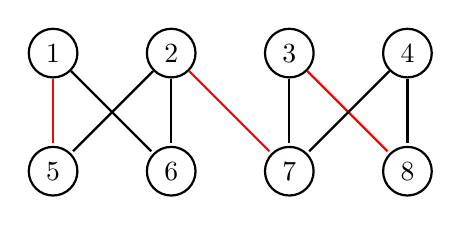
\begin{tikzpicture}[-,>=stealth,shorten >=1pt,auto,node distance=1.5cm, thick,main node/.style={scale=0.9,circle,draw,font=\sffamily\normalsize}]

            \node[circle, draw] (1) []{1};
            \node[circle, draw] (2) [right of = 1]{2};
            \node[circle, draw] (3) [right of = 2]{3};
            \node[circle, draw] (4) [right of = 3]{4};
            \node[circle, draw] (5) [below of = 1]{5};
            \node[circle, draw] (6) [below of = 2]{6};
            \node[circle, draw] (7) [below of = 3]{7};
            \node[circle, draw] (8) [below of = 4]{8};

            \draw[-] (1) [red] to (5);
            \draw[-] (1) to (6);
            \draw[-] (2) to (6);
            \draw[-] (2) to (5);
            \draw[-] (2) [red] to (7);
            \draw[-] (3) to (7);
            \draw[-] (3) [red] to (8);
            \draw[-] (4) to (7);
            \draw[-] (4) to (8);

            ;
        \end{tikzpicture}
        \caption{For instance, if $M$ is the set of \tit{red} edges --- which forms a matching of the graph --- then $6 \ \{6, 2\} \ 2 \ \{2, 7\} \ 7 \ \{7, 3\} \ 3 \ \{3, 8\} \ 8$ is an $M$-alternating path.}
        % \label{}
    \end{figure}

    \begin{frameddefn}{Augmenting path}
        Given a graph $G$, and a matching $M$ on $G$, an \tbf{$M$-augmenting path} is an $M$-alternating path that ends at a free vertex w.r.t. $M$.
    \end{frameddefn}

    For example, if we consider the path $$6 \ \{6, 2\} \ 2 \ \{2, 7\} \ 7 \ \{7, 3\} \ 3 \ \{3, 8\} \ 8 \ \{8, 4 \} \ 4$$ this is actually an $M$-augmenting path of the previous graph. Augmenting paths are very useful because they can be used to \tit{expand} the cardinality of an initial matching. In fact, in the previous graph we can actually define a \tit{larger} matching by \tbf{swapping} the edges of this augmenting path, as shown below

    \begin{figure}[H]
        \centering
        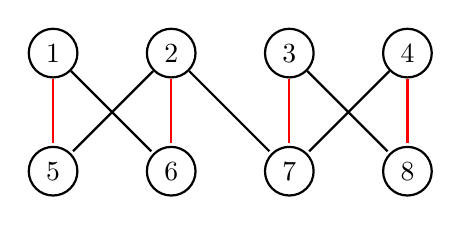
\begin{tikzpicture}[-,>=stealth,shorten >=1pt,auto,node distance=1.5cm, thick,main node/.style={scale=0.9,circle,draw,font=\sffamily\normalsize}]

            \node[circle, draw] (1) []{1};
            \node[circle, draw] (2) [right of = 1]{2};
            \node[circle, draw] (3) [right of = 2]{3};
            \node[circle, draw] (4) [right of = 3]{4};
            \node[circle, draw] (5) [below of = 1]{5};
            \node[circle, draw] (6) [below of = 2]{6};
            \node[circle, draw] (7) [below of = 3]{7};
            \node[circle, draw] (8) [below of = 4]{8};

            \draw[-] (1) [red] to (5);
            \draw[-] (1) to (6);
            \draw[-] (2) [red] to (6);
            \draw[-] (2) to (5);
            \draw[-] (2) to (7);
            \draw[-] (3) [red] to (7);
            \draw[-] (3) to (8);
            \draw[-] (4) to (7);
            \draw[-] (4) [red] to (8);

            ;
        \end{tikzpicture}
        % \caption{For instance, if $M$ is the set of \tit{red} edges --- which forms a matching of the graph --- then $6 \ \{6, 2\} \ 2 \ \{2, 7\} \ 7 \ \{7, 3\} \ 3 \ \{3, 8\} \ 8$ is an $M$-alternating path.}
        % \label{}
    \end{figure}

    This suggests that the presence of augmenting paths in a graph is a \tit{sufficient} condition for a matching \tit{not} to be maximum, but we can actually prove that it is also \tit{necessary}, as stated in the following theorem, proved by \textcite{berge} in 1957.

    \begin{framedthm}[label={aug paths}]{Berge's theorem}
        Given a graph $G$, $M$ is a maximum matching of $G$ if and only if in $G$ there are no $M$-augmenting paths.
    \end{framedthm}

    \proofiff{
        By contrapositive, consider a graph $G$ and a matching $M$ such that there is an $M$-augmenting path $P$ in $G$. Moreover, by way of contradiction assume that $M$ is maximum; however $M \Delta E(P)$ is a larger matching than $M$ --- here, $\Delta$ is the \href{https://en.wikipedia.org/wiki/Symmetric_difference}{symmetric difference}, therefore the operation $M \Delta E(P)$ has the same effect of \tit{swapping} the edges of $P$ between the ones in $M$ and in $E(P) - M$.
    }{
        By contrapositive, consider a graph $G$ and a matching $M$ of $G$ that is not maximum, i.e. there exists a matching $M^*$ of $G$ such that $\abs M < \abs{M^*}$. Consider the subgraph of $G$ that has the vertices of $V(G)$ and the edges described by $M \Delta M^*$; the symmetric difference of these two sets will yield the set of edges that are either in $M$ or in $M^*$, but not in $M \cap M^*$, therefore this subgraph is \tit{not} a multigraph. Moreover, since $M$ and $M^*$ are both matchings, we have that

        \begin{enumerate}[label={(\arabic*)}]
            \item the degrees of the vertices of this subgraph can be either 0, 1 or 2
            \item in each component of the subgraph the edges \tit{must} alternate between $M$ and $M^*$
        \end{enumerate}

        By the observation (1), we have that each component of the subgraph can be either

        \begin{itemize}
            \item a isolated vertex
            \item a cycle
            \item a path
        \end{itemize}

        and by observation (2), we have that all the cycle components must have \tit{even} length, which implies that they have the same number of edges of $M$ and $M^*$. On the other hand, path components may have either even or odd length; in particular, even-length paths must have the same number of edges of $M$ and $M^*$ --- as for cycle components --- while odd-length paths have a different number of edges of $M$ and $M^*$. However, since $\abs M < \abs{M^*}$, there must be at least one path component of this subgraph such that its edges of $M$ are less than the edges of $M^*$, and this is clearly an $M$-augmenting path.
    }

    This theorem has been used to construct many algorithms for finding maximum matchings on bipartite graphs, the easiest one being the following.

    \begin{framedalgo}{Maximum Bipartite Matching}
        Given a bipartite graph $G$, the algorithm returns a maximum matching of $G$. \\
        \hrule

        \quad
        \begin{algorithmic}[1]
            \Function{MaximumBipartiteMatching}{$G$}
                \State $M := \varnothing$
                \While{$\exists P \ M$-augmenting path}
                    \State $M = M \Delta P$
                \EndWhile
            \EndFunction
        \end{algorithmic}
    \end{framedalgo}

    In this algorithm, augmenting paths can be identified using either a DFS or a BFS, resulting in a runtime of $O(mn)$. However, more efficient variants have been developed to reduce this complexity by optimizing the way augmenting paths are found --- most notably, the \href{https://en.wikipedia.org/wiki/Hopcroft%E2%80%93Karp_algorithm}{Hopcroft–Karp algorithm} \cite{hopcroft}. Given a bipartite graph $G$ bipartitioned through $(A, B)$, the key idea is to perform a BFS starting simultaneously from all unmatched vertices in $A$, continuing until at least one free vertex in $B$ is reached; this produces a BFS forest. Then, a DFS is executed over such forest, beginning from the unmatched nodes in $B$, to discover augmenting paths. Each such path allows for alternating the matching along its edges, thereby increasing the overall matching size. The algorithm repeats this process until no more augmenting paths can be found. This approach improves the runtime to $O(m \sqrt n)$, a significant efficiency gain over the basic method.

    % Before ending this section, we are going to discuss the IP for MBM: given a bipartite graph $G = (V, E)$ bipartitioned through $(A, B)$, add a variable $x_{ij}$ for each edge $ij \in E$, and consider the following IP
    %
    % \begin{figure}[H]
    %     \centering
    %     \[\begin{array}{ccl}
    %         \qquad\qquad\quad
    %         & \max \; \displaystyle \sum_{ij \in E} {x_{ij}} \\\\
    %         & \sum\limits_{j \in \mathcal N (i)}{x_{ij}} \le 1 & \forall i \in A \\
    %         & \sum\limits_{i \in \mathcal N (j)}{x_{ij}} \le 1 & \forall j \in B \\
    %         & x_{ij} \in \{0,1\} & \forall ij \in E
    %     \end{array}\]
    %     \caption{IP for MBM.}
    % \end{figure}
    %
    % We observe that this IP indeed models MBM, since
    % 
    % \begin{itemize}
    %     \item for each vertex $i \in A$, the first constraint forces the solution to choose at most one edge incident to $i$
    %     \item for each vertex $j \in B$, the second constraint forces the solution to choose at most one edge incident to $j$
    % \end{itemize}
    %
    % TODO \todo{da finire}

    \section{The online approach}

    An \tbf{online algorithm} processes its input \tit{piece-by-piece} in a sequential manner, without having access to the entire input from the outset. In contrast, a traditional offline algorithm receives \tit{all the input at once} and must then compute a solution. Online algorithms are valuable because they enable solving problems without requiring full knowledge of the data beforehand. The importance of online algorithms has grown significantly with the rise of the Internet and the explosion of big data, where handling massive datasets has made memory management challenging, even for the most advanced supercomputers.

    A practical example of online algorithms is seen in MBM, which is critical for example in online \tbf{advertising services}. Imagine an advertising platform where each user should be matched to \tit{at most one ad per hour}, and each ad can be assigned to \tit{at most one user per hour}. Based on user interests, the platform generates a list of possible ads for each individual. To maximize revenue, it aims to find the \tbf{largest possible matching} between users and ads. This scenario directly corresponds to MBM, where users form one set of the bipartite graph and ads form the other. However, in this context some challenges may arise, for instance

    \begin{itemize}
        \item the sheer volume of users and advertisements makes storing all the data impractical
        \item the set of available users and ads changes continuously, so earlier matches might no longer be optimal
    \end{itemize}

    Online algorithms address both of these issues effectively. Still, because they must make decisions without knowing future inputs, they sometimes produce results that are \tit{not optimal in hindsight}. For instance, suppose that our online algorithm currently knows the following association graph --- in which the \tit{red} nodes indicate the \tbf{ads} and the \tit{blue} ones indicate the \tbf{users}

    \begin{figure}[H]
        \centering
        \begin{tikzpicture}[-,>=stealth,shorten >=1pt,auto,node distance=1.75cm, thick,main node/.style={scale=0.9,circle,draw,font=\sffamily\normalsize}]

            \node[circle, draw, fill=Carmine] (1) []{$A$};
            \node[circle, draw, fill=Carmine] (2) [below of = 1]{$B$};
            \node[circle, draw, fill=BlueLagoon] (3) [right of = 1]{1};

            % \path[every node/.style={font=\sffamily\small}]

            \draw[-] (1) to (3);
            \draw[-] (2) to (3);

            ;
        \end{tikzpicture}
        % \caption{Given the set of red vertices $S$, the green edges represent $\mathrm{cut}(S)$.}
    \end{figure}

    Our algorithm has two options: either match user 1 to ad $A$ or match it to ad $B$. Without loss of generality, assume that user 1 is matched to ad $A$, as shown below

    \begin{figure}[H]
        \centering
        \begin{tikzpicture}[-,>=stealth,shorten >=1pt,auto,node distance=1.75cm, thick,main node/.style={scale=0.9,circle,draw,font=\sffamily\normalsize}]

            \node[circle, draw, fill=Carmine] (1) []{$A$};
            \node[circle, draw, fill=Carmine] (2) [below of = 1]{$B$};
            \node[circle, draw, fill=BlueLagoon] (3) [right of = 1]{1};

            % \path[every node/.style={font=\sffamily\small}]

            \draw[-] (1) [green] to (3);
            \draw[-] (2) to (3);

            ;
        \end{tikzpicture}
        % \caption{Given the set of red vertices $S$, the green edges represent $\mathrm{cut}(S)$.}
    \end{figure}

    Now, suppose that a new user 2 joins our service. After analyzing the preferences of the users, the system determines that only ad $A$ is compatible with user 2, meaning that the latter cannot be assigned any ad since ad $A$ is already matched with user 1.

    \begin{figure}[H]
        \centering
        \begin{tikzpicture}[-,>=stealth,shorten >=1pt,auto,node distance=1.75cm, thick,main node/.style={scale=0.9,circle,draw,font=\sffamily\normalsize}]

            \node[circle, draw, fill=Carmine] (1) []{$A$};
            \node[circle, draw, fill=Carmine] (2) [below of = 1]{$B$};
            \node[circle, draw, fill=BlueLagoon] (3) [right of = 1]{1};
            \node[circle, draw, fill=BlueLagoon] (4) [below of = 3]{2};

            % \path[every node/.style={font=\sffamily\small}]

            \draw[-] (1) [green] to (3);
            \draw[-] (2) to (3);
            \draw[-] (1) to (4);

            ;
        \end{tikzpicture}
        % \caption{Given the set of red vertices $S$, the green edges represent $\mathrm{cut}(S)$.}
    \end{figure}

    However, in hindsight we see that this is \tit{not} the optimal solution: in fact, if our algorithm had matched user 1 to ad $B$, we could've been able to match both users, as shown below

    \begin{figure}[H]
        \centering
        \begin{tikzpicture}[-,>=stealth,shorten >=1pt,auto,node distance=1.75cm, thick,main node/.style={scale=0.9,circle,draw,font=\sffamily\normalsize}]

            \node[circle, draw, fill=Carmine] (1) []{$A$};
            \node[circle, draw, fill=Carmine] (2) [below of = 1]{$B$};
            \node[circle, draw, fill=BlueLagoon] (3) [right of = 1]{1};
            \node[circle, draw, fill=BlueLagoon] (4) [below of = 3]{2};

            % \path[every node/.style={font=\sffamily\small}]

            \draw[-] (1) to (3);
            \draw[-] (2) [green] to (3);
            \draw[-] (1) [green] to (4);

            ;
        \end{tikzpicture}
        \caption{The optimal configuration, \tit{in hindsight}.}
    \end{figure}


    This tendency toward non-optimal solutions is a \tit{defining feature} of online algorithms and is often \tit{unavoidable}. As a result, online algorithms are typically evaluated through \tbf{competitive analysis}, which measures the performance of an online algorithm relative to an optimal offline algorithm. The offline algorithm has the advantage of seeing the entire sequence of requests beforehand, while the online algorithm must respond to an \tit{unpredictable sequence}, making decisions without knowledge of future inputs. Unlike traditional worst-case analysis --- which evaluates an algorithm's behavior only on particularly difficult inputs --- competitive analysis demands strong performance across both easy and hard inputs, where difficulty is determined based on how well the optimal offline algorithm performs.

    To formally assess the competitiveness of online algorithms, researchers employ the \tbf{adversary model}, in which an adversary provides \tit{deliberately challenging inputs} to the algorithm. In the case of deterministic algorithms, the adversary is assumed to have \tit{complete knowledge} of the algorithm's internal workings. Given that the online algorithm cannot anticipate future inputs, this all-knowing adversary can exploit its decisions and lead it into making suboptimal choices.

    In particular, we are going to employ such adversary model to prove the following result.

    \begin{framedthm}[label={mbm det}]{}
        There is no deterministic online algorithm for MBM that can match more than $\tfrac{1}{2}$ of the edges of an optimal solution.
    \end{framedthm}

    \begin{proof}
        We prove the result through an adversarial argument. On the first round, the adversary sends three vertices $a$, $b$, $x$, and two edges $\{a, x\}$ and $\{b, x\}$. The online algorithm has then 3 possible choices for $x$.

        \begin{enumerate}
            \item Match $x$ with $a$. On the next round, the adversary sends a new vertex $y$ and an edge $\{a, y\}$. Since $x$ has been matched to $a$, the new vertex $y$ cannot be matched, meaning that the algorithm returns a solution with a matching having size 1. However, an offline optimal solution would have returned the matching $\{\{b, x\}, \{a, y\}\}$, which has size 2. Therefore, the competitive ratio is $\tfrac{1}{2}$.
            \item Match $x$ with $b$. Similarly to the previous case, on the next round the adversary sends a new vertex $y$ and an edge $\{b, y\}$. Since $x$ has been matched to $b$, the new vertex $y$ cannot be matched, but an offline solution would have returned the matching $\{\{a, x\}, \{b, y\}\}$. Therefore, the competitive ratio is still $\tfrac{1}{2}$.
            \item Leave $x$ unmatched. On the next round, the adversary sends a new vertex $y$ and an edge $\{a, y\}$. Now our algorithm has two options.

                \begin{itemize}
                    \item Match $y$ with $a$; this solution is suboptimal, because an offline algorithm would have matched both $x$ and $y$. Hence, the competitive ratio is again $\tfrac{1}{2}$
                    \item Leave $y$ unmatched; this solution is suboptimal, because an offline algorithm would have matched both $x$ and $y$. Hence, the competitive ratio is 0
                \end{itemize}
        \end{enumerate}

        This concludes that the adversary can always send a set of vertices and edges such that the competitive ratio is at most $\tfrac{1}{2}$.
    \end{proof}

    This result determines an approximation ratio upper bound on \tit{every possible deterministic online algorithm}, concluding that a perfect solution for MBM is \tbf{impossible}. Knowing this, we shift our focus on finding a greedy solution that reaches such maximum approximation ratio. In this case, the best solution is the most straightforward: when a new user arrives, we match it if it can be matched, otherwise we leave it unmatched and proceed with the next round.

    \begin{framedalgo}{The online maximal matching algorithm}
        Given a graph $G$ fed in an online fashion, the algorithm returns a maximal mathing of $G$. \\
        \hrule

        \quad
        \begin{algorithmic}[1]
            \Function{onlineMaximalMatching}{$G$}
                \State $M := \varnothing$
                \While{there is a new user $x$}
                    \State Read $\mathcal N(x)$
                    \State $U(x) := \{v \in \mathcal N(x) \mid \nexists e \in M : v \in e\}$
                    \If{$U(x) \neq \varnothing$}
                        \State Choose $y \in U(x)$
                        \State $M = M \cup \{xy\}$
                    \EndIf
                \EndWhile
                \State \tbf{return} $M$
            \EndFunction
        \end{algorithmic}
    \end{framedalgo}

    The previous theorem, together with the following proposition, imply that this online greedy algorithm is an optimal approximation for MBM.

    \begin{framedprop}{}
        Given a graph $G$, a maximum matching $M^*$ on $G$, and a maximal matching $M$ of $G$, we have that $$\abs M \ge \dfrac{1}{2} \abs{M^*}$$
    \end{framedprop}

    \begin{proof}
        Let $S := \{v \in V(G) \mid \exists e \in M : v \in e\}$ be the set of vertices of $G$ that are matched by edges of $M$. Hence, by definition we have that $\abs S = 2 \abs M$.

        We observe that:

        \begin{itemize}
            \item each node of $S$ is incident to at most one edge of $M^*$, otherwise $M^*$ would not have been a matching
            \item each edge $e \in M^*$ must be incident to at least one node of $S$, since otherwise $M \cup \{e\}$ would be matching that extends $M$, contradicting the fact that it was maximal
        \end{itemize}

        Now, consider a function $\func{f}{M^*}{S}$ such that $f(e) \in S \cap e$: the first observation implies that $f$ is \tit{well-defined}, while the second observation implies that $f$ is \tit{injective}. In particular, this concludes that $$\abs{M^*} \le \abs S = 2 \abs M \iff \abs M \ge \dfrac{1}{2} \abs{M^*}$$
    \end{proof}

    To overcome some of the limitations of \tit{deterministic} online algorithms that we presented, \tbf{randomness} can be introduced into the algorithm's behavior. In randomized online algorithms, the nature of the adversary varies depending on how much information they possess. A commonly studied scenario involves a randomized adversary, where the input sequence is generated according to a \tit{random distribution}. However, even in this setting we can still prove the following result.
    
    \begin{framedthm}{}
        There is no randomized online algorithm for MBM that can expectedly match more than $\tfrac{3}{4}$ of the edges of an optimal solution for graphs chosen from a random distribution.
    \end{framedthm}

    \begin{proof}
        Let $G_1$ be a graph such that $E(G_1) = \{\{a, x\}, \{b, x\}, \{b, y\}\}$, and let $G_2$ be the graph such that $E(G_2) = \{\{a, x\}, \{b, x\}, \{a, y\}\}$. Now, consider a distribution that assigns probability $\tfrac{1}{2}$ to both $G_1$ and $G_2$, and probability 0 to all the other possible graphs.

        On the first round, the adversary sends the edges $\{a, x\}$ and $\{b, x\}$; then, our algorithm will match $x$ to either $a$ or $b$ \todo{what if x unmatched?}, and clearly it will learn nothing about the vertex $y$ whose edges will be sent by the adversary on the next round --- namely, they can send either $\{b, y\}$ or $\{a, y\}$. Through a similar argument used to prove \cref{mbm det}, we see that the probability of $y$ being impossible to match on the next round is $\tfrac{1}{2}$. This implies that $$\Exp[\mbox{number of matched edges}] = TODO$$ TODO \todo{prev eq} However, an offline deterministic algorithm (which is a also randomized algorithm that makes no random choices) can always retun an optimal solution with 2 amtched edges, therefore the expected ratio is $$\dfrac{\tfrac{3}{2}}{2} = \dfrac{3}{4}$$
    \end{proof}

    \subsection{The Market Process algorithm}

    With a similar argument, it can be shown that the bound discussed in the previous section can be improved to $1 - \tfrac{1}{e}$.

    The standard algorithm for the Online Bipartite Matching problem is known as the \tbf{Ranking Algorithm}, originally developed by \textcite{kvv}. The output yielded by this algorithm is guaranteed to be an expected $\rbk{1 - \tfrac{1}{e}}$-approximation, which is tight considering the bound above.

    Over the years, the algorithm has been revised and simplified, while keeping the same approximation ratio. The modern version of this algorithm is known as the \tbf{Market Process Algorithm}, developed by \textcite{eden} --- the name comes from its economics-based interpretation.

    We will refer to the bipartitions of the graph as the pair $(A, U)$, where $A$ is a set of advertisements and $U$ is a set of users.

    \begin{framedalgo}{The Market Process algorithm}
        Given a bipartite graph $G$ with bipartition $(A, U)$, the algorithm returns a matching on $G$. \\
        \hrule

        \quad
        \begin{algorithmic}[1]
            \Function{MarketProcess}{$G$}
                \For{$j \in A$}
                    \State Sample $w_j$ from $[0,1]$ independently and UAR
                    \State $p_j := e^{w_j - 1}$ \Comment{the price of the ad $j$}
                \EndFor
                \State $M := \varnothing$
                    \For{$i \in U$}
                        \State $A' := \{j \in A \mid \nexists i' \in U : \{i', j \} \in M\}$ \Comment{set of unmatched ads}
                        \For{$j \in A'$}
                            \State $v_i(j) := \1[j \in \mathcal N(i)]$ \Comment{the value of ad $j$ for user $i$}
                            \State $u_i(j) := v_i(j) - p_j$ \Comment{the utility of ad $j$ for user $i$}
                        \EndFor
                        \State $u_i(\bot) := 0$ \Comment{the utility of \curlyquotes{not being matched} for user $i$}
                        \If{$A' \cap \mathcal N(i) \neq \varnothing$} \Comment{otherwise $i$ remains unmatched}
                            \State Choose $\displaystyle j^* \in \argmax_{j \in A' \cup \{\bot\}}{u_i(j)}$ \Comment{$j^*$ maximizes the utility for user $i$}
                            \State $M = M \cup \{\{i, j^*\}\}$
                        \EndIf
                    \EndFor
                \State \textbf{return} $M$
            \EndFunction
        \end{algorithmic}
    \end{framedalgo}

    We observe that, on each iteration, for all $j \in A'$ it holds that $u_i(j) \ge 0$ if and only if $j \in \mathcal N (i)$ --- since $v_i(j)$ can only be either 0 or 1 and $$w_j \in [0,1] \implies \tfrac{1}{e} \le p_j := e^{w_j - 1} \le 1$$

    Now, before proving the approximation ratio of the algorithm, we are going to introduce some notation:

    \begin{itemize}
        \item given a matching $M$, we write $M(i) = j$ to express that user $i$ is matched to ad $j$ through $M$, and $M(i) = \bot$ to express that user $i$ is not matched
        \item for each ad $j \in A$, let $\mbox{rev}_j$ be the \tit{revenue} for ad $j$, where $$\mbox{rev}_j := \soe{ll}{p_j & \mbox{$j $ is matched} \\ 0 & \mbox{otherwise}}$$
        \item for each user $i \in U$, let $\mbox{util}_i$ be the \tit{utility} for user $i$, where $$\forall j \in A \quad \mbox{util}_i := \soe{ll}{1 - p_j & M(i) = j \\ 0 & M(i) = \bot}$$
    \end{itemize}

    Moreover, we observe that by the bounds on $p_j$ it holds that $0 \le \mbox{rev}_j, \mbox{util}_i \le 1$.
 
    \begin{framedlem}{}
        Given a bipartite graph $G$ with bipartition $(A, U)$, let $w = [w_1 \ w_2 \ \ldots \ ]$ be the vector of the values sampled by running $\textsc{MarketProcess}(G)$; then, for each $ij \in E(G)$ it holds that $$\Exp_w[\mbox{util}_i + \mbox{rev}_j] \ge 1 - \dfrac{1}{e}$$
    \end{framedlem}

    \begin{proof}
        Omitted.
    \end{proof}

    \begin{framedthm}{}
        Given a bipartite graph $G$ with bipartition $(A, U)$, let $M^*$ be an optimal solution to the Online Bipartite Matching problem on $G$; then, given $M = \textsc{MarketProcess}(G)$, it holds that $$\abs M \ge \rbk{1 - \dfrac{1}{e}} \abs{M^*}$$
    \end{framedthm}

    \begin{proof}
        Let $w = [w_1 \ w_2 \ \ldots \ ]$ be the vector of the values sampled by running the algorithm on input $G$, i.e. $\textsc{MarketProcess}(G)$. Given the output $M$, it holds that $$\sum_{i \in U}{\mbox{util}_i} + \sum_{j \in A}{\mbox{rev}_j} = \sum_{ij \in M}{(1 - p_j) + p_j } = \sum_{ij \in M}{1} = \abs M$$ which implies that
        \begin{equation*}
            \begin{alignedat}{2}
                \Exp_w \sbk{\abs M} &= \Exp_w \sbk{\sum_{i \in U}{\mbox{util}_i} + \sum_{j \in A}{\mbox{rev}_j}} && \\
                                    &\ge \Exp_w \sbk{\sum_{ij \in M^*}{\mbox{util}_i + \mbox{rev}_j}} && \\
                                    &= \sum_{ij \in M^*}{\Exp_w[\mbox{util}_i + \mbox{rev}_j]} && \quad \quad (0 \le \mbox{rev}_j, \mbox{util}_i \le 1) \\
                                    &\ge \sum_{ij \in M^*}{\rbk{1 - \dfrac{1}{e}}} && \quad \quad (\mbox{previous lemma}) \\
                                    &= \rbk{1 - \dfrac{1}{e}} \abs {M^*} && \\
            \end{alignedat}
        \end{equation*}
    \end{proof}

    \section{The Expert model}

    In statistics, economics, and machine learning, the so-called \tbf{expert model} is a technique used to combine several \tit{weaker models} into a more \tit{powerful} overall model. This approach is closely related to the concept of \tbf{boosting} (or \tit{bootstrapping}). Given a training dataset, the data is divided into $n$ separate chunks, and $n$ different models called \tbf{experts} are trained independently one on each chunk. During testing, each expert produces a prediction, resulting in $n$ predictions. The expert model then determines how to \tit{combine} these predictions or selects the most appropriate one to form the final output.

    The idea can be summarized as follows:

    \begin{enumerate}
        \item let $m_1, \ldots, m_n$ be the trained experts
        \item at each time $t = 1, \ldots, T$ we read a \tit{prediction vector} $y_t = [y_{1, t} \ \cdots \ y_{n, t}]$ where each $y_{i, t} \in \{0, 1\}$ is a prediction of the $i$-th expert $m_i$
        \item using $y_t$ we produce a final prediction $z_t \in \{0, 1\}$
        \item after reading the real outcome $x_t$, we lose a point if $z_t \neq x_t$, otherwise we gain one
    \end{enumerate}

    The easiest way to use the prediction vector $y_t$ is to randomly choose which of the experts' prediction will be the final one. If there is at least one \tbf{perfect expert} --- an expert whose predictions are always correct --- we can use a naïve alogritm in order to discard the non-perfect experts until only the perfect ones remain.

    \begin{framedalgo}{The Naïve Expert model}
        Given a set $M$ of $n$ trained experts, in which at least one of them is perfect, the algorithm yields predictions over time $T$. \\
        \hrule

        \quad
        \begin{algorithmic}[1]
            \Function{naïveExpertModel}{$M$, $T$}
                \State $S := [n]$
                \For{$t \in [T]$}
                    \State Read $y_t = [y_{1, t} \ \cdots \ y_{n, t}]$
                    \State Choose $i \in S$ UAR
                    \State Read the outcome $x_t \in \{0, 1\}$
                    \If{$x_t \neq y_{i, t}$}
                        \State $S = S - \{j \mid y_{j, t} \neq x_t\}$
                    \EndIf
                \EndFor
            \EndFunction
        \end{algorithmic}
    \end{framedalgo}

    We observe that, in the \curlyquotes{worst} case at each iteration only the $i$-th expert has made a mistake, meaning that this procedure will make at most $n - 1$ mistakes.

    \begin{framedprop}{}
        Given a set of $n$ trained experts $M$, in which at least one of them is perfect, the procedure $\textsc{naïveExpertModel}(M)$ makes at most $n - 1$ mistakes.
    \end{framedprop}

    More complex expert systems make use of a \tit{large} number of experts, therefore this naïve procedure requires too many iterations to \curlyquotes{reach} the perfect experts. The following approach provides a faster alternative.

    \begin{framedalgo}{The Halving Expert model}
        Given a set $M$ of $n$ trained experts, in which at least one of them is perfect, the algorithm yields predictions over time $T$. \\
        \hrule

        \quad
        \begin{algorithmic}[1]
            \Function{halvingExpertModel}{$M$, $T$}
                \State $S := [n]$
                \For{$t \in [T]$}
                    \State Read $y_t = [y_{1, t} \ \cdots \ y_{n, t}]$
                    \State Let $z_t$ be the majority of the predictions in $y_t$
                    \State Read the outcome $x_t \in \{0, 1\}$
                    \If{$x_t \neq z_t$}
                        \State $S = S - \{j \mid y_{j, t} \neq x_t\}$
                    \EndIf
                \EndFor
            \EndFunction
        \end{algorithmic}
    \end{framedalgo}

    This algorithm is identical to the naïve approach except for a very important detail: instead of choosing the $i$-th expert UAR, this approach uses a \tbf{majority voting system}. In fact, since $z_t$ is the majority of the predictions in $y_t$, and the values of the outputs are either 0 or 1, at each mistake now \tit{at least half} of the experts must be wrong, thus at least half of the experts are discarded at each error. Hence, we get the following proposition.

    \begin{framedprop}{}
        Given a set of $n$ trained experts $M$, in which at least one of them is perfect, the procedure $\textsc{halvingExpertModel}(M)$ makes at most $\floor{\log n}$ mistakes.
    \end{framedprop}

    Both of these algorithms rely on the guarantee that \tit{at least one} perfect model is present in the input, but what if there is no such model? In this case, the algorithm will clearly discard all the experts eventually. Hence, consider the following procedure.

    \begin{framedalgo}{The Iterative Halving Expert model}
        Given a set $M$ of $n$ trained experts, the algorithm yields predictions over time $T$. \\
        \hrule

        \quad
        \begin{algorithmic}[1]
            \Function{iterativeHalvingExpertModel}{$M$, $T$}
                \State $S := [n]$
                \For{$t \in [T]$}
                    \State Read $y_t = [y_{1, t} \ \cdots \ y_{n, t}]$
                    \State Let $z_t$ be the majority of the predictions in $y_t$
                    \State Read the outcome $x_t \in \{0, 1\}$
                    \If{$x_t \neq z_t$}
                        \State $S = S - \{j \mid y_{j, t} \neq x_t\}$
                        \If{$S = \varnothing$} \Comment{if $S$ became empty, repeat the process}
                            \State $S = [n]$
                        \EndIf
                    \EndIf
                \EndFor
            \EndFunction
        \end{algorithmic}
    \end{framedalgo}

    This procedure is identical to the previous one, but now if $S$ becomes empty we fill it again in order to repeat the process until time $T$. How many mistakes this algorithm makes at most?

    \begin{framedthm}{}
        Given a set of $n$ trained experts $M$, the number $m$ of mistakes made by the procedure $\textsc{iterativeHalvingExpertModel}(M, T)$ is such that $$m \le (m^* + 1)(\floor{\log n} + 1)$$ where $m^*$ is the number of mistakes of the best expert after $T$ rounds.
    \end{framedthm}
    
    \begin{proof}[Proof sketch.]
        We can split the algorithm into \tit{phases}, and each phase begins whenever $S$ is set to $[n]$. Clearly, since there may be no perfect trained experts in the input, each expert could make at least one mistake during each phase. Moreover, in each phase the algorithm will make at most $\floor{\log n} + 1$ mistakes, because of the majority rule. Hence, given that there are at most $m^* + 1$ phases, the bound follows.
    \end{proof}

    Can we improve this idea? Consider the following procedure.

    \begin{framedalgo}[label={wmem}]{The Weighted Majority Expert model}
        Given a set $M$ of $n$ trained experts, the algorithm yields predictions over time $T$. \\
        \hrule

        \quad
        \begin{algorithmic}[1]
            \Function{weightedMajorityExpertModel}{$M$, $T$}
                \For{$i \in [n]$}
                    \State $w_i := 1$
                \EndFor
                \For{$t \in [T]$}
                    \State Read $y_t = [y_{1, t} \ \cdots \ y_{n, t}]$
                    \State $A_t := \sum\limits_{\substack{i \in [n] : \\ y_{i , t} = 1}}{w_i}$
                    \State $B_t := \sum\limits_{\substack{i \in [n] : \\ y_{i , t} = 0}}{w_i}$
                    \If{$A_t \ge B_t$}
                        \State $z_t := 1$
                    \Else
                        \State $z_t := 0$
                    \EndIf
                    \State Read the outcome $x_t \in \{0, 1\}$
                    \If{$x_t \neq z_t$}
                        \For{$i \in [n]$}
                            \If{$y_{i, t} \neq x_t$}
                                \State $w_i = \tfrac{w_i}{2}$
                            \EndIf
                        \EndFor
                    \EndIf
                \EndFor
            \EndFunction
        \end{algorithmic}
    \end{framedalgo}
    
    This procedure is a refined version of the halving model, in which we consider a \tbf{weighted majority} instead of a simple majority rule. This allows to \tit{tweak the weights} of the experts --- in this case, halving their weight if they were wrong --- instead of removing them entirely.

    \begin{framedthm}[label={wmem proof}]{}
        Given a set of $n$ trained experts $M$, the number $m$ of mistakes made by the procedure $\textsc{weightedMajorityExpertModel}(M, T)$ is such that $$m \le 2.41 \cdot (m^* + \log n)$$ where $m^*$ is the number of mistakes of the best expert after $T$ rounds.
    \end{framedthm}

    \begin{proof}
        Let $w^{(t)}_i$ be the weight of the $i$-th expert at the beginning of round $t$, before the update step, and for each $t \in [T]$ let $W^{(t)} = \sum_{i = 1}^{n}{w_i^{(t)}}$ be the sum of all the weights of the experts. We observe that
        
        \begin{itemize}
            \item $w_i^{(0)} = 1$ for all $i \in [n]$ by definition, hence $W^{(0)} = n$
            \item $W^{(t)} \ge W^{(t + 1)}$ since on each iteration either all the weights remain the same or some of them get halved
        \end{itemize}

        but we can actually find a tighter bound.

        \claim{
            On each round $t \in [T]$, if $z_t \neq x_t$ then $W^{(t + 1)} \le \tfrac{3}{4} W^{(t)}$.
        }{
            Let $I^{(t)}$ be the total weight of the wrong experts at the beginning of round $t$, i.e. $$I^{(t)} := \sum_{\substack{i \in [n]} : \\ y_{i, t} \neq x_t}{w_i^{(t)}}$$ If $z_t \neq x_t$ then at least half of the total weight was placed on experts who made a mistake, hence $I^{(t)} \ge \tfrac{1}{2}W^{(t)}$. Thus, we have that $$W^{(t + 1)} = \dfrac{I^{(t)}}{2} + (W^{(t)} - I^{(t)}) = W^{(t)} - \dfrac{I^{(t)}}{2} \le W^{(t)}- \dfrac{W^{(t)}}{4} = \dfrac{3}{4}W^{(t)}$$
        }

        Through the claim, we inductively get that $$W^{(T)} \le \rbk{\dfrac{3}{4}}^m W^{(0)} = \rbk{\dfrac{3}{4}}^m n$$ Now, if $i^*$ is one of the \curlyquotes{best} experts --- i.e. one of those who made $m^*$ mistakes --- it holds that $W^{(T)} \ge w_{i^*}^{(T)}$. Since the $i^*$-th expert made $m^*$ mistakes, its original weight got halved $m^*$ times, therefore $w_{i^*}^{(T)} = 2^{-m^*}$.

        Finally, putting everything together we get that $$2^{-m^*} = w_{i^*}^{(T)} \le W^{(T)} \le \rbk{\dfrac{3}{4}}^m n$$ and solving for $m$, we get the upper bound of the claim $$m \le \dfrac{1}{\log \tfrac{4}{3}} (m^* + \log n) \le 2.41 \cdot (m^* + \log n)$$
    \end{proof}

    Even if it is not known whether this bound is \tit{tight}, the following result can be proven.

    \begin{framedthm}{}
        Given a set trained experts $M$, for every deterministic algorithm based on the expert model the total number of mistakes $m$ is such that $m \ge \log n$ and $m \ge 2{m^*}$, where $m^*$ is the number of mistakced of the best expert after $T$ rounds.
    \end{framedthm}

    \begin{proof}
        By way of contradiction, suppose that there is an algorithm $A_1$ for the expert model that makes $m < 2{m^*}$ mistakes. Consider two experts $E_0$ and $E_1$ such that the first one always returns 0 and the second one always returns 1. Now, suppose that the algorithm makes a mistake on each of the $T$ iterations, i.e. $m = T$.

        Then, at time $t = T$ either $E_0$ or $E_1$ will have made at most $\tfrac{T}{2}$ mistakes, which implies that $m^* \le \tfrac{T}{2}$. However, this means that $$T = m < 2{m^*} \le T$$ rasing a contradiction --- the last inequality follows from the fact that $m^*$ is always upper bounded by the number of rounds $T$. This proves that $m \ge 2{m^*}$, which proves the second bound of the statement.

        Regarding the first bound, a similar argument could be applied through some $2^n$ experts $E_0, E_1, \ldots, E_{2^n}$ such that the first $n$ outputs of each $i$-th expert corresponds to the binary encoding of $i$ --- e.g. for $n = 3$ we have that $E_0$ returns 0, 0, 0 while $E_7$ returns 1,1,1.
    \end{proof}

    Nonetheless, this bound can be improved through \tit{randomization}, as presented in the following algorithm.

    \begin{framedalgo}{The Random Weighted Majority Expert model}
        Given a set $M$ of $n$ trained experts, the algorithm yields predictions over time $T$. \\
        \hrule

        \quad
        \begin{algorithmic}[1]
            \Function{randWeightedMajorityExpertModel}{$M$, $T$}
                \For{$i \in [n]$}
                    \State $w_i := 1$
                \EndFor
                \For{$t \in [T]$}
                    \State Read $y_t = [y_{1, t} \ \cdots \ y_{n, t}]$
                    \State Create a distribution $P_t$ such that $P_t(i) = \tfrac{w_i}{\sum_{j \in [n]}{w_j}}$
                    \State Sample $i$ form $P_t$
                    \State Read the outcome $x_t \in \{0, 1\}$
                    \If{$x_t \neq z_t$}
                        \For{$i \in [n]$}
                            \If{$y_{i, t} \neq x_t$}
                                \State $w_i = (1 - \varepsilon) w_i$
                            \EndIf
                        \EndFor
                    \EndIf
                \EndFor
            \EndFunction
        \end{algorithmic}
    \end{framedalgo}

    \begin{framedthm}{}
        Given a set of $n$ trained experts $M$, the number $m$ of mistakes made by the procedure $\textsc{randWeightedMajorityExpertModel}(M, T)$ is such that $$\mathbb E [m] \le (1 + \varepsilon) m^* + \dfrac{1}{\varepsilon}\ln n$$ for each $0 < \varepsilon < \tfrac{1}{2}$ where $m^*$ is the number of mistakes of the best expert after $T$ rounds.
    \end{framedthm}

    \begin{proof}
        Let $w_i^{(t)}$ be the weight of the $i$-th expert at the beginning of round $t$, before the update step, and for each $t \in [T]$ let

        \begin{itemize}
            \item $W^{(t)} = \sum_{i = 1}^n{w_i^{(t)}}$ be the sum of all the weights of the experts
            \item $I^{(t)}$ be the weighted fraction of experts that are wrong at rround $t$ $$I^{(t)} = \dfrac{\sum_{\substack{i \in [n] : \\ y_{i, t} \neq x_t}}{w_i^{(t)}}}{\sum_{i \in [n]}{w_i^{(t)}}} = \dfrac{1}{W^{(t)}} \sum_{\substack{i \in [n] : \\ y_{i, t} \neq x_t}}{w_i^{(t)}}$$
        \end{itemize}

        Let $i^*$ be one of the best experts, i.e. one of those that make $m^*$ mistakes; then, we have that $$W^{(T)} \ge w_{i^*}^{T} = w_{i^*}^{(0)}(1 - \varepsilon)^{m^*} = (1 - \varepsilon)^{m^*}$$ given that $w_i^{(0)} = 1$ for all $i \in [n]$.

        \claim[Claim 1]{
            For each $t \in [T]$ it holds that $\displaystyle W^{(t)} = n \prod_{s = 1}^t{\rbk{1 - \varepsilon I^{(s)}}}$.
        }{
            We observe that for any $t \in [T]$ it holds that
            \begin{equation*}
                \begin{split}
                    W^{(t + 1)} &= \sum_{i = 1}^n{w_i^{(t + 1)}} \\
                                &= \sum_{i = 1}^n{w_i^{(t)}(1 - \varepsilon \cdot \1 \sbk{y_{i , t + 1} \neq x_{t + 1}})} \\
                                &= \sum_{i = 1}^n{w_i^{(t)}} - \varepsilon \cdot \sum_{\substack{i \in [n] : \\ y_{i , t + 1} \neq x_{t + 1}}}{w_i^{(t)}} \\
                                &= W^{(t)} - \dfrac{W^{(t)}}{W^{(t)}} \cdot \varepsilon \cdot \sum_{\substack{i \in [n] : \\ y_{i , t + 1} \neq x_{t + 1}}}{w_i^{(t)}} \\
                                &= W^{(t)} \rbk{1 - \varepsilon I^{(t + 1)}}
                \end{split}
            \end{equation*}
            Now, since $W^{(0)} = n$ by definition, we inductively get that $$W^{(t + 1)} = W^{(0)} \prod_{s = 1}^{t + 1}{\rbk{1 - \varepsilon I^{(s)}}} = n \prod_{s = 1}^t{\rbk{1 - \varepsilon I^{(s)}}}$$
        }

        Hence, by this claim and the previous observation, we get that $$n \prod_{s = 1}^T{ \rbk{1 - \varepsilon I^{(s)}}} = W^{(T)} \ge (1 - \varepsilon) ^{m^*} \implies \ln n + \sum_{s = 1}^T{\ln \rbk{ 1 - \varepsilon I^{(s)}}} \ge m^* \ln (1 - \varepsilon)$$

        Now, since $\ln ( 1- x) \le -x$ for all $0 \le x < 1$, we also know that $$\ln n - \varepsilon \sum_{s = 1}^T{I^{(s)}} \ge \ln n + \sum_{s = 1}^T{\ln \rbk{1 - \varepsilon I^{(s)}}}$$ thus concluding that $$\ln n - \varepsilon \sum_{s = 1}^T{I^{(s)}} \ge m^* \ln (1 - \varepsilon)$$ which in turn implies that $$\sum_{s = 1}^T{I^{(s)}} \ge m^* \dfrac{1}{\varepsilon} \ln n - \dfrac{1}{\varepsilon} m^* \ln (1 - \varepsilon)$$

        \claim[Claim 2]{
            $\Exp [m] = \sum_{s = 1}^T{I^{(s)}}$.
        }{
            Through algebraic manipulation we get that
            \begin{equation*}
                \begin{split}
                    \Exp[m] &= \sum_{s = 1}^T{\Pr[\mbox{mistake at round $s$}]} \\
                            &= \sum_{s = 1}^T{\Pr[\mbox{a wrong expert is picked at round $s$}]} \\
                            &= \sum_{s = 1}^T{\sum_{\substack{i \in [n] : \\ y_{i, s} \neq x_s} }{\Pr[\mbox{expert $i$ picked at round $s$}]}} \\
                            &= \sum_{s = 1}^T{\sum_{\substack{i \in [n] : \\ y_{i, s} \neq x_x}}}{\dfrac{w_i^{(s)}}{\sum\limits_{i \in [n]}{w_i^{(s)}}}} \\
                            &= \sum_{s = 1}^T{I^{(s)}}
                \end{split}
            \end{equation*}
        }

        Finally, by the previous equivalence and Claim 2, we conclude that $$\Exp[m] = \sum_{s= 1}^T{I^{(s)}} \ge m^* \dfrac{1}{\varepsilon} \ln n - \dfrac{1}{\varepsilon} \ln (1 - \varepsilon)  = (1 + \varepsilon) m^* + \dfrac{1}{\varepsilon} \ln n$$
    \end{proof}

    \section{Scoring rules}

    As previously mentioned, the expert model is commonly used in machine learning to identify the best predictor from a fixed set of models. While effective, this approach does not allow for modifying the experts themselves --- they remain unchanged regardless of their performance. But what if we want to adapt the predictor set over time, for example, by removing or replacing models that frequently make mistakes?

    This limitation is addressed by the \tbf{forecaster model}, which outputs probabilities rather than fixed predictions. For instance, consider a model predicting whether it will rain tomorrow. An expert model would use something like the weighted majority algorithm to output either a 0 (no rain) or a 1 (rain). In contrast, a forecaster model would return a probability distribution such as $(\mu , 1 - \mu)$, where $\mu$ is the predicted probability of a sunny day.

    In expert models, individual predictors adjust their weights after incorrect predictions --- effectively incurring  a penalty. For forecaster models, however, such \tbf{payoff scheme} must be adapted. If the forecaster outputs $(0.5, 0.5)$ and it rains, should that be considered wrong?

    A possible payoff scheme works as follows: if the forecaster assigns a probability $x \in [0,1]$ to an event occurring, it earns $x$ points if the event happens, and loses $1 - x$ points if it doesn't. This is meant to encourage the forecaster to report $x = \mu$ as the prediction, where $\mu$ is what he believes the probability of the event really is. In particular, the \tbf{expected gain} $g_\mu(x)$ under this scheme, assuming the forecaster believes the event has probability $\mu$ and it claims $x$ as the probability of the event, is given by $$g_\mu(x) = \Exp_\mu \sbk{P_x} = x \mu + (1 -x )(1 - \mu)$$ However we observe that $$\dfrac{d}{dx}g_\mu(x) = \mu + (1 - \mu)(-1) = 2\mu - 1$$ which means that the minimum value of the gain is reached on $x = 1$ if $\mu < \tfrac{1}{2}$, and at $x = 0$ otherwise --- recall that $\mu \in [0, 1]$. This means that such payoff scheme actually incentivizes the model to \tit{lie}, i.e. to claim that either $x = 1$ or $x = 0$ without values in between!

    To fix this problem, we need a payoff scheme based on \tbf{scoring rules}. Scoring rules act as a generalization of the payoff scheme, where the gain and the payoff do not have to add up to 1. In other wrods, if the forecaster guesses $x \in [0, 1]$ as the probability of the event, then it gains $f_1(x)$ points if the event really happens, otherwise it loses $f_0(x)$ points --- in the pvrious scheme, $f_1(x) = x$ and $f_0(x) = 1- x$. Hence, the expected gain now becomes $$g_\mu(x) = \Exp_\mu[P_x] = f_1(x) \mu + f_0(x)(1 - \mu)$$ An optimal scoring rule would be one that makes the model converge to $x = \mu$.

    \begin{frameddefn}{Scoring rule}
        Given two functions $\func{f_0, f_1}{X}{[0, 1]}$, we say that the pair $(f_0, f_1)$ is a \tbf{scoring rule} if for all $\mu \in [0, 1]$ it holds that $$\argmax_{x \in [0, 1]}{g_\mu(x)} = \argmax_{x \in [0, 1]} {(f_1(x) \mu + f_0(x)(1 - \mu))}= \mu$$
    \end{frameddefn}

    We observe that this definition implies that there is \tit{only one} maximizing $x$ value, i.e.. $\mu$ itself.

    Good scoring rules are \tit{hard} to find, and vary depending on the context. However, even finding simple scoring rules is hard. The following is a commonly used scoring rule.

    \begin{frameddefn}{Quadratic Scoring Rule}
        The \tbf{Quadratic Scoring Rule} is defined as follows $$f_0(x) = 1 - x^2$$ $$f_1(x) = 1 - (1 - x)^2$$
    \end{frameddefn}

    \begin{framedthm}{}
        The Quadratic Scoring Rule is a scoring rule.
    \end{framedthm}

    \begin{proof}
        First, we observe that
        \begin{equation*}
            \begin{split}
                g_\mu(x) &= f_1(x)\mu + f_0(x)(1 - \mu) \\
                         &= (1 - (1 - x)^2) \mu + (1 - x^2)(1 - \mu) \\
                         &= \mu - \mu(1 - x)^2 + (1 - \mu) - (1 - \mu)x^2 \\
                         &= 1 - \mu(1 - 2x + x^2) - (1 - \mu)x^2 \\
                         &= 1 - \mu - 2\mu x + \mu x^2 - x^2 - \mu x^2 \\
                         &= 1 - \mu - 2 \mu x - x^2
            \end{split}
        \end{equation*}
        the derivative of which is $$\dfrac{d}{dx}g_\mu(x) = \dfrac{d}{dx}(1 - \mu - 2 \mu x - x^2) = 2 \mu - 2x$$ This implies that $g_\mu (x)$ is strictly increasing for $x < \mu$ and strictly decreasing for $x > \mu$. Hence, it must be that the \tit{unique maximum} is reached when $x = \mu$.
    \end{proof}

    Another known and commonly employed scoring rule is the following.

    \begin{frameddefn}{Binary Logarithmic Scoring Rule}
        The \tbf{Binary Logarithmic Scoring Rule} is defined as follows $$f_0(x) = \ln(1 - x)$$ $$f_1(x) = \ln x$$
    \end{frameddefn}

    \begin{framedthm}{}
        The Binary Logarithmic Scoring Rule is a scoring rule.
    \end{framedthm}
    
    \begin{proof}
        First, by definition we have that
        \begin{equation*}
            \begin{split}
                g_\mu(x) &= f_1(x)\mu + f_0(x)(1 - \mu) \\
                         &= \mu \ln(x) + (1 - \mu) \ln(1 - x) \\
            \end{split}
        \end{equation*}
        the derivative of which is
        \begin{equation*}
            \begin{split}
                \dfrac{d}{dx}{g_\mu(x)} &= \dfrac{d}{dx}(\mu \ln(x) + (1 - \mu) \ln(1 - x)) \\
                                        &= \dfrac{\mu}{x} + \dfrac{1 - \mu}{ - ( 1 - x)} \\
                                        &= \dfrac{\mu - x}{x - x^2}
            \end{split}
        \end{equation*}
        This implies that $g_\mu(x)$ is strictly increasing for $x < \mu$ and strictly decreasing for $x > \mu$. Hence, it must be that the \tit{unique maximum} is reached when $x = \mu$.
    \end{proof}

    What if we have more than 2 possible outcomes, such as a set $\{0, 1, \ldots, k - 1\}$ of $k$ possible categories having distributions $\overline \mu = [\mu_0, \mu_1, \ldots, \mu_{k - 1}]$? In this case, we can use the following scoring rule, which is a \tit{generalization} of the Binary Logarithmic Scoring Rule.

    \begin{frameddefn}{Cross-Entropy Scoring Rule}
        Given a vector of distributions $\overline \mu = [\mu_0, \mu_1, \ldots, \mu_{k - 1}]$, the \tbf{Cross-Entropy Scoring Rule} is defined as follows $$\forall i \in [k] \quad f_i(x) = (x_0, \ldots, x_{k - 1}) = \ln(x_i)$$
    \end{frameddefn}

    Clearly, the gain of this function is analogously generalized by extending the sum to all the functions $f_i(x_0, \ldots, x_{k - 1})$, as shown below.

    \begin{framedthm}{}
        Given a vector of distributions $\overline \mu = [\mu_0, \mu_1, \ldots, \mu_{k - 1}]$, the function $$g_{\overline \mu}=\sum_{i = 0}^{k - 1}\mu_i f_i(x_0, \ldots, x_{k - 1}) = \sum_{ i = 0}^{k - 1}{\mu_i \ln (x_i)}$$ is uniquely maximized at $\overline x = \overline \mu$.
    \end{framedthm}

    \begin{proof}
        Omitted.
    \end{proof}

    \section{Selection processes}

    Suppose that we have a sequence of items and we wish to select the best one in an \tit{online manner}. In the literature, this is known as the \tbf{Secretary Problem}, where we have to select the bast applicant out of a sequence of $n$ applicants, and the candidates are shown UAR in an \tit{online manner}. At any point in time, we can order the applicant we saw w.r.t. their ability. When wee see a candidate we immediately have to decide whether to hire them or not.

    Suppose that we have three candidates $c_1$, $c_2$ and $c_3$ whose ability follows the ordering $c_2 > c_1 > c_3$. We observe that there are 3! possible arrival ordering for the three candidates. We propose the following three algorithms:

    \begin{enumerate}
        \item Pick the first candidate you see. This algorithm picks the best candidate --- i.e. $c_2$ in our example --- with probability $\dfrac{2}{3!} = \dfrac{2}{6} = \dfrac{1}{3}$.
        \item Pick the last candidate you see. This algorithm has the same probability of the first one of picking the best candidate, i.e. $\dfrac{1}{3}$.
        \item Pick the second candidate if they are better than the first candidate, otherwise pick the third candidate. This algorithm picks the best candidate with probability
            \begin{equation*}
                \begin{split}
                      & \sum_{i = 1}^3{\Pr[c_2 \ \mbox{is in the $i$-th position}] \cdot \Pr[c_2 \ \mbox{is picked} \mid c_2 \ \mbox{is in the $i$-th position}]} \\
                    = & \dfrac{1}{3} \cdot 0 + \dfrac{1}{3} \cdot 1 + \dfrac{1}{3} \cdot \dfrac{1}{2} \\
                    = & \dfrac{1}{2}
                \end{split}
            \end{equation*}
    \end{enumerate}
    
    This example clearly shows that \tit{confronting} the various candidates achieves a better result --- as the intuition would suggest. However, we recall that in our setting we can only check previous candidates, meaning that we could potentially \tit{miss} the best candidate. Nonetheless, we would still get a \curlyquotes{good enough} candidate.

    To generalize this idea, we use a \tbf{threshold process}:

    \begin{itemize}
        \item we observe the first $t$ candidates, without hiring any of them
        \item then, we keep observing the following candidates, hiring the first candidate that is better than all of the first $t$ applicants
        \item if no such candidate is found, we stick with the last applicant seen
    \end{itemize}

    What is the \tit{probability of success} of this procedure?

    \begin{framedlem}{}
        The probability of success of the $t$-threshold process over $n$ candidates $c_1, \ldots, c_n$ is $$\Pr[\mbox{best candidate hired}] = \dfrac{t}{n}(H_{n - 1} - H_{t - 1})$$ where $H_k = \sum_{i = 1}^k{\tfrac{1}{i}}$ is the $k$-th Harmonic number.
    \end{framedlem}

    \begin{proof}
        First, we observe that
        \begin{equation*}
            \begin{split}
                \Pr[\mbox{best candidate hired}] &= \sum_{i = 1}^n{\Pr[\mbox{$c_i$ hired and $c_i$ best}]} \\
                                                 &= \sum_{i = 1}^n{\Pr[\mbox{$c_i$ hired $\mid$ $c_i$ best}] \cdot \Pr[\mbox{$c_i$ best}]} \\
                                                 &= \dfrac{1}{n} \sum_{i = 1}^n{\Pr[\mbox{$c_i$ hired $\mid$ $c_i$ best}]} \\
                                                 &= \dfrac{1}{n} \rbk {\sum_{i = 1}^t{\Pr[\mbox{$c_i$ hired $\mid$ $c_i$ best}]} + \sum_{i = t + 1}^n{\Pr[\mbox{$c_i$ hired $\mid$ $c_i$ best}]} } \\
                                                 &= \dfrac{1}{n} \rbk{0  + \sum_{i = t + 1}^n{\Pr[\mbox{$c_i$ hired $\mid$ $c_i$ best}]}} \\
                                                 &= \dfrac{1}{n} \sum_{i = t + 1}^n{\Pr[\mbox{$c_i$ hired $\mid$ $c_i$ best}]}
            \end{split}
        \end{equation*}
        However, we observe that the event \curlyquotes{$\mbox{$c_i$ is hired $\mid$ $c_i$ best}$} is equivalent to the event \curlyquotes{the second best candidate among $c_1, \ldots, c_i$ is in one of the first $t$ positions $\mid$ $c_i$ is the best}. Hence, since we want the second best candidate among $c_1, \ldots, c_i$ to fall within the first $t$ ones the probability of this event is $\dfrac{t}{i - 1}$ --- since $c_i$ cannot be the second best candidate, given that it is \tit{the best}. Therefore, we have that
        \begin{equation*}
            \begin{split}
                \Pr[\mbox{best candidate hired}] &= \dfrac{1}{n} \sum_{i = t + 1}^n{\Pr[\mbox{$c_i$ hired $\mid$ $c_i$ best}]} \\
                                                 &= \dfrac{1}{n} \sum_{i = t + 1}^n{\dfrac{t}{i - 1}} \\
                                                 &= \dfrac{t}{n} \sum_{j = t}^{n - 1}{\dfrac{1}{j}} \\
                                                 &= \dfrac{t}{n} (H_{n - 1} - H_{t - 1})
            \end{split}
        \end{equation*}
    \end{proof}

    \begin{framedthm}{}
        If $t = \floor{\tfrac{n}{e}}$, the probability of success of the $t$-threshold process on $n$ candidates $c_1, \ldots, c_n$ is at least $\tfrac{1}{e} - o(1)$.
    \end{framedthm}

    \begin{proof}
        First, observe that $$H_{n - 1} - H_{t - 1} = \sum_{k = t}^{n - 1}{\dfrac{1}{k}} \ge \sum_{k = t}^{n - 1}{\int_k^{k + 1}{\dfrac{1}{x}dx}} = \int_t^n{\dfrac{1}{2}dx = \ln \abs{\dfrac{n}{t}}}$$ and since $t = \floor{\tfrac{n}{e}}$ we have that $$\ln \abs{\dfrac{n}{t}} = \ln \abs{\dfrac{n}{\floor{\tfrac{n}{e}}}} \ge \ln \abs{\dfrac{n}{\tfrac{n}{e}}} = \ln e = 1$$ Hence, by the previous lemma we get that
        \begin{equation*}
            \begin{split}
                \Pr[\mbox{best candidate hired}] &= \dfrac{t}{n}(H_{n - 1} - H_{t - 1}) \\
                                                 &\ge \dfrac{t}{n} \cdot 1 \\
                                                 &\ge \dfrac{\floor{\tfrac{n}{e}}}{n} \\
                                                 &> \dfrac{\tfrac{n}{e} - 1}{n} \\
                                                 &= \dfrac{1}{e} - \dfrac{1}{n} \\
            \end{split}
        \end{equation*}
        which clearly goes to $\tfrac{1}{e}$ as $n$ grows to $+ \infty$.
    \end{proof}

    Now, we are going to consider a variant, known as the \tbf{Prophet Inequalities problem}. Suppose that each candidate $c_i$ has a \curlyquotes{score} sampled independently from a known random variable $X_i \ge 0$. The setup is identical: we still get to see the candidates in order and we stil have to select only one of them in an \tit{online fashion}. Additionally, we get to see the distributions of the scores \tit{a priori}.

    As an example, suppose that we have two candidates $c_1$ and $c_2$ with score variables $X_1$ and $X_2$ defined as follows $$\Pr[X_1 = 0] = \Pr[X_1 = 1] = \Pr \sbk{X_2 = \tfrac{1}{3}} = \Pr \sbk {X_2 = \tfrac{4}{3}} = \tfrac{1}{2}$$ Consider the following algorithm: if $X_1 = 0$ then we accept $X_2$, otherwise we accept $X_1$. Let $A$ be the output of this algorithm; what is the expected value of $A$?
    \begin{equation*}
        \begin{split}
            \Exp[A] &= \Pr[X_1 = 0] \Exp[X_2] + \Pr[X_1 = 1] \cdot 1 \\
                    &= \dfrac{1}{2} \rbk{\dfrac{1}{3} \cdot \dfrac{1}{2} + \dfrac{4}{3} \cdot \dfrac{1}{2}} + \dfrac{1}{2} \\
                    &= \dfrac{11}{12}
        \end{split}
    \end{equation*}
    For the expected value of the \tit{best score}, instead, we have that
    \centeredeq{1}{$
    % \begin{equation*}
        \begin{split}
            \Exp[\max(X_1, X_2)] &= \Pr \sbk{X_2 = \dfrac{4}{3}} \cdot \dfrac{4}{3} + \Pr \sbk{X_2 = \dfrac{1}{3}} \cdot \Pr[X_1 = 1] \cdot 1 + \Pr \sbk{X_2 = \dfrac{1}{3}} \cdot \Pr[X_1 = 0] \cdot \dfrac{1}{3} \\
                                 &= \dfrac{1}{2} \cdot \dfrac{4}{3} + \dfrac{1}{2} \cdot \dfrac{1}{2} \cdot 1 + \dfrac{1}{2} \cdot \dfrac{1}{2} \cdot \dfrac{1}{3} \\
                                 &= 1
        \end{split}
    % \end{equation*}
    $}
    Therefore, we get that $$\Exp[A] \ge \dfrac{11}{12} \Exp[\max(X_1, X_2)]$$ Can we always be competitive over $n$ candidates? The following theorem shows that no online algorithm can give an approximation better than $\tfrac{1}{2}$.

    \begin{framedthm}{}
        There is no randomized online algorithm for the Prophet Inequalities problem that can expectedly return the best candidate with score greater than $\tfrac{1}{2}$ times the score of the optimal candidate --- for scores chosen from a random distribution.
    \end{framedthm}

    \begin{proof}
        Fix a small $\varepsilon \in (0, 1]$; let $X_1$ and $X_2$ be two random score variables where, such that $\Pr[X_1 = 1] = 1$, $\Pr[X_2 = \tfrac{1}{\varepsilon}] = \varepsilon$ and $\Pr[X_2 = 0] = 1 - \varepsilon$.

        \claim[Claim 1]{
            Any online algorithm over $X_1$ and $X_2$ will always make a choice with expected value equal to 1.
        }{
            Fix an online algorithm, and let $A$ be its output. We know that $A$ can either be $X_1$ or $X_2$, and by definition it holds that $\Exp[X_1] = 1$. Moreover, we have that $$\Exp[X_2] = \dfrac{1}{\varepsilon} \cdot \varepsilon + (1 - \varepsilon) \cdot 0 = 1$$ Therefore $\Exp[A] = 1$ will always hold.
        }

        \claim[Claim 2]{
            $\Exp[\max(X_1, X_2)] = 2 - \varepsilon$.
        }{
            By definition, we have that $$\Exp[\max(X_1, X_2)] = \dfrac{1}{\varepsilon} \cdot \Pr \sbk {X_2 = \tfrac{1}{\varepsilon}} + 1 \cdot \Pr[X_2 = 0] = \dfrac{1}{\varepsilon} \cdot \varepsilon + 1 \cdot (1 - \varepsilon) = 2 - \varepsilon$$
        }

        The two claims directly conclude that for any solution $A$ returned by any algorithm, it holds that $$\Exp[A] = \dfrac{1}{2 - \varepsilon} \Exp[\max(X_1, X_2)]$$
    \end{proof}

    The following is an algorithm that reaches this optimal bound.

    \begin{framedalgo}[]{Optimal Prophet Inequalities problem}
        Given some scoring variables $X_1, \ldots, X_n$, and a value $\tau$, the algorithm returns the best candidate w.r.t. the scoring variables. \\
        \hrule

        \quad
        \begin{algorithmic}[1]
            \Function{prophetIneq}{$X_1, \ldots, X_n$, $\tau$}
                \For{$i \in [n]$}
                    \State Observe an independent sample $v_i$ from $X_i$
                    \If{$v_i \ge \tau$}
                        \State \textbf{return} $v_i$
                    \EndIf
                \EndFor
            \EndFunction
        \end{algorithmic}
    \end{framedalgo}

    \begin{framedthm}{}
        Given $n$ scoring variables $X_1, \ldots, X_n$ for the Prophet Inequalities problem, let $\tau^* = \max(X_1, \ldots, X_n)$. Then, if $A_{\tau^*} = \textsc{prophetIneq}(X_1, \ldots, X_n, \tau)$, it holds that $$\Exp[A_{\tau^*}] \ge \tau^*$$
    \end{framedthm}

    \begin{proof}
        Fix a value $\tau$, and let $$\mu_\tau := \Pr[\exists X_i \ge \tau] = \Pr[\mbox{a candidate is selected}]$$ Moreover, for each $x$ let $(x)^+$ be defined as $(x)^+ \max(0, x)$ Now, for any $\tau$ it holds that
        \begin{equation*}
            \begin{split}
                \Exp[A_\tau] &= \mu_\tau \cdot \tau + \sum_{i = 1}^n{\Pr[\max(X_1, \ldots, x_{i -1 }) < t] \cdot \Exp[(X_i - \tau)^+]} \\
                             &\ge \mu_\tau \cdot \tau + \sum_{i = 1}^n{\Pr[\max(X_\1, \ldots, x_n) < t] \cdot \Exp[(X_i - \tau)^+]} \\
                             &= \mu_\tau \cdot \tau + \sum_{i = 1}^n{(1 - \mu_\tau)\Exp[(X_i - \tau)^+]} \\
                             &= \mu_\tau \cdot \tau + (1 - \mu_\tau)\Exp \sbk{\sum_{i = 1}^n{(X_i - \tau)^+}} \\
                             &\ge \mu_\tau \cdot \tau + (1 - \mu_\tau) \Exp\sbk{\max_{i \in [n]}{(X_i - \tau)^+}} \\
                             &= \mu_\tau \cdot \tau + (1 - \mu_\tau) \Exp \sbk{\max_{i \in [n]}{\max(0, X_i - \tau)}} \\
                             &= \mu_\tau \cdot \tau + (1 - \mu_\tau) \Exp \sbk{\max(0, \max_{i \in[n]}(X_i) - \tau)} \\
                             &\ge \mu_\tau \cdot \tau + (1 - \mu_\tau) \Exp \sbk {\max_{i \in [n]}{(X_i)} - \tau} \\
                             &= \mu_\tau \cdot \tau + (1 - \mu_\tau) \rbk{\Exp \sbk{\max_{i \in [n]}{(X_i)}} - \tau}
            \end{split}
        \end{equation*}
        Now, given that $\tau^* = \tfrac{1}{2} \Exp \sbk{\max_{i \in [n]}{(X_i)}}$, we conclude that
        \begin{equation*}
            \begin{split}
                \Exp[A_{\tau^*}] &\ge \mu_{\tau^*} \cdot \tau^* + (1 - \mu_{\tau^*}) \rbk{\Exp\sbk{\max_{i \in [n]}{(X_i)}} - \tau^*} \\
                                 &= \mu_{\tau ^*} \cdot \tau^* + (1 - \mu_{\tau^*}) (2 \tau^* - \tau^*) \\
                                 &= \tau^*
            \end{split}
        \end{equation*}
    \end{proof}

    \chapter{Solved Exercises}

    \begin{framedprob}{}
        Does there exist a polytime algorithm that, given a graph $G = (V, E)$, returns \texttt{True} if and only if the maximum cut of $G$ has size $\abs E$?
    \end{framedprob}

    \solution{
        First, consider the following result.

        \claim{
            $G$ admits a cut of size $\abs{E(G)}$ if and only if $G$ is bipartite.
        }{
            Let $S$ be a set such that $\abs{\mathrm{cut}(S, \overline S)} = \abs{E(G)}$, and consider the two sets $(S, \overline S)$; then, by definition it holds that $$\mathrm{cut}(S, \overline S) = \cbk{uv \mid u \in S \land v \in \overline S}$$ which implies that $(S, \overline S)$ is a bipartition of $G$.

            Vice versa, consider a bipartite graph $G$ having a bipartition $(A, B)$; then, we observe that $B = V(G) - A = \overline A$, therefore $$\abs{\mathrm{cut}(A, B)} = \abs{\mathrm{cut}(A, \overline A)} = \abs{E(G)}$$
        }

        Moreover, since $G$ is bipartite if and only if it is 2-colorable, we get that an algorithm which decides if $G$ can be 2-colored suffices to solve the problem. \\

        \hrule
        \begin{algorithmic}[1]
            \Function{DFS-2-coloring}{$G$, $u$, \ttt{col}, $c$}
                \If{$\ttt{col[}u\ttt{]} == c$}
                    \State \tbf{return} \ttt{False}
                \EndIf
                \State $\ttt{col[}u\ttt{]} = c$
                \For{$v \in \mathcal N(v)$}
                    \If{$\textsc{DFS-2-coloring}(G, v, \ttt{col}, 1 - c)$}
                        \State \tbf{return} \ttt{False}
                    \EndIf
                \EndFor
                \State \tbf{return} \ttt{True}
            \EndFunction
            \Function{2-coloring}{$G$}
                \State $\ttt{col} = \ttt{[}-1, \ldots, -1\ttt{]}$
                \For{$u \in V(G)$}
                    \If{$\ttt{col[}u\ttt{]} == -1$}
                        \If{$\textsc{DFS-2-coloring}(G, u, \ttt{col}, 0)$}
                            \State \tbf{return} \ttt{False}
                        \EndIf
                    \EndIf
                \EndFor
                \State \tbf{return} \ttt{True}
            \EndFunction
        \end{algorithmic}
        \hrule
    }

    \begin{framedprob}{}
        Let $G = (V, E)$ be a graph having a vertex cover of size $k$. Show that the vertices of $G$ can be colored with $k + 1$ colors in such a way that, for each $uv \in E$, $u$ and $v$ have different colors.
    \end{framedprob}

    \solution{
        Let $V$ be a vertex cover of size $k$, and consider the following coloring $c$ of $G$: assign a different color to each vertex of $V$, and assign an additional color to all the vertices inside $V(G) - V$.

        \claim{
            $c$ is a proper coloring of $G$.
        }{
            Suppose that $c$ is not proper, i.e. there exists two \tit{adjacent} vertices $x, y \in V(G)$ such that $c(x) = c(y)$. By definition of $c$ clearly $x$ and $y$ cannot be both inside $V$ otherwise they would have been assigned different colors; moreover, it cannot happen that one of them is inside $V$ and the other is not, because the vertices in $V(G) - V$ are assigned a color different from all the colors used for $V$. Hence, it must be that $x, y \in V(G) - V$, but since $x \sim y$ this implies that the edge $xy$ is not covered by the vertex cover $V$ $\lightning$.
        }

        The claim concludes that $\abs{V} + 1 = k + 1$ colors clearly suffice to properly color $G$.
    }

    \begin{framedprob}{}
        Show that, for each $\varepsilon > 0$, there exists a graph $G$ such that \cref{charikar's algo} returns a subgraph of $G$ having density not larger than $\tfrac{1}{2} + \varepsilon$ times the optimal --- i.e. the approximation bound of $\tfrac{1}{2}$ is optimal.
    \end{framedprob}

    \solution{
        Let $G_t$ be a graph constructed from a $K_{t, 2^t}$ and $2^t$ cliques $K_{t + 2}$.

        \begin{figure}[H]
            \centering
            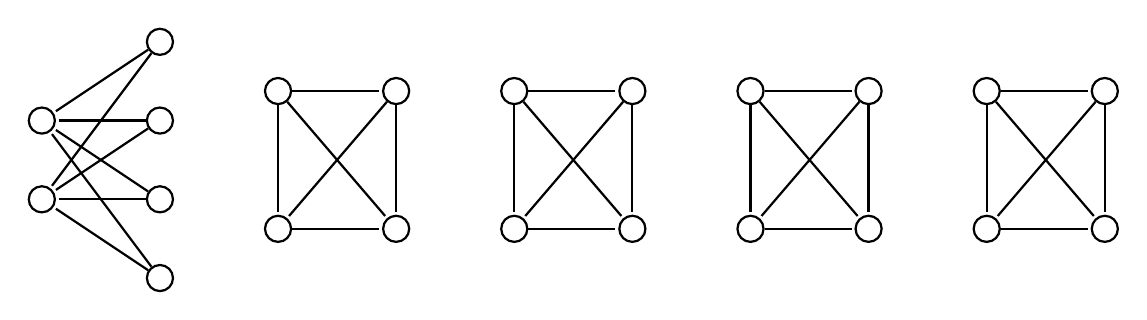
\begin{tikzpicture}[-,>=stealth,shorten >=1pt,auto,node distance=1.5cm, thick,main node/.style={scale=0.9,circle,draw,font=\sffamily\normalsize}]

                \node[circle, draw] (1) []{};
                \node[circle, draw] (2) [below of = 1, yshift = 0.5cm]{};
                \node[circle, draw] (3) [below of = 2, yshift = 0.5cm]{};
                \node[circle, draw] (4) [below of = 3, yshift = 0.5cm]{};
                \node[circle, draw] (5) [left of = 2]{};
                \node[circle, draw] (6) [left of = 3]{};

                \node[circle, draw] (7) [right of = 1, yshift = -0.625cm]{};
                \node[circle, draw] (8) [right of = 7]{};
                \node[circle, draw] (9) [right of = 4, yshift = 0.625cm]{};
                \node[circle, draw] (10) [right of = 9]{};

                \node[circle, draw] (11) [right of = 8]{};
                \node[circle, draw] (12) [right of = 11]{};
                \node[circle, draw] (13) [right of = 10]{};
                \node[circle, draw] (14) [right of = 13]{};

                \node[circle, draw] (15) [right of = 12]{};
                \node[circle, draw] (16) [right of = 15]{};
                \node[circle, draw] (17) [right of = 14]{};
                \node[circle, draw] (18) [right of = 17]{};

                \node[circle, draw] (19) [right of = 16]{};
                \node[circle, draw] (20) [right of = 19]{};
                \node[circle, draw] (21) [right of = 18]{};
                \node[circle, draw] (22) [right of = 21]{};

                % \path[every node/.style={font=\sffamily\small}]

                \draw[-] (1) to (5);
                \draw[-] (1) to (6);
                \draw[-] (2) to (5);
                \draw[-] (2) to (6);
                \draw[-] (3) to (5);
                \draw[-] (3) to (6);
                \draw[-] (4) to (5);
                \draw[-] (4) to (6);

                \draw[-] (7) to (8);
                \draw[-] (7) to (9);
                \draw[-] (7) to (10);
                \draw[-] (8) to (9);
                \draw[-] (8) to (10);
                \draw[-] (9) to (10);

                \draw[-] (11) to (12);
                \draw[-] (11) to (13);
                \draw[-] (11) to (14);
                \draw[-] (12) to (13);
                \draw[-] (12) to (14);
                \draw[-] (13) to (14);

                \draw[-] (15) to (16);
                \draw[-] (15) to (17);
                \draw[-] (15) to (18);
                \draw[-] (16) to (17);
                \draw[-] (16) to (18);
                \draw[-] (17) to (18);

                \draw[-] (19) to (20);
                \draw[-] (19) to (21);
                \draw[-] (19) to (22);
                \draw[-] (20) to (21);
                \draw[-] (20) to (22);
                \draw[-] (21) to (22);

                ;
            \end{tikzpicture}
            \caption{An example of the graph $G_2$, consisting of a $K_{2,4}$ and four $K_4$'s.}
        \end{figure}

        % We observe that $$\lim_{t \to + \infty}{\rho(K_{t, 2^t})} = \lim_{t \to \infty}{\dfrac{t \cdot 2^t}{t + 2^t}} = \lim_{t \to + \infty}{t}$$

        How does the algorithm compute when fed with $G_t$ as input? Since the degree of all the vertices of the cliques is exactly $t + 1$, and the complete bipartite graph $K_{t, 2^t}$ has vertices having degree $t$ --- namely, in its biggest partition --- the algorithm will compute as follows:

        \begin{itemize}
            \item initially, the algorithm will remove all the vertices of the biggest partition of $K_{t, 2^t}$ one by one, since they all have degree $t$, until only the $K_{t + 2}$-cliques remain
            \item then, the algorithm will proceed to remove all the vertices of the cliques, removing one $K_{t + 2}$-clique at a time, until no vertices remain
        \end{itemize}

        This implies that the possible graphs that the algorithm sees are the following:

        \begin{itemize}
            \item $G_t$, i.e. the graph in input
            \item for each iteration $i$ let $X_i$ be the set of vertices of the biggest partition of the complete bipartite graph that have been removed; then, we have the graph $G_t - X_i$, i.e. the remaining complete bipartite graph along with the $2^t$ $K_{t + 2}$-cliques
            % \item $(G_t - K_{t, 2^t}) \cup K_{t,t}$, i.e. the algorithm reached the point in which the two partitions of the complete bipartite graph have the same size --- we observe that from now on, the algorithm will always see a $K_{s, s}$ or a $K_{s, s-1}$ with $s < t$, which does not increase the density of the total graph, so we may ignore all of these cases
            \item $G - K_{t, 2^t}$, i.e. the $2^t$ $K_{t + 2}$-cliques --- we observe that from now on, the algorithm will always see a $K_s$ along with some amount of $K_{t + 2}$-cliques with $s \le t + 2$, which does not increase the density of the total graph, so we may ignore all of these cases
        \end{itemize}

        This concludes that we need to check the following densities in order to establish which result the algorithm returns:

        \begin{itemize}
            \item $\rho(G_t)=\dfrac{t \cdot 2^t + 2^t \cdot \binom{t + 2}{2}}{t + 2^t + 2^t \cdot (t + 2)} \stackrel{+ \infty}{\longrightarrow} \dfrac{t}{2}$
            \item $\rho(G_t - X_i) = \dfrac{t \cdot 2^t + 2 ^ t \cdot \binom{t+ 2}{2} - t \cdot i}{ t + 2^t + 2^t \cdot (t + 2) - i} \stackrel{+ \infty}{\longrightarrow} \dfrac{t}{2}$ --- we observe that this can be proven through the \href{https://en.wikipedia.org/wiki/Squeeze_theorem}{Squeeze theorem}, in fact \centeredeq{0.9}{$\displaystyle \dfrac{t}{2} = \lim_{t \to + \infty}{\dfrac{2^{t - 1}(t + 2)(t + 1)}{2^t(t + 3)}} = \lim_{t \to +\infty}{\rho(G_t - X_{2^t})} \le \lim_{t \to +\infty}{\rho(G - X_i)} \le \lim_{t \to + \infty}{\rho(G_t)} = \dfrac{t}{2}$}
            % \item $\rho((G_t - K_{t, 2^t}) \cup K_{t,t}) = \dfrac{t \cdot t + 2^t \cdot \binom{t + 2}{2}}{t + t + 2^t \cdot (t + 2)} \stackrel{+ \infty}{\longrightarrow} \dfrac{t}{2}$
            \item $\rho(G_t - K_{t, 2^t}) = \dfrac{2^t \cdot \binom{t + 2}{2}}{2^t \cdot (t + 2)} = \dfrac{t + 1}{2} \stackrel{+ \infty}{\longrightarrow} \dfrac{t}{2}$
        \end{itemize}

        This implies that for any set $S = \textsc{Charikar}(G_t)$ that the algorithm may yield, it holds that $$\lim_{t \to + \infty}{\rho(G_t[S])} = \dfrac{t}{2}$$

        However, it turns out that the densest subgraph of $G_t$ is actually $K_{t, 2^t}$, in fact $$\rho(K_{t, 2^t}) = \dfrac{t \cdot 2^t}{t + 2^t} \stackrel{+\infty}{\longrightarrow} t$$ and the algorithm \tit{never encounters $K_{t, 2^t}$}. Hence, we have that $$\lim_{t \to + \infty}{\dfrac{\rho(G_t[S])}{\rho(K_{t, 2^t})}} = \dfrac{\tfrac{t}{2}}{t} = \dfrac{1}{2}$$ or, in other words, it holds that $$\forall \varepsilon > 0 \quad \exists t \in \N \quad \rho(G_t[S]) < (\tfrac{1}{2} + \varepsilon) \rho(K_{t, 2^t}) \implies \mathrm{ALG_{DS}}(G_t) < (\tfrac{1}{2} + \varepsilon) \cdot \mathrm{OPT_{DS}}(G_t)$$
    }

    \begin{framedprob}{}
        Let $d$ be a cut metric. Prove that $d$ satisfies the triangle inequality.
    \end{framedprob}

    \solution{
        Let $d$ be defined over $T_1, \ldots, T_k$ and $\lambda_1, \ldots, \lambda_k >0$, i.e. $$d(x, y) := \sum_{i \in [k]}{\lambda_id_{T_i}(x, y)}$$ Fix $x$, $y$ and $z$; we observe that $$d(x, y) + d(y, z) = \sum_{i \in [k]}{\lambda_id_{T_i}(x, y)} + \sum_{i \in [k]}{\lambda_id_{T_i}(y, z)} = \sum_{i \in [k]}{\lambda_i \rbk {d_{T_i}(x, y) + d_{T_i}(y, z)}}$$ and since $d_{T_1}, \ldots, d_{T_k}$ are elementary cut metrics, they must satisfy the triangle inequality, therefore $$\sum_{i \in [k]}{\lambda_i \rbk {d_{T_i}(x, y) + d_{T_i}(y, z)}} \ge \sum_{i \in [k]}{\lambda_i d_{T_i}(x, z)} = d(x, z)$$ which proves that $d$ indeed satisfies the triangle inequality.
    }

    \begin{framedprob}{}
        Let $G = (V, E)$ be the graph with node set $V = [2n]$ for $n \in \N$, and edge set $$E = \{\{i, i + 1\} \mid 1 \le i \le 2n - 1\} \cup \{\{2n, 1\}\}$$ meaning that $G$ is a cycle on $2n$ nodes. Let $d_G$ be the shortest path metric on $G$. Prove that $d_G$ can be embedded isometrically into $\ell_1$.
    \end{framedprob}

    \solution{
        First, we observe that the shortest path metric on a $2n$-long cycle graph is defined as follows: $$\forall j, k \in [2n] \quad d_G(j, k) = \soe{ll}{\abs{k - j} & \abs{k - j} \le n \\ 2n - \abs{k - j} & \abs{k - j} > n}$$ Moreover, we observe that $\ell_1$ defined on two binary vectors $x, y \in \{0, 1\}^h$ is equivalent to their \href{https://en.wikipedia.org/wiki/Hamming_distance}{Hamming distance}, i.e. $$\ell_1(x, y) = d_H(x, y) = \abs{\{i : x_i \neq y_i\}}$$ and in particular $$\forall j, k \in [2n] \quad \ell_1(f(j), f(k)) = d_H(f(j), f(k))$$

        Now, consider the function $\func{f}{V(C_{2n})}{\R^n}$ defined as follows: $$\forall i \in [2n] \quad f(i) = \soe{ll}{0^{n - i + 1}1^{i - 1} & i \le n \\ 1^{2n - i + 1}0^{i - 1 - n} & i > n}$$ where the notation $0^a1^b$ stands for the vector $(\underbrace{0, \ldots, 0}_{a \ \mathrm{values}}, \underbrace{1, \ldots, 1}_{b \ \mathrm{values}}) \in \R^{a + b}$. At first, this definition of $f$ may seem counterintuitive, but if we consider each possible $f(i)$ the following nice pattern of \curlyquotes{sliding window} emerges:

    \begin{center}
        \begin{tabular}{c|c}
            \hline
            $i$ & $f(i)$ \\
            \hline\hline
            1 & 0000 \\
            \hline
            2 & 0001 \\ 
            \hline
            3 & 0011 \\
            \hline
            4 & 0111 \\
            \hline
            5 & 1111 \\
            \hline
            6 & 1110 \\
            \hline
            7 & 1100 \\
            \hline
            8 & 1000 \\
            \hline
        \end{tabular}
    \end{center}

        Finally, fix $j, k \in [2n]$, and without loss of generality suppose that $j < k$ -- in particular, this implies that $\abs{k - j} = k - j$. We have some cases to handle.

        \begin{itemize}
            \item $j, k \le n$; therefore, we have that
                \begin{itemize}
                    \item $j, k \le n \implies k - j \le n \implies d_G(j, k) = k - j$
                    \item $j < k \implies n - j + 1 > n - k + 1 \land j - 1 < k - 1$
                \end{itemize}
                and thus, to evaluate the Hamming distance between $f(j)$ and $f(k)$ we need to consider the \curlyquotes{middle} section in which the two binary vectors may differ
                \begin{equation*}
                    \begin{split}
                        \ell_1(f(j), f(k)) &= d_H(0^{n - j + 1}1^{j - 1}, 0^{n - k + 1}1^{k - 1}) \\
                                           &= [n - (j - 1)] - [(n - k + 1) + 1] + 1 \\
                                           &= [n - j + 1] - [n - k + 2] + 1 \\
                                           &= k - j \\
                                           &= d_G(j, k)
                    \end{split}
                \end{equation*}

            \item $j, k > n$; therefore, we have that
                \begin{itemize}
                    \item $j, k > n \implies k - j < n \implies d_G(j, k) = k - j$
                    \item $j < k \implies 2n - j + 1 > 2n - k + 1 \land j - 1 - n < k - 1 - n$
                \end{itemize}
                hence again, we just need to consider the \curlyquotes{middle} section in this case too
                \begin{equation*}
                    \begin{split}
                        \ell_1(f(j), f(k)) &= d_H(1^{2n - j + 1}0^{j - 1- n}, 1^{2n - k + 1}, 0^{k - 1- n}) \\
                                           &= [n - (k - 1- n)] - [(2n - j + 1) + 1] + 1 \\
                                           &= [n - k + 1 + n] - [2n - j + 2] + 1 \\
                                           &= k - j \\
                                           &= d_G(j, k)
                    \end{split}
                \end{equation*}

            \item $j \le n$ and $k < n$. We have two subcases
                \begin{enumerate}
                    \item $k - j \le n$; therefore, we have that
                        \begin{itemize}
                            \item $k - j \le n \implies d_G(j, k) = k - j$
                            \item $k - j \le n \implies n - j + 1 \le 2n - k + 1 \land j - 1 \ge k - n - 1$
                        \end{itemize}
                        and thus, in this case to evaluate the Hamming distance between $f(j)$ and $f(k)$ we need to consider the sections in which the two vectors can be 0 --- since they can only coincide when they are both 1
                        \begin{equation*}
                            \begin{split}
                                \ell_1(f(j), f(k)) &= d_H(0^{n - j + 1}1^{j - 1}, 1^{2n - k + 1}0^{k - 1- n}) \\
                                                   &= (n - j + 1) + (k - 1 - n) \\
                                                   &= k - j \\
                                                   &= d_G(j, k)
                            \end{split}
                        \end{equation*}
                    \item $k - j > n$; therefore, we have that
                        \begin{itemize}
                            \item $k - j > n \implies d_G(j, k) = 2n - k + j$
                            \item $k - j > n \implies n - j + 1 > 2n - k + 1 \land j - 1 < k - n - 1$
                        \end{itemize}
                        and thus, in this case to evaluate the Hamming distance between $f(j)$ and $f(k)$ instead we need to consider the sections in which the two vectors can be 1 --- since they can only coincide when they are both 0
                        \begin{equation*}
                            \begin{split}
                                \ell_1(f(j), f(k)) &= d_H(0^{n - j + 1}1^{j - 1}, 1^{2n - k + 1}0^{k - 1- n}) \\
                                                   &= (j - 1) + (2n - k + 1) \\
                                                   &= 2n - j + k \\
                                                   &= d_G(j, k)
                            \end{split}
                        \end{equation*}
                \end{enumerate}
        \end{itemize}
    }

    \begin{framedprob}[label={submod ex}]{}
        Prove that, for any $n \in \N$, if the function $\func{f}{\mathcal P([n])}{\R}$ has diminishing returns, it is submodular.
    \end{framedprob}

    \solution{
        First, we are going to prove a \tit{stronger} version of the diminishing return property, by extending it to \tit{subsets} of elements --- instead of single elements. The notation is a natural extension of the one we used so far.

        \claim{
            $\forall A \subseteq B \subseteq [n], C \subseteq [n] - B \quad \Delta_f(C \mid A) \ge \Delta_f(C \mid B)$.
        }{
            Fix three sets $A, B, C \subseteq [n]$ such that $A \subseteq B \subseteq [n]$ and $C \subseteq [n] - B$. Moreover, let $C := \{c_1, \ldots, c_k\}$, and for each $i \in [k]$ let $C_i := \{c_1, \ldots, c_i\}$. We proceed by induction on $i$.

            For the base case, we have that $C_1 = \{c_1\}$, hence by the diminishing return property we have that $$\Delta_f(C_1 \mid A) = \Delta_f(c_1 \mid A) \ge \Delta_f(c_1 \mid B) = \Delta_f(C_1 \mid B)$$ Now, assume inductively that the property holds for $C_{i - 1}$; then, we get that
            \begin{equation*}
                \begin{split}
                    \Delta_f(C_i \mid A) &= f(C_i \cup A) - f(A) \\
                                         &= f(\{c_1, \ldots, c_i\} \cup A) - f(A) \\
                                         &= f(\{c_1, \ldots, c_{i - 1}\} \cup \{c_i\} \cup A) - f(A) \\
                                         &= f(C_{i - 1} \cup \{c_i\} \cup A) - f(A) \\
                                         &= f(C_{i - 1} \cup \{c_i\} \cup A) - f(A) + f(C_{i - 1} \cup A) - f(C_{i - 1} \cup A) \\
                                         &= \Delta_f(C_{i - 1} \mid A) + \Delta_f(c_i \mid C_{i - 1} \cup A)
                \end{split}
            \end{equation*}
            Now, by applying induction on the first term, and the diminishing return property on the second term, we get that
            \begin{equation*}
                \begin{split}
                    \Delta_f(C_i \mid A) &= \Delta_f(C_{i - 1} \mid A) + \Delta_f(c_i \mid C_{i - 1} \cup A) \\
                                         &\ge \Delta_f(C_{i - 1} \mid B) + \Delta_f(c_i \mid C_{i - 1} \cup B) \\
                                         &= f(C_{i - 1} \cup B) - f(B) + f(\{c_i\} \cup C_{i - 1} \cup B) - f(C_{i - 1} \cup B) \\
                                         &= f(C_i \cup B) - f(B) \\
                                         &= \Delta_f(C_i \mid B)
                \end{split}
            \end{equation*}
        }

        Now, fix two sets $S, T \subseteq [n]$; note that it always holds that $(S \cap T) \subseteq T \subseteq [n]$ and $(S - T) \subseteq [n] - T$ for any choice of $S$ and $T$. Finally, through some algebraic manipulation, we get that
        \begin{equation*}
            \begin{split}
                     & \Delta_f(S - T \mid S \cap T) \ge \Delta_f(S - T \mid T) \\
                \iff & \Delta_f(S - (S \cap T) \mid S \cap T) \ge \Delta_f(S - ((S \cap T) \cup T) \mid (S \cap T) \cup T) \\
                \iff & f((S \cap T) \cup S) - f(S \cap T) \ge f((S \cap T) \cup S \cup T) - f((S \cap T) \cup T) \\
                \iff & f((S \cap T) \cup S) + f((S \cap T) \cup T) \ge f((S \cap T) \cup S \cup T) + f(S \cap T) \\
                \iff & f(S) + f(T) \ge f(S \cup T) + f(S \cap T)
            \end{split}
        \end{equation*}
        which proves that $f$ is indeed submodular.
    }

    \begin{framedprob}{}
        Given $n \in \N$, suppose that the function $\func{f}{\mathcal P([n])}{\R}$ satisfies the following property: $$\forall \{i, j\} \in \binom{[n]}{2}, S \subseteq [n] - \{i, j\} \quad f(S \cup \{i\}) + f(S \cup \{j\}) \ge f(S \cup \{i, j \}) + f(S)$$ Prove that $f$ has the diminishing returns property.
    \end{framedprob}

    \solution{
        Fix two sets $A \subseteq B \subseteq [n]$, and an element $x \in [n] - B$. Let $B - A = \{b_1, \ldots, b_m\}$ and for each $k \in [m]$ let $B_k := \{b_1, \ldots, b_k\}$. We claim the following.

        \claim{
            For any $k \in [m]$ it holds that $\Delta_f(x \mid A) \ge \Delta_f(x \mid A \cup B_k)$.
        }{
            We proceed by induction on $k$; consider $b_1 \in B - A$ --- and in particular $b_1 \neq x$; then clearly $A \subseteq [n] - \{x , b_1\}$ which means that we can use the property in the hypothesis as follows
            \begin{equation*}
                \begin{split}
                         & f(A \cup \{x\}) + f(A \cup \{b_1\}) \ge f(A \cup \{x, b_1\}) + f(A) \\
                    \iff & f(A \cup \{x\}) - f(A) \ge f(A \cup \{b_1\} \cup \{x\}) - f(A \cup \{b_1\}) \\
                    \iff & \Delta_f(x \mid A) \ge \Delta_f(x \mid A \cup \{b_1\}) = \Delta_f(x \mid A \cup B_1)
                \end{split}
            \end{equation*}
            Now, assume inductively that for $1 < k - 1 \le m$ it holds that $\Delta_f(x \mid A) \ge \Delta_f(x \mid B_{k - 1})$, and consider an element $b_k \in B - (A \cup B_{k - 1})$ --- and in particular $b_k \neq x$. Then, clearly $A \cup B_{k - 1} \subseteq [n] - \{x, b_k\}$ which means that we can use the property in the hypothesis as follows
            \begin{equation*}
                \begin{split}
                         & f(A \cup B_{k - 1} \cup \{x\}) + f(A \cup B_{k - 1} \cup \{b_k\}) \ge f(A \cup B_{k - 1} \cup \{x, b_k\}) + f(A \cup B_{k - 1}) \\
                    \iff & f(A \cup B_{k - 1} \cup \{x\}) + f(A \cup B_k) \ge f(A \cup B_k \cup \{x\}) + f(A \cup B_{k - 1}) \\
                    \iff & f(A \cup B_{k - 1} \cup \{x\}) - f(A \cup B_{k - 1}) \ge f(A \cup B_k \cup \{x\}) - f(A \cup B_k) \\
                    \iff & \Delta_f(x \mid A \cup B_{k - 1}) \ge \Delta_f(x \mid A \cup B_k)
                \end{split}
            \end{equation*}
            and by inductive hypothesis we get that $$\Delta_f(x \mid A) \ge \Delta_f(x \mid A \cup B_{k - 1}) \ge \Delta_f(x \mid A \cup B_k)$$
        }

        In particular, by the claim we have that for $k = m$ it holds that $$\Delta_f(x \mid A) \ge \Delta_f(x \mid A \cup B_m) = \Delta_f(x \mid A \cup B_{\abs{B - A}}) = \Delta_f(x \mid A \cup (B - A)) = \Delta_f(x \mid B)$$ which proves that $f$ has the diminishing returns property.
    }

    \begin{framedprob}{}
        Let $\func{f}{\powerset ([n])}{\R}$ be a modular function such that $f(\varnothing) = 0$.

        \begin{enumerate}
            \item Prove that the full description of $f$ (i.e. the value of $f(S)$ for any $S \subseteq [n]$) can be learned by querying the function $f$ on $O(n)$ sets.
            \item Let $G$ be a graph with $V(G) = [n]$ and $E(G) \subseteq \binom{V(G)}{2}$. Suppose that our algorithm is able to query $f$ only on the edges of $G$, i.e. we can query $f(\{i, j\})$ if and only if $\{i, j\} \in E(G)$. Can the algorithm learn the full description of $f$ if $G$ is a complete graph? What if $G$ is a tree? Give a general condition for the learnability of $f$.
        \end{enumerate}
    \end{framedprob}
    
    \solution{
        \hspace{0.7cm}

        \begin{enumerate}
            \item A function $\func{f}{\powerset([n])}{\R}$ is said to be \tit{learnable} if and only if for any input $S \subseteq [n]$ it holds that the value of $f(S)$ can be known. We claim the following.

                \claim{
                    A modular function $f$ is learnable if and only if $f(\varnothing), f(\{1\}), \ldots, f(\{n\})$ are known.
                }{
                    The direct implication trivially follows from the definition of learnability, so we only need to show the converse implication. We proceed by induction on the length of the input $\abs S = k$.

                    When $\abs S = 1$, we already know the values of $f(S)$ by hypothesis, so the base case trivially holds. Now, assume that the statement holds for $k - 1$ items, and consider a set $S$ of $k$ items. Then, by modularity of $f$, we know that $$f(S) = f(\{x_1, \ldots, x_k\}) = f(\{x_1, \ldots, x_{k - 1}\}) + f(\{x_k\})- f(\varnothing)$$ Hence, we observe that $f(\{x_1, \ldots, x_{k - 1}\})$ can be learned by inductive hypothesis, and since both $f(\{x_k\})$ and $f(\varnothing)$ are known by hypothesis, the claim holds.
                }
            \item We observe that in the previous exercise we did not use the fact that $f(\varnothing) = 0$, but we are going to leverage this property now. Consider a modular function $f$ that can be queried as described in the statement; through the claim of the previous exercise we proved that $f$ is learnable if and only if $f(\varnothing), f(\{1\}), \ldots, f(\{n\})$ are learnable. Thus, since $f(\varnothing)$ is given, we need to determine a general condition which allows us to find the values for $f(\{1\}), \ldots, f(\{n\})$ given only $f(\{i, j\})$ for each $\{i, j\} \in E(G)$.

                First, by modularity of $f$, we observe that $$\forall \{i, j\} \in E(G) \quad f(\{i,j \}) = f(\{i\}) + f(\{j\}) - f(\varnothing) = f(\{i\}) + f(\{j\})$$ since $f(\varnothing) = 0$. This condition is sufficient to construct a \tit{system of equations}. For instance, consider the graph $K_3$ with the vertices labeled $V(K_3) = \{1, 2, 3\}$: then, we construct the following: $$\soe{ll}{f(\{1\}) + f(\{2\}) = f(\{1, 2\}) \\ f(\{2\}) + f(\{3\}) = f(\{2, 3\}) \\ f(\{1\}) + f(\{3\}) = f(\{1, 3\})}$$ We observe that this system can be rewritten through matrices as follows $$\smat{1 & 1 & 0 \\ 0 & 1 & 1 \\ 1 & 0 & 1} \cdot \smat{f(\{1\}) \\ f(\{2\})  \\ f(\{3\})} = \smat{f(\{1, 2\}) \\ f(\{2, 3\}) \\ f(\{1, 3\})}$$ Can we solve this system? Through the \href{https://en.wikipedia.org/wiki/Gaussian_elimination}{Gaussian elimination} method we have that $$\smat{1 & 1 & 0 \\ 0 & 1 & 1 \\ 1 & 0 & 1} \longrightarrow \smat{1 & 1 & 0 \\ 0 & 1 & 1 \\ 0 & -1 & 1} \longrightarrow \smat{1 & 1 & 0 \\ 0 & 1 & 1 \\ 0 & 0 & 2}$$ which implies that the rank of the coefficient matrix is 3, and since we have 3 unknowns this system has unique solution.

                Can we generalize this concept? Fix an ordering $e_1, \ldots, e_m$ of $E(G)$, and an ordering $v_1, \ldots, v_n \in V(G)$, and for each subgraph $H \subseteq G$ let $A^H \in \R^{m \times n}$ be a coefficient matrix such that its $k$-th row is defined as follows $$A^H_k(i) = \soe{ll}{1 & i \in e_k \\ 0 & \mbox{otherwise}}$$ Similarly, let $b \in \R^m$ be a vector defined as $b = \sbk{f(e_1) \ \cdots \ f(e_{m_H})}^T$, and finally let $x = \sbk{x_1 \ \cdots \ x_{n_H}}^T$ for each $x_i = f(\{i\})$ --- where $m_H = \abs{E(H)}$ and $n_H = \abs{V(H)}$. It is clear that we can learn $f$ if and only if the system $A^Gx = b$ has a unique solution.

                \claim{
                    For each component $H_i$ of $G$, it holds that $A^{H_i}x = b$ has unique solution if and only if $H_i$ is not bipartite.
                }{
                    Let $n_{H_i} := \abs{V(H_i)}$; through linear algebra we know that $A^{H_i}x = b$ has unique solution if and only if the rank of the coefficient matrix is equal to the number of unknowns, which is $n_{H_i}$. Given a matrix $A$, the rank-nullity theorem states that $$\mathrm{rank}(A) + \dim(\ker \mathscr L_A) = n$$ where $\mathscr L_A$ is the function that describes the \tit{left application} of $A$, and $n$ is the number of \tit{columns} of $A$. Therefore, in our case it holds that $$\mathrm{rank}(A^{H_i}) + \dim(\ker \mathscr L_{A^{H_i}}) = n_{H_i}$$ Hence, to prove that $\mathrm{rank}(A^{H_i}) = n_{H_i}$ it suffices to show that $\dim(\ker \mathscr L_{A^{H_i}}) = 0$. This means that to prove our statement we have to show that the dimension of the kernel is 0 if and only if $H_i$ is not bipartite.

                    Assume that $H_i$ is not bipartite, and by way of contradiction suppose that there exists $\bar x = [f(v_1) \ \cdots \ f(v_{n_{H_i}})]^T \in \ker \mathscr L_{A^{H_i}}$ such that $\bar x \neq 0$. By definition, since $\bar x$ is in the kernel of $\mathscr L_{A^{H_i}}$, it holds that $A^{H_i} \bar x = 0$, and by construction of $A^{H_i}$ this happens if and only if for each edge $\{i, j\} \in E(H_i)$ it holds that $$f(\{i\}) + f(\{j\}) = 0 \iff f(\{i\}) = - f(\{j\})$$ This means that the values assigned to adjacent vertices \tit{are always the same but opposite in sign}: in other words, the vertices of $V(H_i)$ can be 2-colored such that

                    \begin{itemize}
                        \item one color class has color $a$
                        \item the other one has color $-a$
                    \end{itemize}

                    and since a graph is 2-colorable if and only if it is bipartite, this contradicts the assumption for which $H_i$ was not bipartite. This implies that all the $x \in \ker \mathscr L_{A^{H_i}}$ are such that $x = 0$, i.e. the kernel has dimension 0.

                    Vice versa, assume that $H_i$ is biparite through a bipartition $(A, B)$; consider the following function $\func{f}{\powerset([n])}{\R}$ such that $$\forall S \subseteq [n] \quad f(S) = \sum_{i \in S}{w(i)}$$ where $\func{w}{[n]}{\R}$ is a function defined as follows $$\forall i \in [n] \quad w(i) = \soe{ll}{1 & i \in A \\ -1 & i \in B}$$ which implies that $f(\varnothing) = 0$. Now, fix two sets $S, T \subseteq [n]$: we observe that $$S \cup T = (S - T) \cup (T - S) \cup (S \cap T)$$ which directly implies that
                    \begin{equation*}
                        \begin{split}
                            f(S) + f(T) &= \sum_{i \in S}{w(i)} + \sum_{i \in T}{w(i)} \\
                                        &= \rbk{ \sum_{i \in S - T}{w(v)} + \sum_{i \in S \cap T}{w(i)} } + \rbk{ \sum_{i \in T - S}{w(i)} + \sum_{i \in S \cap T}{w(i)} } \\
                                        % &= \sum_{i \in S - T}{w(i)} + \sum_{i \in T - S}{w(i)} + 2 \sum_{i \in S \cap T}{w(i)} \\
                                      % &= \rbk{ \sum_{i \in S - T}{w(i)} + \sum_{i \in T - S}{w(i)} + \sum_{i \in S \cap T} }
                                        &= \sum_{i \in S \cup T}{w (i)} + \sum_{i \in S \cap T}{w(i)} \\
                                        &= f(S \cup T) + f(S \cap T) \\
                        \end{split}
                    \end{equation*}
                    proving that $f$ is modular. This shows that $f$ is a possible input for our problem.

                    Fix an edge $\{i, j\} \in E(H_i)$, and without loss of generality suppose that $i \in A$ and $j \in B$; hence, by modularity of $f$ and by definition of $w$ it holds that $$f(\{i\}) + f(\{j\}) = w(i) + w(j) = 1 + (- 1) = 0$$ Since this is true for every edge, as previously observed this implies that $\bar x = [f(v_1) \ \cdots \ f(v_{n_{H_i}})]^T$ is inside the kernel of $\mathscr L_{A^{H_i}}$. Finally, by definition of $f$ it holds that $\bar x \neq 0$, meaning that the kernel contains non-zero vectors, i.e. $\mathscr L_{A^{H_i}} > 0$.
                }

                Let $S_G$ be the solution space of $A^Gx = b$. Similarly, for each $i \in [t]$ let $S_{H_i}$ be the solution space of $A^{H_i} x = b$. Clearly, it holds that $S_G = S_{H_1} \cap \ldots \cap S_{H_t}$. Hence, by the claim above we conclude that $S_G$ has a unique solution if and only if there is no bipartite component of $G$. Therefore, it holds that $f$ is learnable if and only if every component of $G$ has at least one odd-length cycle.

                In particular, this also concludes that $f$ can be learned when $G$ is a complete graph with at least 3 vertices, but not when $G$ is a tree.
        \end{enumerate}
    }

    \begin{framedprob}{}
        Consider the LP relaxation for Set Cover. Suppose that each element in the instance is part of at most $t$ sets. Give a rounding algorithm to the LP that returns a Set Cover solution whose cost is not larger than $t$ times the optimal cost.
    \end{framedprob}

    \solution{
        We observe that this exercise is very similar to the proof of \cref{lp 2-approx vc}.

        Consider an instance $(\mathcal U, C)$ of set cover such that each element $i \in \mathcal U$ is in at most $t$ sets. We observe the following.

        \claim{
            For any feasible solution $\{x_j\}_{j \in [m]}$ of the LP relaxation, and for any $i \in [n]$, if $i \in S_{j_1}, \ldots, S_{j_k}$ then there exists $j \in \{j_1, \ldots, j_k\}$ such that $x_j \ge \tfrac{1}{t}$.
        }{
            By way of contradiction, suppose that for any $j \in \{j_1, \ldots, j_k\}$ it holds that $x_j < \tfrac{1}{t}$. However, since $k \le t$ by the hypothesis on the instance of SC we chose, it holds that
            \begin{equation*}
                \begin{split}
                    \sum_{\substack{j \in[m] : \\ i \in S_j}}{x_j} &= \sum_{h = 1}^k{x_{j_h}} \\
                                                                   &= x_{j_1} + \ldots + x_{j_k} \\
                                                                   &< k \cdot \dfrac{1}{t} \\
                                                                   &\le t \cdot \dfrac{1}{t} \\
                                                                   &= 1
                \end{split}
            \end{equation*}
            implying that the solution $\{x_j\}_{j \in [m]}$ would violate the constraint of the LP, i.e. such solution would not be feasible $\lightning$.
        }

        Then, consider an optimal solution $\{\overline x_j\}_{j \in [m]}$ to the LP relaxation of SC over such instance, and consider the following set $$\abs{\overline S} = \cbk{S_j \in C \mid \overline x_j \ge \tfrac{1}{t}}$$ The previous claim immediately proves that $\overline S$ is a feasible solution to SC: in fact, by the claim it holds that for each element $i \in [n]$ there exists a set $S_j$ that contains $i$ such that $x_j \ge \tfrac{1}{t}$, i.e. $i$ will be covered by at least one set.

        Finally, to prove that this is a $t$-approximation of SC, consider an optimal solution $\{x^*_j\}_{j \in [m]}$ to the IP for SC, and construct $$S^* = \cbk{S_j \in C \mid x_j^* = 1}$$ Then, we get that
        \begin{equation*}
            \begin{alignedat}{2}
                \abs{\overline S} &= \sum_{S_j \in \overline S}{1} && \\
                                  &\le \sum_{S_j \in \overline S}{t \overline x_j} && \quad \quad (S_j \in \overline S \implies \overline x_j \ge \tfrac{1}{t} \iff t \overline x_j \ge 1) \\
                                  &= t \sum_{S_j \in \overline S}{ \overline x_j} && \\
                                  &\le t \sum_{S_j \in C}{\overline x_j} && \quad \quad (\overline S \subseteq C \land \overline x_j \ge 0) \\
                                  &\le t \sum_{S_j \in C}{x^*_j} \\
                                  &= t \abs{S^*}
            \end{alignedat}
        \end{equation*}
        where the last inequality comes from the fact that the constraints of the LP are \tit{weaker} than the ones of the IP.
    }

    \begin{framedprob}{}
        Consider the following algorithmic problem. A delivery company has access to a set $F$ of possible stocking facilities, and to a set of consumers $C$. Each consumer has to be served by one facility, and the company gains $G[c][f]$\euro \ if it serves consumer $c \in C$ with facility $f \in F$.

        If the company rents the set of facilities $S \subseteq F$, then the company will serve the generic client $c \in C$ with a facility $f \in S$ that maximizes $G[c][f]$. In particular, if the company rents the facilities of $S$, then its gain is $\sum_{c \in C}{\max_{f \in S}{G[c][f]}}$.

        Suppose that the company can rent at most $m$ facilites. Give an algorithm for approximately maximizing the gain of the company.
    \end{framedprob}

    \solution{
        We observe that this exercise is very similar to the proof of \cref{covering proof}.

        Let $g(S) = \sum_{c \in C}{\max_{f \in S}{G[c][f]}}$ be the gain of $S$, and for each customer $c \in C$ construct the following subfunction $$\forall c \in C \quad g_c(S) = \soe{ll}{\max_{f \in S}{G[c][f]} & S \neq \varnothing \\ 0 & \mbox{otherwise}}$$ This directly implies that $$g(S) = \sum_{c \in C}{g_c(S)}$$
        
        \claim{
            For all $c \in C$, the subfunction $g_c$ is non-negative, monotone increasing and submodular.
        }{
            First, fix a customer $c \in C$, and consider the subfunction $g_c$.

            Since the values inside the matrix $G$ are \euro's, $g_c$ is trivially non-negative.

            Now, fix two sets $S, T \subseteq F$ of facilities such that $S \subseteq T$: clearly, since $S$ is contained inside $T$, and $G$ is non-negative, it holds that $$\max_{f \in S}{G[c][f]} \le \max_{f \in T}{G[c][f]}$$ This proves that $g_c$ is monotone increasing.

            Lastly, fix two sets $S, T \subseteq F$ of facilities; to prove that $g_c$ is also submodular, we have three cases to handle.

            \begin{itemize}
                % \item If $S \cap T = \varnothing$, then clearly $$\max_{f \in S \cup T}{G[c][f]} = \max  \rbk{\{\max_{f \in S}{G[c][f]}, \max_{f \in T}{G[c][f]}\}}$$ therefore it holds that
                \item If $S \cap T = \varnothing$, let $M_S := g_c(S)$ and $M_T := g_c(T)$; we observe that clearly $g_c(S \cup T) = \max{\{M_S, M_T\}}$, therefore it holds that
                    \begin{equation*}
                        \begin{split}
                            g_c(S) + g_c(T) &= M_S + M_T \\
                                            &\ge \max\{M_S, M_T\} + 0 \\
                                            &= g_c(S \cup T) + f(\varnothing) \\
                                            &= g_c(S \cup T) + f(S \cap T)
                        \end{split}
                    \end{equation*}
                \item If $S \subseteq T$, let $M_S := g_c(S)$ and $M_T := g_c(T)$; we have two cases.

                    \begin{itemize}
                        \item If $M_S = M_T$, then $g_c(S \cup T) = M_S = M_T$, therefore
                            \begin{equation*}
                                \begin{split}
                                    g_c(S) + g_c(T) &= M_S + M_T \\
                                                    &= M_S + M_S \\
                                                    &= g_c(S \cup T) + g_c(S) \\
                                                    &= g_c(S \cup T) + g_c(S \cap T)
                                \end{split}
                            \end{equation*}
                        \item If $M_S \neq M_T$, then $M_T = g_c(M - T)$ --- otherwise $M_T$ would violate the maximality of $M_S$ --- which in turn implies that $M_T > M_S$ --- otherwise $M_S$ would have been a maximum for $T$ as well. Therefore, it holds that $g_c(S \cup T) = M_T = g_c(T)$, hence
                            \begin{equation*}
                                \begin{split}
                                    g_c(S) + g_c(T) &= M_S + M_T \\
                                                    &= g_c(S) + g_c(T) \\
                                                    &= g_c(S \cap T) + g_c(S \cup T)
                                \end{split}
                            \end{equation*}
                    \end{itemize}
                \item If $S - T, T - S \neq \varnothing$, let $M_S := g_c(S)$, $M_T := g_c(T)$ and $M_{S \cap T} = g_c(S \cap T)$; we have three cases.

                    \begin{itemize}
                        \item If $M_S = M_T = M_{S \cap T}$ then $g_c(S \cup T) = M_S = M_T = M_{S \cap T}$ therefore
                            \begin{equation*}
                                \begin{split}
                                    g_c(S) + g_c(T) &= M_S + M_T \\
                                                    &= M_{S \cap T} + M_{S \cap T} \\
                                                    &= g_c(S \cup T) + g_c(S \cap T)
                                \end{split}
                            \end{equation*}
                        \item If $M_S = M_{S \cap T} \neq M_T$ --- the case in which $M_T = M_{S \cap T} \neq M_S$ is analogous --- then $M_T > M_S$ otherwise $M_S$ would have been maximum for $T$ as well. Therefore, it holds that $g_c(S \cup T) = M_T = g_c(T)$, hence
                            \begin{equation*}
                                \begin{split}
                                    g_c(S) + g_c(T) &= M_S + M_T \\
                                                    &= M_{S \cap T} + g_c(S \cup T) \\
                                                    &= g_c(S \cap T) + g_c(S \cup T)
                                \end{split}
                            \end{equation*}
                        \item If $M_S$, $M_T$ and $M_{S \cap T}$ are all distinct, then $M_S, M_T > M_{S \cap T}$ otherwise $M_{S \cap T}$ would violate the maximality of $M_S$ and $M_T$ for $S$ and $T$ respectively. Therefore, it holds that $g_c(S \cup T) = \max\{M_S, M_T\} > M_{S \cap T}$, hence
                            \begin{equation*}
                                \begin{split}
                                    g_c(S) + g_c(T) &= M_S + M_T \\
                                                    &\ge \max \{M_S, M_T\} + M_{S \cap T} \\
                                                    &= g_c(S \cup T) + g_c(S \cap T)
                                \end{split}
                            \end{equation*}
                    \end{itemize}
            \end{itemize}
        }

        By the claim, it trivially follows that $g$ is both non-negative and monotone increasing. Finally, fix two sets $S, T \subseteq F$ of facilities; show that it is also submodular, we can leverage the submodularity of $g_c$ for each $c \in C$ as follows:
        \begin{equation*}
            \begin{split}
                g(S) + g(T) &= \sum_{c \in C}{g_c(S)} + \sum_{c \in C}{g_c(T)} \\
                            &= \sum_{c \in C}{\rbk{g_c(S) + g_c(T)}} \\
                            &\ge \sum_{c \in C}{\rbk{g_c(S \cup T) + g_c(S \cap T)}} \\
                            &= \sum_{c \in C}{g_c(S \cup T)} + \sum_{c \in C}{g_c(S \cap T)} \\
                            &= g(S \cup T) + g(S \cap T)
            \end{split}
        \end{equation*}

        Therefore, since the gain of $S$ is non-negative, monotone increasing and submodular, for any $m$ maximum number of facilities that the company can rent we can employ \cref{nwf approx} to return a set of $m$ facilities with an approximation ratio of $1 - \tfrac{1}{e}$ by \cref{nwf approx proof}.
    }

    \begin{framedalgo}{The $f$-Generalized W.M. Expert model}
        Given a set $M$ of $n$ trained experts, the algorithm yields predictions over time $T$. \\
        \hrule

        \quad
        \begin{algorithmic}[1]
            \Function{weightedMajorityExpertModel}{$M$, $T$, $f$}
                \For{$i \in [n]$}
                    \State $w_i := 0$
                \EndFor
                \For{$t \in [T]$}
                    \State Read $y_t = [y_{1, t} \ \cdots \ y_{n, t}]$
                    \State $A_t := \sum\limits_{\substack{i \in [n] : \\ y_{i , t} = 1}}{f(w_i)}$
                    \State $B_t := \sum\limits_{\substack{i \in [n] : \\ y_{i , t} = 0}}{f(w_i)}$
                    \If{$A_t \ge B_t$}
                        \State $z_t := 1$
                    \Else
                        \State $z_t := 0$
                    \EndIf
                    \State Read the outcome $x_t \in \{0, 1\}$
                    \If{$x_t \neq z_t$}
                        \For{$i \in [n]$}
                            \If{$y_{i, t} \neq x_t$}
                                % \State $w_i = \tfrac{w_i}{2}$
                                \State $w_i = w_i + 1$
                            \EndIf
                        \EndFor
                    \EndIf
                \EndFor
            \EndFunction
        \end{algorithmic}
    \end{framedalgo}

    \begin{framedprob}{}
        Consider the algorithm above: this is the $f$-Generalized Weighted Majority Expert model, which is a generalized version of \cref{wmem}. In fact, if $f(w_i) = 2^{-w_i}$ then the two algorithms are identical, and it guarantees a number of mistakes not larger than $O(m^* + \log n)$ where $m^*$ is the number of mistakes of the best expert, and $n$ is the number of experts --- as we proved in \cref{wmem proof}.

        Prove that, if $f(w_i) = \tfrac{w_i}{w_i + 1}$, then the number of mistakes of the $f$-Generalized Weighted Majority algorithm is $\Omega(n)$ even in cases where $m^* = 0$.

        Moreover, prove that if $f(w_i) = (w_i + 1)^{- \alpha}$ for a generic constant $\alpha > 0$, then there are instances with $m^* =0$ where the $f$-Generalized Weighted Majority algorithm makes a number of mistakes polynomial in $n$.
    \end{framedprob}

    \solution{
        The first approach that we may try is the one used in the proof of \cref{wmem proof} itself. In fact, in that version of the algorithm we were able to prove that $W^{(t + 1)} \le \tfrac{3}{4} W^{(t)}$, however the value $\tfrac{3}{4}$ directly derives from the \tit{updating rule} of the weights. In particular, since the weights of each wrong expert is \tit{halved}, it holds that $$W^{(t + 1)} = \dfrac{I^{(t)}}{2} + (W^{(t)} - I^{(t)})$$ since the \tit{total} weight of the wrong experts is halved as well, and the second term of the sum is the remaining total weight --- i.e. the sum of the weights of the experts who were \tit{right}.

        Can we employ a similar approach in this second setting? First, we need to understand how to get $w^{(t + 1)}_i$ given $w^{(t)}_i$ if the $i$-th expert was wrong --- which is not explicit in the $f$-Generalized version. We observe that $f (w_i^{(t)}) = \tfrac{1}{k}$ and $f (w_i^{(t + 1)}) = \tfrac{1}{k + 1}$ --- for $k \ge 1$, implying that $$k = \dfrac{1}{f (w_i^{(t)})} \implies f (w_i^{(t + 1)}) = \dfrac{1}{k + 1} = \dfrac{1}{\tfrac{1}{f (w_i^{(t)})} + 1} = \dfrac{f (w_i^{(t))}}{1 + f (w_i^{(t)})}$$ which means that we can rewrite the $f$-Generalized version by setting all the weights $w_i^{(0)} := 1$ at the beginning, and then use the following \tit{updating rule} $$w_i := \dfrac{w_i}{1 + w_i}$$ From now on, we will use this version of the $f$-Generalized variant of the algorithm, in order to reason more clearly w.r.t. the updating rule we are using.

        In particular, this updating rule implies that the equation for $W^{(t + 1)}$ does not hold anymore, for two reasons:

        \begin{itemize}
            \item we are not \tit{halving} the wrong weights anymore, but we are decreasing $I^{(t)}$ by an amount that directly depends on the weights themselves
            \item even assuming that $$W^{(t + 1)} = \varepsilon I^{(t)} + (W^{(t)} - I^{(t)})$$ for some amount $\varepsilon > 0$ would not be correct, because the amount directly depends on the weights, therefore $\varepsilon$ \tit{changes over time} and cannot be assumed to be a constant value
        \end{itemize}

        In conclusion, this suggests that a different approach is needed in order to prove that $m = \Omega(n)$, even for $m^* = 0$.

        In fact, an \tit{adversarial argument} suffices to prove such lower bound on $m$, and the answer lies in how the updating rule operates. In particular, starting from $w_i = 1$, we get that each time the $i$-th expert is wrong $w_i$ is transformed as follows: $$1 \stackrel{f}{\longrightarrow} \dfrac{1}{2} \stackrel{f}{\longrightarrow} \dfrac{1}{3} \stackrel{f}{\longrightarrow} \ldots$$ which is precisely the harmonic sequence. In other words, after $k$ mistakes of the $i$-th expert, it holds that $w_i = h_k = \tfrac{1}{k}$, where $h_k$ is the $k$-th member of the harmonic sequence.

        Hence, consider a set of $n$ experts such that $m^* = 0$ --- i.e. the best expert makes no mistakes, which means that there is at least one perfect expert. Let the first expert be the perfect one, and all the other $n - 1$ experts be such that they always answer 0. Then, suppose that the correct answer is \tit{always 1}. Thus, we have that

        \begin{itemize}
            \item the perfect expert is always correct, hence $w_1^{(t)} = 1$ for any $t \in [0, T]$
            \item all the other experts are wrong \tit{at each iteration}, hence $w_i^{(t)} = \tfrac{1}{t + 1}$ for each $i = [2, n]$ and for each $t \in [0, T]$
        \end{itemize}

        implying that when $t < n - 2$ it holds that $$A_t = \sum_{\substack{i \in [n] : \\ y_{i, t} = 1}}{w_i^{(t)}} = 1 = (n - 1) \cdot \dfrac{1}{n - 1} < (n - 1) \cdot \dfrac{1}{t + 1} = \sum_{\substack{i \in [n] : \\ y_{i, t} = 0}}{w_i^{(t)}} = B_t$$ which means that for the first $n - 2$ iterations (we start at $t = 0$) the algorithm is \tit{forced to be wrong}. This implies that $m \ge n - 2$, and by choosing for instance $c = \tfrac{1}{2}$ and $n_0 = 4$ we get that $$\forall n \ge n_0 \quad m \ge c \cdot n \implies m = \Omega(n)$$

        Lastly, if we assume that $f(w_i) = (w_i + 1)^{-\alpha}$ for some $\alpha > 0$ we observe that the weights now change as follows $$1 \stackrel{f}{\longrightarrow} \dfrac{1}{2^\alpha} \stackrel{f}{\longrightarrow} \dfrac{1}{3^\alpha} \stackrel{f}{\longrightarrow} \ldots$$ which implies that $w_i = \rbk{h_k}^\alpha = \tfrac{1}{k^\alpha}$. Therefore, we can employ the same adversary argument to find a lower bound on $m$, but this time to determine the number of iterations in which our algorithm is forced to be wrong we need $t$ to be such that $$1 < \dfrac{n - 1}{(1 + t)^\alpha} \iff (1 + t)^\alpha < n - 1 \implies t < (n - 1)^{\tfrac{1}{\alpha}} - 1$$ and since we start at $t = 0$, this implies that $$m \ge (n - 1)^{\tfrac{1}{\alpha}} - 1 \implies m = \Omega \rbk{n^{1/\alpha}}$$
    }

    \printbibliography % UNCOMMENT FOR BIBLIOGRAPHY

\end{document}
